% Author: Alfredo Sánchez Alberca (asalber@ceu.es)
% !TEX program = xelatex
%----------------------------------------------------------------------------------------
%    DOCUMENT CLASS
%----------------------------------------------------------------------------------------

\documentclass[11pt,a4paper,openright]{book}
  %----------------------------------------------------------------------------------------
  %	PACKAGES AND OTHER DOCUMENT CONFIGURATIONS
  %----------------------------------------------------------------------------------------
  
  % Language settings
  \usepackage{polyglossia}
  \setdefaultlanguage{spanish}
  
  % Margins and layout
  \usepackage[top=3cm, bottom=3cm, left=2.54cm, right=2.54cm]{geometry}
  
  % Math support
\usepackage{amsmath, amssymb}
 % \usepackage{mathspec}

  % Font settings
  \usepackage{unicode-math}
  \setmainfont[Ligatures=TeX]{TeX Gyre Pagella}
  \setmathfont{TG Pagella Math}
  % \setmathfont[math-style=ISO, bold-style=ISO]{texgyrepagella-math.otf}
  
  % Color
  \usepackage{xcolor} % Required for specifying colors by name
  \definecolor{color1}{RGB}{5,161,230}
  \definecolor{color2}{RGB}{238,50,36}
  \definecolor{ocre}{RGB}{243,102,25} % Define the orange color used for highlighting throughout the book
  \definecolor{blueceu}{RGB}{5,161,230} % Blue color of CEU logo
  \definecolor{greenceu}{RGB}{185,209,16} % Green color of CEU logo
  \definecolor{redceu}{RGB}{238,50,36} % Red color of CEU logo
  \definecolor{grayceu}{RGB}{111,107,83} % Gray color of CEU logo
  \definecolor{coral}{rgb}{1,0.5,0.31} % Orange color for graphics
  \definecolor{royalblue1}{rgb}{0.28,0.46,1} % Blue color for graphics
  \definecolor{mygreen}{rgb}{0,0.8,0} % Green color for graphics
  \definecolor{chaptergrey}{RGB}{5,161,230} % Blue color of CEU logo

  % Line breaking
  \usepackage{microtype} 
  \setlength{\emergencystretch}{2em}
  
  % Graphics
  \usepackage{graphicx}
  \usepackage{tikz} 
  \usepackage{eso-pic} % Required for specifying an image background in the title page
  
  % Arrays and tables
  \usepackage{array}
  \usepackage{multirow}
  \usepackage{colortbl}
  \usepackage{booktabs}
  \newcommand{\tcrule}{\arrayrulecolor{color1!50!white}\toprule}
  \newcommand{\mcrule}{\arrayrulecolor{color1!50!white}\midrule}
  \newcommand{\bcrule}{\arrayrulecolor{color1!50!white}\bottomrule}
  
  % Captions
  \usepackage[margin=20pt, font=small, labelfont=bf, labelsep=endash]{caption}
  
  % Floating figures
  \usepackage{subfigure}
  
  % Lists
  \usepackage[shortlabels]{enumitem} % Customize lists
  %\setlist{nolistsep} % Reduce spacing between bullet points and numbered lists
  \setlist[description]{style=sameline,leftmargin=0cm}

  % Columns
  \usepackage{multicol}
  
  % \makeatletter
  % \let\savees@listquot\es@listquot
  % \def\es@listquot{\protect\savees@listquot}
  % \makeatletter

  % hyperlinks
  \usepackage{hyperref}
  \hypersetup{
  pdfauthor = {Alfredo S\'anchez Alberca},
  pdftitle = {Prácticas de Cálculo con Geogebra},
  pdfsubject = {Cálculo},
  pdfkeywords = {Matemáticas, Cálculo, Geogebra},
  pdfcreator = {XeLaTeX with hyperref package},
  pdfproducer = {pdfLaTeX},
  colorlinks = true,
  linkcolor = red,          % color of internal links
  citecolor = green,        % color of links to bibliography
  filecolor = magenta,      % color of file links
  urlcolor = magenta,          % color of external links
  }
  %\usepackage{breakurl}
  
  % Indentation
  %\setlength\parindent{0pt}
  
  % Control of widow orphan lines
  \clubpenalty=10000
  \widowpenalty=10000 
  
  %Code listing formatting
  \usepackage{listings}
  \lstdefinelanguage{morejava}{morekeywords={String}}
  \definecolor{vollgrau}{rgb}{0.9,0.9,0.9}
  \definecolor{colKeys}{rgb}{0,0,1}
  \definecolor{colIdentifier}{rgb}{0,0,0}
  \definecolor{colComments}{rgb}{1,0.5,0}
  \definecolor{colString}{rgb}{0,0.5,0}
  \definecolor{colbackground}{rgb}{0.9,0.9,1}
  \lstset{%
       language=R,
       float=hbp,%
       basicstyle=\ttfamily,%
       identifierstyle=\color{colIdentifier},%
       keywordstyle=\color{colKeys},%
       stringstyle=\color{colString},%
       commentstyle=\color{colCommentsxelatex},%
  %    columns=flexible,%xelatex
  %    columns=fullflexible,%xelatex
       columns=fixed, %xelatex
       tabsize=1,%xelatex
       extendedchars=true,%xelatex
       showspaces=false,%xelatex
       showstringspaces=false,%xelatex
       breaklines=true,%xelatex
       breakindent=10pt,%xelatex
       backgroundcolor=\color{colbackgxelatexround},%
       breakautoindent=true,%xelatex
       captionpos=t,%
       xleftmargin=1em,%
  %    xrightmargin=.5\fboxsep,%
       numbersep=1em,%
       escapechar=\#\RequirePackage[\eu@zf@math]{fontspec}[2008/08/09]
  }
  
  % Set short or lon\RequirePackage[\eu@zf@math]{fontspec}[2008/08/09]ersion desired
  % \usepackage[cort\RequirePackage[\eu@zf@math]{fontspec}[2008/08/09]
  
  %----------------------------------------------------------------------------------------
%	SECTIONS AND SUBSECTIONS
%----------------------------------------------------------------------------------------
%\titleformat*{\section}{\Huge}
%\titleformat*{\subsection}{\Large}


% Chapter and section formatting 
\usepackage[rigidchapters,explicit]{titlesec}
\setlength{\fboxsep}{5pt}
\newlength{\titulolength}
\setlength{\titulolength}{\textwidth} 
\addtolength{\titulolength}{-2\fboxsep}
\addtolength{\titulolength}{-2\fboxrule}
\titleformat{\chapter}[display]
{\bfseries\sffamily}
{\filleft \mdseries \LARGE \color{blueceu} Práctica \Huge\thechapter}
{0.5ex}
{\colorbox{blueceu}{\parbox[t]{\titulolength}{\rule{0mm}{10mm}\Huge\sffamily\filleft\textcolor{white}{#1}}}}
\titleformat{\section}{\normalfont\Large\bfseries\color{blueceu}}{\arabic{section}}{1em}{#1}
\titleformat{\subsection}{\normalfont\large\bfseries\color{blueceu}}{\arabic{section}.\arabic{subsection}}{1em}{#1}
\titleformat{\subsubsection}{\normalfont\normalsize\bfseries\color{blueceu}}{\arabic{section}.\arabic{subsection}.\arabic{subsubsection}}{0.5em}{#1}
\titlespacing{\chapter}{0pt}{0pt}{30ex}
\titlespacing{\section}{0pt}{8ex}{4ex}

%----------------------------------------------------------------------------------------
%	MAIN TABLE OF CONTENTS
%----------------------------------------------------------------------------------------

% \usepackage{titletoc} % Required for manipulating the table of contents
% 
% \contentsmargin{0cm} % Removes the default margin
% % Chapter text styling
% \titlecontents{chapter}[1.25cm] % Indentation
% {\addvspace{15pt}\large\bfseries} % Spacing and font options for chapters
% {\color{gray}\contentslabel[\Large\thecontentslabel.]{1.25cm}} % Chapter number
% {}  
% {\color{gray}\bfseries\hfill\thecontentspage} % Page number
% % Section text styling
% \titlecontents{section}[1.25cm] % Indentation
% {\addvspace{5pt}\bfseries} % Spacing and font options for sections
% {\contentslabel[\thecontentslabel]{1.25cm}} % Section number
% {}
% {\hfill\color{black}\thecontentspage} % Page number
% []
% % Subsection text styling
% \titlecontents{subsection}[1.25cm] % Indentation
% {\addvspace{1pt}\small} % Spacing and font options for subsections
% {\contentslabel[\thecontentslabel]{1.25cm}} % Subsection number
% {}
% {\;\titlerule*[.5pc]{.}\;\thecontentspage} % Page number
% [] 

%----------------------------------------------------------------------------------------
%	MINI TABLE OF CONTENTS IN CHAPTER HEADS
%----------------------------------------------------------------------------------------

% % Section text styling
% \titlecontents{lsection}[0em] % Indendating
% {\footnotesize\sffamily} % Font settings
% {}
% {}
% {}
% 
% % Subsection text styling
% \titlecontents{lsubsection}[.5em] % Indentation
% {\normalfont\footnotesize\sffamily} % Font settings
% {}
% {}
% {}
 
%----------------------------------------------------------------------------------------
%	PAGE HEADERS
%----------------------------------------------------------------------------------------

% Headings and footers
\usepackage{fancyhdr}
\pagestyle{fancy}
\fancyhead{}
\renewcommand{\chaptermark}[1]{\markboth{\thechapter.\ #1}{}}
\fancyhead[LE]{\scshape Matemática Aplicada con Geogebra}
\fancyhead[RO]{\sffamily\slshape \leftmark}
\renewcommand{\headrulewidth}{0pt}
\renewcommand{\floatpagefraction}{.8}
\renewcommand{\textfraction}{.1}


% \usepackage{fancyhdr} % Required for header and footer configuration
% 
% \pagestyle{fancy}
% \renewcommand{\chaptermark}[1]{\markboth{\color{grayceu}\sffamily\normalsize\textit{#1}}{}} % Chapter text font
% % settings
% %\renewcommand{\sectionmark}[1]{\markright{\color{grayceu}\sffamily\normalsize\textit{\thesection\hspace{5pt}#1}}{}} %
% % Section text font settings
% \fancyhf{} \fancyfoot[LE,RO]{\normalsize\thepage} % Font setting for the page number in the footer
% \fancyhead[RE]{{\color{grayceu}\sffamily\normalsize\textit{Pr�cticas de Bioestad�stica con R and RKTeaching}}} % Print the nearest
% % section name on the left side of odd pages
% \fancyhead[LO]{\leftmark} % Print the current chapter name on the right side of even pages
% \renewcommand{\headrulewidth}{0pt} % Removes the rule in the header
% \addtolength{\headheight}{2.5pt} % Increase the spacing around the header slightly
% \renewcommand{\footrulewidth}{0pt} % Removes the rule in the footer
% \fancypagestyle{plain}{\fancyhead{}\renewcommand{\headrulewidth}{0pt}} % Style for when a plain pagestyle is specified
% 
% % Removes the header from odd empty pages at the end of chapters
% \makeatletter
% \renewcommand{\cleardoublepage}{
% \clearpage\ifodd\c@page\else
% \hbox{}
% \vspace*{\fill}
% \thispagestyle{empty}
% \newpage
% \fi}


%----------------------------------------------------------------------------------------
%	THEOREM STYLES
%----------------------------------------------------------------------------------------

\usepackage{amsthm} % For including math equations, theorems, symbols, etc

\newcommand{\intoo}[2]{\mathopen{]}#1\,;#2\mathclose{[}}
\newcommand{\ud}{\mathop{\mathrm{{}d}}\mathopen{}}
\newcommand{\intff}[2]{\mathopen{[}#1\,;#2\mathclose{]}}
\newtheorem{notation}{Notación}[chapter]

\newtheoremstyle{blueceu} % Theorem style name
{7pt} % Space above
{7pt} % Space below
{\normalfont} % Body font
{} % Indent amount
{\small\bf\sffamily\color{blueceu}} % Theorem head font
{\;\;} % Punctuation after theorem head
{0.25em} % Space after theorem head
{\small\sffamily\color{blueceu}\thmname{#1}\thmnumber{\@ifnotempty{#1}{ }\@upn{#2}} % Theorem text (e.g. Theorem 2.1)
\thmnote{\ {\the\thm@notefont\sffamily\bfseries\color{blueceu}--- #3.}}} % Optional theorem note
\renewcommand{\qedsymbol}{$\blacksquare$} % Optional qed square

\newtheoremstyle{blacknumex} % Theorem style name
{7pt} % Space above
{7pt} % Space below
{\normalfont} % Body font
{} % Indent amount
{\small\bf\sffamily} % Theorem head font
{\;\;} % Punctuation after theorem head
{0.25em} % Space after theorem head
{\small\sffamily{\tiny\ensuremath{\blacksquare}}\ \thmname{#1}\thmnumber{\@ifnotempty{#1}{ }\@upn{#2}} % Theorem text (e.g. Theorem 2.1)
\thmnote{\ {\the\thm@notefont\sffamily\bfseries--- #3.}}} % Optional theorem note

\newtheoremstyle{blacknum} % Theorem style name
{7pt} % Space above
{7pt} % Space below
{\normalfont} % Body font
{} % Indent amount
{\small\bf\sffamily} % Theorem head font
{\;\;} % Punctuation after theorem head
{0.25em} % Space after theorem head
{\small\sffamily\thmname{#1}\thmnumber{\@ifnotempty{#1}{ }\@upn{#2}} % Theorem text (e.g. Theorem 2.1)
\thmnote{\ {\the\thm@notefont\sffamily\bfseries--- #3.}}} % Optional theorem note

\newtheoremstyle{example} % Theorem style name
{7pt} % Space above
{7pt} % Space below
{\normalfont} % Body font
{} % Indent amount
{\small\bf\sffamily} % Theorem head font
{\;\;} % Punctuation after theorem head
{0.25em} % Space after theorem head
{\small\sffamily\thmname{#1} % Theorem text (e.g. Theorem 2.1)
\thmnote{\ {\the\thm@notefont\sffamily\bfseries--- #3.}}} % Optional theorem note

\newtheoremstyle{indication} % Theorem style name
{-5pt} % Space above
{7pt} % Space below
{\normalfont} % Body font
{-28pt} % Indent amount
{\bf} % Theorem head font
{\kern-11.5pt} % Punctuation after theorem head
{20pt} % Space after theorem head
{\begin{tikzpicture}
\draw node [fill=blueceu,opacity=1,inner sep=1pt] {\makebox[17pt][c]{\includegraphics[scale=0.3]{img/bulb}}}; \end{tikzpicture}} % Theorem text (e.g. Theorem 2.1)

\makeatother

% Defines the theorem text style for each type of theorem to one of the three styles above
\theoremstyle{ocrenum}
\newtheorem{exerciseT}{Exercise}[chapter]
\theoremstyle{blacknumex}
\newtheorem{exampleT}{Example}[chapter]
%\theoremstyle{blacknum}
\theoremstyle{blueceu}
\newtheorem{vocabulary}{Vocabulario}[chapter]
\newtheorem{definitionT}{Definición}[chapter]
\newtheorem{theoremT}{Teorema}[chapter]
\newtheorem{corolary}{Corolario}[chapter]
\theoremstyle{indication}
\newtheorem{indicationT}{Indicación}
%\theoremstyle{example}
%\newtheorem{ejemplo}{Ejemplo}

%----------------------------------------------------------------------------------------
%	DEFINITION OF COLORED BOXES
%----------------------------------------------------------------------------------------

\RequirePackage[framemethod=default]{mdframed} % Required for creating the theorem, definition, exercise and corollary boxes

% Theorem box
\newmdenv[skipabove=7pt,
skipbelow=7pt,
backgroundcolor=black!5,
linecolor=ocre,
innerleftmargin=5pt,
innerrightmargin=5pt,
innertopmargin=5pt,
leftmargin=0cm,
rightmargin=0cm,
innerbottommargin=5pt]{tBox}

% Exercise box	  
\newmdenv[skipabove=7pt,
skipbelow=7pt,
rightline=false,
leftline=true,
topline=false,
bottomline=false,
backgroundcolor=ocre!10,
linecolor=ocre,
innerleftmargin=5pt,
innerrightmargin=5pt,
innertopmargin=5pt,
innerbottommargin=5pt,
leftmargin=0cm,
rightmargin=0cm,
linewidth=4pt]{eBox}	

% Definition box
\newmdenv[skipabove=10pt,
skipbelow=10pt,
rightline=false,
leftline=true,
topline=false,
bottomline=false,
linecolor=ocre,
innerleftmargin=5pt,
innerrightmargin=5pt,
innertopmargin=0pt,
leftmargin=0cm,
rightmargin=0cm,
linewidth=4pt,
innerbottommargin=0pt]{dBox}	

% Corollary box
\newmdenv[skipabove=7pt,
skipbelow=7pt,
rightline=false,
leftline=true,
topline=false,
bottomline=false,
linecolor=gray,
backgroundcolor=black!5,
innerleftmargin=5pt,
innerrightmargin=5pt,
innertopmargin=5pt,
leftmargin=0cm,
rightmargin=0cm,
linewidth=4pt,
innerbottommargin=5pt]{cBox}	

% Indication box
\newmdenv[skipabove=7pt,
skipbelow=7pt,
rightline=false,
leftline=true,
topline=false,
bottomline=false,
linecolor=blueceu,
backgroundcolor=black!5,
innerleftmargin=5pt,
innerrightmargin=5pt,
innertopmargin=5pt,
leftmargin=0pt,
rightmargin=0pt,
linewidth=4pt,
innerbottommargin=5pt]{iBox}		  
		  			  


% Creates an environment for each type of theorem and assigns it a theorem text style from the "Theorem Styles" section above and a colored box from above
\newenvironment{theorem}{\begin{tBox}\begin{theoremT}}{\end{theoremT}\end{tBox}}
\newenvironment{exercise}{\begin{eBox}\begin{exerciseT}}{\hfill{\color{ocre}\tiny\ensuremath{\blacksquare}}\end{exerciseT}\end{eBox}}				  
\newenvironment{definition}{\begin{dBox}\begin{definitionT}}{\end{definitionT}\end{dBox}}	
\newenvironment{example}{\begin{exampleT}}{\hfill{\tiny\ensuremath{\blacksquare}}\end{exampleT}}		
\newenvironment{corollary}{\begin{cBox}\begin{corollaryT}}{\end{corollaryT}\end{cBox}}	
\newenvironment{indication}{\begin{iBox}\begin{indicationT} \renewcommand{\theenumii}{\arabic{enumii}}\renewcommand{\labelenumii}{\sffamily\theenumii)}\renewcommand{\theenumiii}{\arabic{enumiii}}\renewcommand{\labelenumiii}{\sffamily\theenumiii)}}{\end{indicationT}\end{iBox}}
%----------------------------------------------------------------------------------------
%	REMARK ENVIRONMENT
%----------------------------------------------------------------------------------------

%\newenvironment{remark}{\par\vskip10pt\small % Vertical white space above the remark and smaller font size
%\begin{list}{}{
%\leftmargin=35pt % Indentation on the left
%\rightmargin=25pt}\item\ignorespaces % Indentation on the right
%\makebox[-2.5pt]{\begin{tikzpicture}[overlay]
%\node[draw=ocre!60,line width=1pt,circle,fill=ocre!25,font=\sffamily\bfseries,inner sep=2pt,outer sep=0pt] at (-15pt,0pt){\textcolor{ocre}{R}};\end{tikzpicture}} % Orange R in a circle
%\advance\baselineskip -1pt}{\end{list}\vskip5pt} % Tighter line spacing and white space after remark

% %----------------------------------------------------------------------------------------
% %	SECTION NUMBERING IN THE MARGIN
% %----------------------------------------------------------------------------------------
% 
% \makeatletter
% %\renewcommand{\@seccntformat}[1]{\llap{\textcolor{grayceu}{\csname the#1\endcsname.}\hspace{1em}}}                    
% \renewcommand{\section}{
% 	\@startsection{section}{1}{\z@}
% 	{-4ex \@plus -1ex \@minus -.4ex}{1ex \@plus.2ex }
% 	{\normalfont\LARGE}
% }
% \renewcommand{\subsection}{
% 	\@startsection{subsection}{2}{\z@}
% 	{-3ex \@plus -0.1ex \@minus -.4ex}{0.5ex \@plus.2ex }
% 	{\normalfont\Large}
% }
% \renewcommand{\subsubsection}{
% 	\@startsection{subsubsection}{3}{\z@}
% 	{-2ex \@plus -0.1ex \@minus -.2ex}{0.2ex \@plus.2ex }
% 	{\normalfont\large}
% }                        
% \renewcommand{\paragraph}{
% 	\@startsection{paragraph}{4}{\z@}
% 	{-2ex \@plus-.2ex \@minus .2ex}{0.1ex}
% 	{\normalfont\bfseries}
% }
% 
% \def\thechapter{\arabic{chapter}}
% \def\thesection{\thechapter.\arabic{section}.}
% \def\thesubsection{\thesection\arabic{subsection}.}
% \def\thesubsubsection{\thesubsection\arabic{section}.}
% 
% %----------------------------------------------------------------------------------------
% %	CHAPTER HEADINGS
% %----------------------------------------------------------------------------------------
% %\newcommand{\thechapterimage}{}
% %\newcommand{\chapterimage}[1]{\renewcommand{\thechapterimage}{#1}}
% \def\@makechapterhead#1{
% \thispagestyle{empty}
% {
% \ifnum \c@secnumdepth >\m@ne
% \if@mainmatter
% \startcontents
% \begin{tikzpicture}[remember picture,overlay]
% % \node at (current page.north west)
% % {\begin{tikzpicture}[remember picture,overlay]
% % 
% % %\node[anchor=north west] at (-4pt,-27.5mm) {\includegraphics[width=\paperwidth]{\thechapterimage}};
% % %Commenting the 3 lines below removes the small contents box in the chapter heading
% % % \draw[fill=white,opacity=.6] (30mm,-30mm) rectangle (9cm,-9cm);
% % % \node[anchor=north west] at (30mm,-30mm) {\parbox[t][9cm][t]{5.5cm}{\huge\bfseries\flushleft \printcontents{l}{1}{\setcounter{tocdepth}{2}}}};
% % % \draw[anchor=west] (5cm,-11cm) node [rounded corners=25pt,fill=white,opacity=.7,inner sep=15.5pt]{\huge\sffamily\bfseries\textcolor{black}{\vphantom{plPQq}\makebox[20cm]{}}};
% \draw[anchor=north west, fill=black] (0mm,50mm) rectangle (1pt,10mm);
% \draw[anchor=north west] (0cm,20mm) node {\scalebox{1.5}{\Huge{\textcolor{grayceu}\thechapter}}}; 
% %\draw[anchor=west] (0cm,0cm) node {\Huge{#1}}; 
% \end{tikzpicture}
% \par\vspace*{2cm}
% {\Huge #1}
% \par\vspace*{1cm}
% % \end{tikzpicture}}\par\vspace*{230\p@}
% }}
% \def\@makeschapterhead#1{
% \thispagestyle{empty}
% {
% \ifnum \c@secnumdepth >\m@ne
% \if@mainmatter
% \startcontents
% \begin{tikzpicture}[remember picture,overlay]
% % \node at (current page.north west)
% % {\begin{tikzpicture}[remember picture,overlay]
% % \node[anchor=north west] at (-4pt,-27.5mm) {\includegraphics[width=\paperwidth]{\thechapterimage}};
% % \draw[anchor=west] (5cm,-11cm) node [rounded corners=25pt,fill=white,opacity=.7,inner sep=15.5pt]{\huge\sffamily\bfseries\textcolor{black}{\vphantom{plPQq}\makebox[20cm]{}}};
% % \draw[anchor=west] (5cm,-11cm) node [rounded corners=25pt,inner sep=15.5pt]{\huge\sffamily\bfseries\textcolor{black}{#1\vphantom{plPQq}\makebox[20cm]{}}};
% % \end{tikzpicture}};
% % \end{tikzpicture}}\par\vspace*{230\p@}
% %\draw[anchor=west] (0cm,0cm) node {\Huge{#1}}; 
% \end{tikzpicture}
% {\Huge #1}
% \par\vspace*{1cm}
% }}
% \makeatother

 % Insert the commands_book.tex file which contains the majority of the structure behind
  % the template
  
  %----------------------------------------------------------------------------------------
  %	COMMANDS FOR INDICATIONS
  %----------------------------------------------------------------------------------------
  \usepackage{menukeys}
  \DeclareFontFamily{\encodingdefault}{\ttdefault}{\hyphenchar\font=`\-}
  \newmenucolortheme{mycolors}{named}{white}{color1}{black}
  \changemenucolortheme{menus}{mycolors}
  \renewmenumacro{\menu}[>]{menus}
  %\newmenustylesimple*{botonstyle}{\textbf{\CurrentMenuElement}}
  %\renewmenumacro{\keys}{botonstyle}
  \newcommand{\button}[1]{\textsf{\small #1}}
  \newcommand{\option}[1]{\textsf{\small #1}}
  \newcommand{\mtab}[1]{\textsf{\small #1}}
  \newcommand{\field}[1]{\textsf{\small #1}}
  \newcommand{\command}[1]{\texttt{#1}}
  \newcommand{\variable}[1]{\textsf{\small #1}}
  \newcommand{\result}[1]{\texttt{#1}}
  
  % OTHERS
  \newcommand{\resetcounters}{\setcounter{page}{1} \setcounter{section}{0} \setcounter{footnote}{0} \setcounter{figure}{0} \setcounter{table}{0}}
  
% MATH OPERATORS IN SPANISH
\newcommand{\sen}{\operatorname{sen}}
\newcommand{\arcsen}{\operatorname{arcsen}}
\newcommand{\tg}{\operatorname{tg}}
\newcommand{\arctg}{\operatorname{arctg}}
\newcommand{\cosec}{\operatorname{cosec}}
\newcommand{\cotg}{\operatorname{cotg}}
\newcommand{\dom}{\operatorname{Dom}}
\newcommand{\im}{\operatorname{Im}}
\newcommand{\dint}{\displaystyle \int}
  
  %========================================================================================
  %   DOCUMENT BODY
  %========================================================================================
\begin{document}
\frontmatter
% Add two blank pages at the begining
%\null\thispagestyle{empty}\newpage
%\null\thispagestyle{empty}\newpage
%----------------------------------------------------------------------------------------
%	TITLE PAGE
%----------------------------------------------------------------------------------------
\begin{titlepage}
\thispagestyle{empty}
\vspace*{7cm}
\par

% Book title
\begin{center}
\normalfont\fontsize{30}{30}\selectfont
{\bfseries \color{blueceu}Cálculo con Geogebra}
\end{center}
\vspace{1cm}

% Authors names
\begin{center}
\Large
\begin{tabular}{c}
Santiago Angulo Díaz-Parreño (\url{sangulo@ceu.es})\\
Edgar Arribas Gimeno (\url{edgar.arribasgimeno@ceu.es})\\
José Enrique Blanco Durango (\url{jose.blancodurango@ceu.es})\\
Juan Carlos Garro Garro (\url{garro.eps@ceu.es})\\
Eduardo López Ramírez (\url{elopez@ceu.es})\\
Alfredo Sánchez Alberca (\url{asalber@ceu.es})\\
Alberto Zaragoza de Lorite (\url{alberto.zaragozalorite@ceu.es})
\end{tabular}

\medskip 
Departamento de Matemáticas y Ciencia de Datos\\ Universidad CEU San Pablo\\[1cm]
\medskip 
Septiembre 2022

\vspace{1cm}
\includegraphics[height=3cm]{img/logo_uspceu}
\end{center}
\vfill
\end{titlepage}
%\input{preamble/titlepage_book} 

%----------------------------------------------------------------------------------------
%	COPYRIGHT PAGE
%----------------------------------------------------------------------------------------
% % Términos de la licencia Creative Commons 4.0
\thispagestyle{empty}
\null
\vfill
\hrule depth 3pt
\smallskip
\sffamily

\noindent \textbf{Cálculo con Geogebra}\\
Alfredo Sánchez Alberca (asalber@ceu.es) 

\bigskip
% Creative Commons license terms
{\Large \textbf{Términos de la licencia \normalsize \ccLogo}}
\medskip

\small
Esta obra está bajo una licencia Atribución--No comercial--Compartir igual 4.0 Internacional de Creative Commons.
Para ver una copia de esta licencia, visite \url{https://creativecommons.org/licenses/by-nc-sa/4.0/deed.es}.

\medskip
Con esta licencia eres libre de:
\begin{itemize}
\item \textbf{Compatir}: Copiar y redistribuir el material en cualquier medio o formato 
\item \textbf{Adaptar}: Remezclar, transformar y construir a partir del material 
\end{itemize}

Bajo las siguientes términos:
\begin{center}
\begin{tabular}{ccp{10cm}}
\ccAttribution  & \qquad & \textbf{Atribución}. Usted debe dar crédito de manera adecuada, brindar un enlace a la licencia, e indicar si se han realizado cambios. Puede hacerlo en cualquier forma razonable, pero no de forma tal que sugiera que usted o su uso tienen el apoyo de la licenciante.\\
\ccNonCommercialEU & \qquad & \textbf{No comercial}. Usted no puede hacer uso del material con propósitos comerciales.\\
\ccShareAlike & \qquad & \textbf{Compartir igual}. Si remezcla, transforma o crea a partir del material, debe distribuir su contribución bajo la lamisma licencia del original.
\end{tabular}
\end{center}

No hay restricciones adicionales — No puede aplicar términos legales ni medidas tecnológicas que restrinjan legalmente a otras a hacer cualquier uso permitido por la licencia. 

\begin{itemize}
\item Al reutilizar o distribuir la obra, tiene que dejar bien claro los términos de la licencia de esta obra.
\item Alguna de estas condiciones puede no aplicarse si se obtiene el permiso del titular de los derechos de autor
\item Nada en esta licencia menoscaba o restringe los derechos morales del autor.
\end{itemize}

\hrule depth 3pt

\normalfont
\newpage

%----------------------------------------------------------------------------------------
%	TABLE OF CONTENTS
%----------------------------------------------------------------------------------------
%\chapterimage{img/chapter_head.png} % Table of contents heading image
{\pagestyle{plain} % No headers
%\input{registro}
\tableofcontents\thispagestyle{empty}
% Print the table of contents itself
\cleardoublepage % Forces the first cxelatexhapter to start on an odd page so it's on the right
}
\mainmatter
%----------------------------------------------------------------------------------------
%	CHAPTERS
%----------------------------------------------------------------------------------------
% !TEX root = ../practicas_geogebra.tex
% Author: Alfredo Sánchez Alberca (asalber@ceu.es)
\chapter{Introducción a Geogebra}

\section{Introducción}
La gran potencia de cálculo alcanzada por los ordenadores en las últimas décadas ha convertido a los mismos en poderosas herramientas al servicio de todas aquellas disciplinas que, como las matemáticas, requieren cálculos largos y complejos.

Geogebra\footnote{Esta practica está basada en la versión 6.1 de Geogebra Clásico} es uno de los programas de cálculo numérico y simbólico más utilizados.
Aparte de sus capacidades el cálculo numérico, vectorial y matricial, también puede realizar representaciones gráficas, lo cual permite resolver multitud de problemas de Álgebra, Análisis, Cálculo, Geometría e incluso Estadística, de manera interactiva.
La ventaja de Geogebra frente a otros programas habituales de cálculo como Mathematica, Mapple o MATLAB, radica en su sencillez y simplicidad de uso, y en que es software libre, por lo que puede instalarse sin coste alguno e incluso modificarse.

\begin{center}
\includegraphics[scale=0.8]{img/introduccion/geogebra-logo}
\end{center}

El programa puede descargarse de las página web \url{https://www.geogebra.org}.
En esta web existe también una versión en linea del programa que permite usarlo como una aplicación web sin necesidad de instalarlo en el ordenador.
Esta web dispone también de multitud de tutoriales y recursos educativos a disposición de los usuarios.
De hecho, cualquier usuario puede registrarse y subir a esta web actividades desarrolladas con Geogebra.

El objetivo de esta práctica es introducir al alumno en la utilización de este programa, enseñándole a realizar las operaciones básicas más habituales en Cálculo.

\section{Arranque}
Como cualquier otra aplicación de Windows, para arrancar el programa hay que pulsar sobre la opción correspondiente del menú \menu{Inicio>Programas}, o bien sobre el icono de escritorio \includegraphics[scale=0.04]{img/introduccion/geogebra-icon}.

Cuando el programa arranca, en la pantalla aparece la ventana de inicio del programa (figura \ref{g:ventana-inicio}), que nos permite seleccionar distintos entornos de trabajo o \emph{Apariencias}.

\begin{figure}[h!]
\begin{center}
\includegraphics[width=\textwidth]{img/introduccion/start-window}
\caption{Ventana principal de Geogebra.} \label{g:ventana-inicio}
\end{center}
\end{figure}

\section{Vistas}
Geogebra dispone de varias ventanas de trabajo que se denominan \emph{Vistas} y de distintos entornos de trabajo llamados \emph{Apariencias} que combinan distintas vistas.
Tanto las vistas como las apariencias se pueden activar en el menú principal de Geogebra que aparece en la esquina superior derecha.
Las vistas más importantes que utilizaremos a lo largo de estas prácticas son:
\begin{description}
\item[Vista Algebraica] \includegraphics[scale=0.03]{img/introduccion/algebraic-view-icon} Esta permite realizar construcciones algebraicas y geométricas.
      Dispone una \field{Barra de Entrada} donde se pueden introducir comandos y expresiones algebraicas.
      Esta vista aparece activa por defecto cuando arranca el programa.
\item[Vista Gráfica] \includegraphics[scale=0.03]{img/introduccion/graphics-view-icon} Esta vista permite representar objetos geométricos en el plano real.
      Junto a la vista algebraica, esta vista también aparece activa por defecto cuando arranca el programa.
\item[Vista Gráfica 3D] \includegraphics[scale=0.3]{img/introduccion/3d-graphics-view-icon} Esta vista permite representar objetos geométricos en el espacio real.
      Esta vista no aparece por defecto cuando arranca el programa, así que hay que activarla cuando se necesite.
\item[Vista CAS] \includegraphics[scale=0.03]{img/introduccion/cas-view-icon} (Computer Algebra System) Esta vista permite realizar cálculos simbólicos. Dispone de una \field{Barra de Entrada} similar a la vista Algebraica donde se pueden introducir comandos y expresiones matemáticas y evaluarlas.
      Esta vista no aparece por defecto cuando arranca el programa, pero \emph{será la que más utilizaremos durante las prácticas.}
\end{description}


\section{Edición de expresiones en la \field{Vista CAS}}
Antes de realizar cualquier cálculo sobre una expresión matemática, lo primero es escribir dicha expresión y aprender a manipularla.


\subsection*{Introducción de expresiones}
Para introducir una expresión se utiliza \field{Barra de Entrada} de la \field{Vista CAS} (figura~\ref{g:barra-entrada}).

\begin{figure}[h!]
\begin{center}
\includegraphics[scale=0.6]{img/introduccion/input-bar}
\caption{Barra de entrada de expresiones.} \label{g:barra-entrada}
\end{center}
\end{figure}

La \field{Barra de Entrada} permite introducir expresiones matemáticas, comandos y también anotaciones de texto.
En estas expresiones podemos introducir números, letras romanas, letras griegas, operadores matemáticos y cualquier símbolo matemático que aparece en el teclado virtual.
También permite la entrada de código \LaTeX\footnote{\url{https://www.latex-project.org/}} para formatear la expresiones.
Por ejemplo es posible escribir superíndices con el comando \command{\^{}} y subíndices con el comando \command{\_}.

Cuando se presiona la tecla \command{Enter} después de introducir una expresión matemática, Geogebra trata de evaluarla y muestra el resultado de la evaluación justo debajo de la expresión, o bien un aviso de error cuando hay algo mal escrito en la expresión.

Los operadores más habituales en la construcción de expresiones son los que aparecen en la siguiente tabla:

\begin{center}
\begin{tabular}{cc}
\tcrule
\textbf{Símbolo} & \textbf{Operador} \\
\command{+}      & suma              \\
\command{-}      & resta             \\
\command{*}      & producto          \\
\command{/}      & división          \\
\command{\^{}}   & potencia          \\
\bcrule
\end{tabular}
\end{center}

A la hora de escribir una expresión hay que tener en cuenta que Geogebra tiene establecido un orden de prioridad en la evaluación de los operadores.
En primer lugar evalúa las funciones y constantes predefinidas, después evalúa las potencias, después productos y cocientes (ambos con igual prioridad y de izquierda a derecha), y por último sumas y restas (ambas con igual prioridad y de izquierda a derecha).
Para forzar la evaluación de una subexpresión, saltándose el orden de prioridad, se utilizan paréntesis.
Así, como se ve en el siguiente ejemplo, dependiendo de cómo se introduzca una expresión pueden obtenerse resultados diferentes.


\begin{center}\renewcommand{\arraystretch}{2}
\begin{tabular}{cc}
\tcrule
\textbf{Expresión introducida} & \textbf{Expresión evaluada} \\
\texttt{4x-1/x-5}              & $4x-\dfrac{1}{x}-5$         \\
\texttt{(4x-1)/x-5}            & $\dfrac{4x-1}{x}-5$         \\
\texttt{4x-1/(x-5)}            & $4x-\dfrac{1}{x-5}$         \\
\texttt{(4x-1)/(x-5)}          & $\dfrac{4x-1}{x-5}$         \\
\bcrule
\end{tabular}
\end{center}

Cada vez que introducimos una expresión, esta aparece en la \field{Vista CAS} etiquetada con un número que permite identificarla.
Posteriormente, cada vez que queramos hacer referencia a dicha expresión podremos utilizar su identificador en lugar de volver a escribir la expresión.

Existen dos formas de referirse a una expresión anterior, que son la referencia estática y la referencia dinámica.
Para hacer una referencia estática debemos escribir el símbolo \# seguido del número que identifica la expresión, mientas que para hacer una referencia dinámica debemos escribir el símbolo \$ seguido del número que identifica la expresión.
Una referencia estática no cambiará la expresión donde se hace la referencia aún cuando la expresión original cambie, mientras que en una referencia dinámica, cuando cambie la expresión original, la expresión donde se hace la referencia reflejará ese cambio.

Es posible seleccionar cualquier expresión o subexpresión de la \field{Vista CAS} y copiarla y pegarla en la \field{Barra de Entrada}.


\subsection*{Introducción de anotaciones de texto}
Geogebra permite también la introducción de anotaciones o comentarios de texto en la \field{Barra de Entrada}.
Para ello hay que hacer clic con el botón derecho del ratón en la \field{Barra de Entrada} y seleccionar el menú \menu{Texto} del menú contextual que aparece.
Las anotaciones de texto son muy útiles para explicar los pasos que se dan en una construcción matemática o para interpretar los resultados.


\subsection*{Eliminación de expresiones}
Por supuesto, es posible eliminar una expresión de la \field{Vista CAS}.
Para ello solo hay que ir a la línea que contiene la expresión que se quiere eliminar y hacer clic en el botón \includegraphics[scale=0.035]{img/introduccion/bin-button.png} o hacer clic con el botón derecho del ratón y seleccionar el menú \menu{Eliminar fila} del menú contextual que aparece.

Si cometemos un error introduciendo una expresión o eliminándola, es posible deshacer las últimas operaciones o rehacerlas haciendo clic sobre los botones \includegraphics[scale=0.03]{img/introduccion/undo-button.png} o \includegraphics[scale=0.03]{img/introduccion/redo-button.png} respectivamente.


\subsection*{Definición de variables}
Para definir variables se pueden utilizar letras romanas o griegas.
Geogebra permite definir variables de más de una letra, de manera que la expresión \texttt{xy}, no se interpreta como el producto de la variable $x$ por la variable $y$, sino como la variable $xy$.
Además, distingue entre mayúsculas y minúsculas, así que no es lo mismo $xy$ que $xY$.


\subsection*{Definición de constantes y funciones}
Es posible definir constantes y funciones mediante el operador de definición \command{:=}.
Para definir una constante basta con escribir el nombre de la constante seguido de \command{:=} y el valor de dicha constante.
Por ejemplo para definir la constante de la aceleración de la gravedad, escribiríamos \command{g:=9.81}.

Por otro lado, para definir una función se escribe el nombre de la función seguido de la lista de variables de la misma separadas por comas y entre paréntesis; después se escribe \command{:=} y por último la expresión que define la función.
Así, por ejemplo, para definir la función que calcula el área de un triángulo de base $b$ y altura $h$, escribiríamos \command{a(b,h):=(b*h)/2} (ver figura~\ref{g:expresiones}).

\begin{figure}[h!]
\begin{center}
\includegraphics[scale=0.6]{img/introduccion/math-expressions}
\caption{Introducción de expresiones matemáticas en la \field{Barra de Entrada}.} \label{g:expresiones}
\end{center}
\end{figure}

Si hemos definido una función o una constante, y posteriormente cambiamos la definición, los cambios se verán reflejados en cualquier expresión donde aparezca la constante o la función, a no ser que hayamos hecho una referencia estática a ella.

Para eliminar la definición y dejar libre el nombre de la constante o función, por ejemplo \command{c}, se puede utilizar el comando \command{Eliminar(c)} o bien el comando \command{c:=}.

\subsection*{Funciones y constantes predefinidas}
Geogebra tiene ya predefinidas la mayoría de la funciones elementales y constantes que suelen utilizarse en los cálculos matemáticos.
La sintaxis de algunas de estas funciones y constantes se muestra en la tabla~\ref{t:funciones-predefinidas}, aunque, muy a menudo, en lugar de utilizar dicha sintaxis se utilizan los operadores y constantes que aparecen en el teclado virtual.

\begin{table}[h!]
\centering
\begin{tabular}{cl}
\tcrule
\textbf{Sintaxis}   & \textbf{Constante o función}                 \\
\command{pi}        & El número $\pi=3.14159\ldots$                \\
\command{Alt+e}     & Constante de Euler $e=2.71828\ldots$         \\
\command{Alt+i}     & El número imaginario $i=\sqrt{-1}$           \\
\command{inf}       & Infinito $\infty$                            \\
\command{exp(x)}    & Función exponencial $e^x$                    \\
\command{log(a,x)}  & Función logarítmica con base $a$, $\log_a x$ \\
\command{ln(x)}     & Función logaritmo neperiano $\ln x$          \\
\command{sqrt(x)}   & Función raíz cuadrada $\sqrt{x}$             \\
\command{sen(x)}    & Función seno $\sin x$                        \\
\command{cos(x)}    & Función coseno $\cos x$                      \\
\command{tan(x)}    & Función tangente $\tan x$                    \\
\command{arcsin(x)} & Función arcoseno $\arcsin x$                 \\
\command{arccos(x)} & Función arcocoseno $\arccos x$               \\
\command{arctan(x)} & Función arcotangente $\arctan x$             \\
\bcrule
\end{tabular}
\caption{Sintaxis de algunas funciones elementales y constantes predefinidas en Geogebra.} \label{t:funciones-predefinidas}
\end{table}

\subsection*{Vectores y matrices}
Geogebra también permite la manipulación de vectores y matrices.
Para definir un vector se escriben sus coordenadas separadas por comas entre paréntesis.
Por ejemplo, para introducir el vector $(x,y,z)$ escribiríamos \command{(x,y,z)} (ver figura~\ref{g:expresiones}).
Si se quiere un vector columna se puede usar el comando \command{Vector((x,y,z))}.

Para definir una matriz se escriben sus elementos por filas, separados por comas y entre llaves.
Así, para introducir por ejemplo la matriz
\[
\left(
\begin{array}{ccc}
1 & 2 & 3 \\
a & b & c \\
\end{array}
\right)
\]
escribiríamos \command{\{\{1,2,3\},\{a,b,c\}\}} (ver figura~\ref{g:expresiones}).


\subsection*{Simplificación de expresiones}
Geogebra trata de simplificar las expresiones cuando las evalúa.
Por ejemplo, si se introduce $x+x$ el resultado será $2x$.
Si no se desea evaluar una expresión se puede cambiar al modo de conservar las entradas haciendo clic en el botón \includegraphics[scale=0.03]{img/introduccion/keep-input-button}.

Sin embargo al evaluar una expresión Geogebra no realiza simplificaciones más complejas como por ejemplo simplificar la expresión $\sen(x)^2+\cos(x)^2=1$.
Para ello dispone de tres comandos:
\begin{description}
\item[Simplifica] Es el comando más sencillo y trata de simplificar al máximo una función.
      Por ejemplo, el comando \command{Simplifica(sen(x)\^{}2+cos(x)\^{}2)} devolverá \result{1}.
\item[Desarrolla] Este comando permite desarrollar una expresión realizando los potencias, productos, cocientes, sumas y restas que se puedan.
      Por ejemplo, el comando \command{Desarrolla((x+1)\^{}2)} devolverá el resultado \result{x\^{}2+2x+1}.
\item[Factoriza] Este comando permite factorizar una expresión.
      Por ejemplo, el comando \command{Factoriza(x\^{}2+2x+1)} devolverá el resultado \result{(x+1)\^{}2}.
\end{description}

En cualquiera de estas simplificaciones, Geogebra trabaja por defecto en modo exacto y por eso devuelve expresiones fraccionarias.
Para obtener el valor de una expresión en modo aproximado, con decimales, hay que cambiar al modo de cálculo aproximado haciendo clic sobre el botón \includegraphics[scale=0.03]{img/introduccion/approximate-button}.
El número de cifras decimales se puede establecer en la configuración de Geogebra.

Por último, es posible sustituir cualquier variable de una expresión por un valor u otra expresión mediante el comando \command{Sustituye(<expresion>, <Lista de reemplazos>)}.
Por ejemplo, el comando \command{Sustituye(2x+y, x=2, y=1)} devolverá el resultado \result{5}.

\subsection*{Ecuaciones e inecuaciones}
Para definir ecuaciones en Geogebra hay que utilizar el símbolo de igualdad \command{=}.
Por ejemplo, el comando \command{2x-y=1} define la ecuación de una recta.

Y para definir inecuaciones en Geogebra hay que utilizar los símbolos de menor \command{<}, mayor \command{>}, menor o igual \command{<=} o mayor o igual \command{>=}.
Por ejemplo, el comando \command{x\^{}2+y\^{}2<=1} define el círculo de radio 1 centrado en el origen.

Para resolver ecuaciones e inecuaciones se utiliza el comando \command{Resuelve(<ecuaciones>)}.
Por ejemplo, el comando \command{Resuelve(x\^{}2-5x+4=0)} devolverá el resultado \result{\{x=1, x=4\}}.
Se pueden indicar además restricciones para las variables.
Por ejemplo, el comando \command{Resuelve(x\^{}2-5x+4=0, x>3)} devolverá únicamente la solución \result{\{x=4\}}.

Para resolver sistemas de ecuaciones hay que poner la lista de ecuaciones entre llaves.
Por ejemplo, el comando \command{Resuelve(\{2x+3y=12, y-x=-1\})} devolverá el resultado \result{\{x=3, y=2\}}.

Este comando también permite resolver inecuaciones.
Por ejemplo, el comando \command{Resuelve(3x-2<1)} devolverá el resultado \result{\{x<1\}}.


\section{Representaciones gráficas}
Uno de los puntos fuertes de Geogebra es su capacidad gráfica ya que permite representar multitud de objetos geométricos tanto en el plano como en el espacio real.

\subsection*{Representaciones gráficas en el plano real}
Para representar objetos geométricos en el plano real $\mathbb{R}^2$, Geogebra dispone de la \field{Vista Gráfica}.
Por defecto cualquier función que definamos en la \field{Vista CAS} aparecerá representada en esta vista.
Para representar otros objetos como constantes, ecuaciones o inecuaciones es necesario hacer clic sobre el círculo que aparece a la izquierda de la expresión (ver figura~\ref{g:vista-grafica}).
Para ocultar de nuevo el objeto en la \field{Vista Gráfica} basta con volver a hacer clic sobre ese círculo.

\begin{figure}[h!]
\begin{center}
\includegraphics[width=\textwidth]{img/introduccion/graphic-view}
\caption{Representaciones gráficas en la \field{Vista Gráfica}.} \label{g:vista-grafica}
\end{center}
\end{figure}

Geogebra permite también la representación de funciones paramétricas definiendo el vector de las funciones coordenadas en función de un parámetro.
Por ejemplo, el comando \command{g(t):=(cos(t), 2sen(t)cos(t))} dibuja la curva que se muestra en la figura~\ref{g:curva-parametrica}.

\begin{figure}[h!]
\begin{center}
\includegraphics[width=\textwidth]{img/introduccion/parametric-curve}
\caption{Representación de una curva paramétrica en el plano.} \label{g:curva-parametrica}
\end{center}
\end{figure}

Es posible cambiar el aspecto de cualquier objeto geométrico haciendo clic con el botón derecho del ratón sobre él y seleccionando el menú \menu{Configuración} del menú contextual que aparece.
Esto abre un panel que permite cambiar el nombre del objeto, el color, el grosor o la transparencia del trazo, e incluso ponerle un rótulo que aparezca en la \field{Vista Gráfica} junto al objeto.

La \field{Vista Gráfica} aparece centrada en el origen de coordenadas por defecto, pero se puede hacer un zoom para acercar o alejar la vista haciendo clic en los botones \includegraphics[scale=0.03]{img/introduccion/zoom-in-button} y \includegraphics[scale=0.03]{img/introduccion/zoom-out-button} respectivamente.
También es posible desplazar la vista haciendo clic en cualquier posición y, sin soltar, desplazando el ratón.
Para volver a la vista original centrada en el origen de coordenadas, basta con hacer clic en el botón \includegraphics[scale=0.03]{img/introduccion/home-button}.


\subsection*{Representaciones gráficas en el espacio real}
Para representar objetos geométricos en el espacio real $\mathbb{R}^3$, Geogebra dispone de la \field{Vista Gráficas 3D}.

Por defecto cualquier función de dos variables que definamos en la \field{Vista CAS} aparecerá representada en esta vista.
Para representar otros objetos como ecuaciones es necesario hacer clic sobre el círculo que aparece a la izquierda de la expresión (ver figura~\ref{g:vista-grafica-3D}).
Para ocultar de nuevo el objeto en la \field{Vista Gráfica} basta con volver a hacer clic sobre ese círculo.

\begin{figure}[h!]
\begin{center}
\includegraphics[width=\textwidth]{img/introduccion/3D-graphic-view}
\caption{Representaciones gráficas en la \field{Vista Gráfica 3D}.} \label{g:vista-grafica-3D}
\end{center}
\end{figure}

También es posible la representación de curvas paramétricas al igual que en el plano real, pero introduciendo el vector con las tres funciones coordenadas en función de un parámetro.
Por ejemplo, el comando \command{h(t):=(cos(t), sen(t), t/2)} dibuja la curva que se muestra en la figura~\ref{g:curva-parametrica-3D}.

\begin{figure}[h!]
\begin{center}
\includegraphics[width=\textwidth]{img/introduccion/3D-parametric-curve}
\caption{Representación de una curva paramétrica en el espacio.} \label{g:curva-parametrica-3D}
\end{center}
\end{figure}

Al igual que en la \field{Vista Gráfica}, es posible cambiar el aspecto de cualquier objeto geométrico haciendo clic con el botón derecho del ratón sobre él y seleccionando el menú \menu{Configuración} del menú contextual que aparece.
Esto abre un panel que permite cambiar el nombre del objeto, el color, el grosor o la transparencia del trazo, e incluso ponerle un rótulo que aparezca en la \field{Vista Gráfica} junto al objeto.

Del mismo modo, es posible hacer un zoom para acercar o alejar la vista haciendo clic en los botones \includegraphics[scale=0.03]{img/introduccion/zoom-in-button} y \includegraphics[scale=0.03]{img/introduccion/zoom-out-button} respectivamente.
También se puede mover la vista con el botón \includegraphics[scale=0.03]{img/introduccion/move-button} o rotarla con el botón \includegraphics[scale=0.03]{img/introduccion/rotate-button}.


\section{Gestión de archivos}
Las expresiones y los cálculos realizados dentro de la \field{Vista CAS} se pueden guardar en un archivo.

\subsection*{Guardar un archivo}
Para guardar las expresiones y los resultados de la \field{Vista CAS} se puede utiliza el menú \menu{Archivo>Guardar}.
Si no hemos iniciado sesión en el servidor de Geogebra nos preguntará el nombre de usuario y la contraseña para iniciar la sesión (ver figura~\ref{g:login}).
Si aún no se dispone de una cuenta de usuario es posible registrarse también en este momento, pero si no se desea identificarse se puede hacer clic en el enlace \command{Continuar sin identificarse ahora}.

\begin{figure}[h!]
\begin{center}
\includegraphics[scale=0.6]{img/introduccion/login}
\caption{Inicio de sesión en el servidor de Geogebra} \label{g:login}
\end{center}
\end{figure}

Si hemos iniciado sesión en el servidor, nos preguntará el nombre que queremos darle al archivo y se subirá automáticamente a la nube de Geogebra.
De este modo estará disponible en la web de Geogebra cuando nos conectemos con nuestro cuenta de usuario.

Si no se ha iniciado sesión en el servidor, entonces aparecerá un cuadro de diálogo donde podremos indicar el nombre que queremos darle al fichero y la seleccionar la carpeta donde queremos guardarlo.
Los archivos de geogebra tienen extensión \texttt{*.ggb}.

Una vez guardado el archivo, su nombre aparecerá en la barra de título de la ventana de Geogebra.


\subsubsection*{Abrir un archivo}
Para abrir un archivo de geogebra se utiliza el \menu{Archivo>Abrir}.
En el cuadro de diálogo que aparece se puede optar por abrir un archivo de la web de Geogebra, o bien abrir un archivo local.

En el caso de que hayamos iniciado sesión en el servidor, automáticamente aparecerán nuestros archivos de la nube de Geogegra.
Si no hemos iniciado sesión en el servidor entonces se puede abrir cualquier archivo público de la web de Geogebra.
Para ello podemos introducir cualquier término en la barra de búsqueda que aparece y nos aparecerán los archivos que incluyen esos términos.
Seleccionando cualquiera de ellos se descargará y se abrirá en Geogebra.

Si se desea abrir un archivo local hay que hacer clic en la carpeta que aparece y se abrirá un cuadro de diálogo donde debemos indicar el archivo que queremos abrir.


\section{Impresión}
Geogebra permite imprimir las vistas gráficas seleccionando el menú \menu{Previsualización}.
Tras esto aparece un cuadro de diálogo donde se puede seleccionar la ventana gráfica que se desea imprimir y las unidades de los ejes.
Finalmente aparece el cuadro de diálogo de las impresoras donde hay que seleccionar la impresora con la que se quiere imprimir.

También es posible exportar las vistas gráficas a diferentes formatos con el menú \menu{Descargar como}.
Si se desea imprimir además de las gráficos las expresiones de la \field{Vista CAS} hay que seleccionar la opción \option{Construcción dinámica con página web (html)}.
Esto genera una página web que puede abrirse con cualquier navegador y después imprimirse de la forma habitual.


\section{Ejercicios resueltos}
\begin{enumerate}
\item Introducir y evaluar las siguientes expresiones matemáticas.
      \begin{enumerate}
      \item $4x-\dfrac{1}{x}-5$.
            \begin{indication}
            Introducir la expresión \command{4x-1/x-5} en la \field{Barra de Entrada} de la \field{Vista CAS}.
            \end{indication}
      \item $\dfrac{4x-1}{x}-5$.
            \begin{indication}
            Introducir la expresión \command{(4x-1)/x-5} en la \field{Barra de Entrada} de la \field{Vista CAS}.
            \end{indication}
      \item $4x-\dfrac{1}{x-5}$.
            \begin{indication}
            Introducir la expresión \command{4x-1/(x-5)} en la \field{Barra de Entrada} de la \field{Vista CAS}.
            \end{indication}
      \item $\dfrac{4x-1}{x-5}$.
            \begin{indication}
            Introducir la expresión \command{(4x-1)/(x-5)} en la \field{Barra de Entrada} de la \field{Vista CAS}.
            \end{indication}
      \end{enumerate}

\item Definir los siguientes objetos matemáticos y dibujarlos.
      \begin{enumerate}
      \item Las constantes $a=2$ y $b=3$.
            \begin{indication}
            \begin{enumerate}
            \item Introducir el comando \command{a:=2} en la \field{Barra de Entrada} de la \field{Vista CAS} y activar la \field{Vista Gráfica}.
            \item Para dibujar el deslizador de la constante hacer clic sobre el círculo que aparece a la izquierda de la expresión anterior.
            \item Introducir el comando \command{b:=3} en la \field{Barra de Entrada}.
            \item Para dibujar el deslizador de la constante hacer clic sobre el círculo que aparece a la izquierda de la expresión anterior.
            \end{enumerate}
            \end{indication}
      \item La recta $f(x)=a+bx$.
            Utilizar los deslizadores de las constantes para ver cómo cambia la recta.
            \begin{indication}
            Introducir el comando \command{f(x):=a+b*x} en la \field{Barra de Entrada}.
            \end{indication}
      \item La ecuación $ax^2+by^2=8$.
            Utilizar los deslizadores de las constantes para ver cómo cambia la cónica.
            \begin{indication}
            Introducir el comando \command{a*x\^{}2+b*y\^{}2=8} en la \field{Barra de Entrada}.
            \end{indication}
      \end{enumerate}

\item Definir las siguientes funciones y dibujarlas.
      \begin{enumerate}
      \item $f(x):=x^2$.
            \begin{indication}
            Introducir el comando \command{f(x):=x\^{}2} en la \field{Barra de Entrada} de la \field{Vista CAS} y activar la \field{Vista Gráfica}.
            \end{indication}
      \item $g(x):=\log(x)$.
            \begin{indication}
            Introducir el comando \command{g(x):=log(x)} en la \field{Barra de Entrada}.
            \end{indication}
      \item $h(x):=\sen(x)$.
            \begin{indication}
            Introducir el comando \command{g(x):=sen(x)} en la \field{Barra de Entrada}.
            \end{indication}
      \item $g\circ f(x)$.
            \begin{indication}
            Introducir el comando \command{g(f(x))} en la \field{Barra de Entrada} y hacer clic en el círculo que aparece a la izquierda de la expresión.
            \end{indication}
      \item $h\circ g \circ f(x)$.
            \begin{indication}
            Introducir el comando \command{h(g(f(x)))} en la \field{Barra de Entrada} y hacer clic en el círculo que aparece a la izquierda de la expresión.
            \end{indication}
      \item $f\circ g \circ h(x)$.
            \begin{indication}
            Introducir el comando \command{f(g(h(x)))} en la \field{Barra de Entrada} y hacer clic en el círculo que aparece a la izquierda de la expresión.
            \end{indication}
      \end{enumerate}

\item  Dadas las matrices
      \[
      A=\left(
      \begin{array}{cc}
      a_{11} & a_{12} \\
      a_{21} & a_{22} \\
      a_{31} & a_{32}
      \end{array}
      \right)
      \qquad
      B=\left(
      \begin{array}{ccc}
      1 & 2 & 3 \\
      4 & 5 & 6
      \end{array}
      \right)
      \]
      y el vector $v=(x, y, z)$, se pide:

      \begin{enumerate}
      \item Definir las matrices $A$ y $B$, y el vector $v$.
            \begin{indication}
            \begin{enumerate}
            \item Introducir el comando \command{A:=\{\{a\_{11},a\_{12}\},\{a\_{21},a\_{22}\},\{a\_{31},a\_{32}\}\}} en la \field{Barra de Entrada} de la \field{Vista CAS}.
            \item Introducir el comando \command{B:=\{\{1,2,3\},\{4,5,6\}\}} en la \field{Barra de Entrada}.
            \item Introducir el comando \command{v:=(x,y,z)} en la \field{Barra de Entrada}.
            \end{enumerate}
            \end{indication}
      \item Calcular $A\cdot B$.
            \begin{indication}
            Introducir el comando \command{A*B} en la \field{Barra de Entrada}.
            \end{indication}
      \item Calcular $B\cdot A$.
            \begin{indication}
            Introducir el comando \command{B*A} en la \field{Barra de Entrada}.
            \end{indication}
      \item Calcular $v\cdot A$.
            \begin{indication}
            Introducir el comando \command{v*A} en la \field{Barra de Entrada}.
            \end{indication}
      \item Calcular $B\cdot v$.
            \begin{indication}
            Introducir el comando \command{B*v} en la \field{Barra de Entrada}.
            \end{indication}
      \item Sustituir $x=1$, $y=1$ y $z=0$ en el vector anterior y dibujarlo.
            \begin{indication}
            Introducir el comando \command{Sustituye(\$,\{x=1,y=1,z=0\})} en la \field{Barra de Entrada} y hacer clic en el círculo que aparece a la izquierda de la expresión.
            \end{indication}
      \item Calcular el módulo del vector anterior.
            \begin{indication}
            Introducir el comando \command{|\$|} en la \field{Barra de Entrada} y hacer clic en el círculo que aparece a la izquierda de la expresión.
            \end{indication}
      \item Cambiar la sustitución anterior por $x=0$, $y=0$ y $z=1$ y observar cómo cambia el módulo del vector resultante.
            \begin{indication}
            Editar la línea de la sustitución anterior y cambiarla por  \command{Sustituye(\$,\{x=0,y=0,z=1\})} en la \field{Barra de Entrada}.
            \end{indication}
      \end{enumerate}

\item Encontrar los puntos donde se cortan las gráficas de las funciones $f(x)=x^2$ y $g(x)=\dfrac{x+1}{2}$ y dibujarlos.
      \begin{enumerate}
      \item Introducir el comando \command{f(x):=x\^{}2} en la \field{Barra de Entrada} de la \field{Vista CAS} y activar la \field{Vista Gráfica}.
      \item Introducir el comando \command{g(x):=(x+1)/2} en la \field{Barra de Entrada}.
      \item Para resolver la ecuación, introducir el comando \command{Resuelve(f=g)} en la \field{Barra de Entrada}.
      \item Para dibujar los puntos de intersección, introducir el comando \command{Interseca(f,g)} en la \field{Barra de Entrada} y hacer clic sobre el círculo que aparece a la izquierda de la expresión.
      \end{enumerate}

\item Dibujar la parametrizada
      \[
      g(t)=
      \begin{cases}
      \cos(t) \\
      2\sen(t)\cos(t)
      \end{cases}
      t\in \mathbb{R}
      \]

      \begin{indication}
      Introducir el comando \command{g(t):=(cos(t), 2sen(t)cos(t))} en la \field{Barra de Entrada} de la \field{Vista CAS} y activar la \field{Vista Gráfica}.
      \end{indication}

\item Representar gráficamente las siguientes superficies
      \[
      f(x,y)=\dfrac{2\sen(x^2+y^2)}{\sqrt{x^2+y^2}}, \qquad x^2+y 2+(z-2)^2=1
      \]
      y la curva paramétrica
      \[
      h(t)=
      \begin{cases}
      \sen(t) \\
      \cos(t) \\
      t/2
      \end{cases}
      t\in \mathbb{R}
      \]
      \begin{indication}
      \begin{enumerate}
      \item Introducir el comando \command{f(x,y):=(2sen(x\^{}2+y\^{}2/(sqrt(x\^{}2+y\^{}2)))} en la \field{Barra de Entrada} de la \field{Vista CAS} y activar la \field{Vista Gráfica 3D}.
      \item Introducir el comando \command{x\^{}2+y\^{}2+(z-2)\^{}2=1}  en la \field{Barra de Entrada}.
      \item Introducir el comando \command{h(t):=(sen(t),cos(t),t/2)}  en la \field{Barra de Entrada}.
      \end{enumerate}
      \end{indication}
\end{enumerate}
% !TEX root = ../practicas_geogebra.tex
% Author: Alfredo Sánchez Alberca (asalber@ceu.es)
\chapter{Funciones Elementales}

% \section{Fundamentos teóricos}

% En esta práctica se introducen los conceptos básicos sobre funciones reales de variable real, esto es, funciones
% \[f:\mathbb{R}\rightarrow \mathbb{R}.\]

% \subsection{Dominio e imagen}

% El \emph{Dominio} de la función $f$ es el conjunto de los números reales $x$ para los que existe $f(x)$ y se designa mediante $\dom f$.

% La \emph{Imagen} de $f$ es el conjunto de los números reales $y$ para los que existe algún $x\in \mathbb{R}$ tal que $f(x)=y$, y se denota por $\im f$.


% \subsection{Signo y crecimiento}
% El \emph{signo} de la función es positivo $(+)$ en los valores de $x$ para los que $f(x)>0$ y negativo $(-)$ en los que $f(x)<0$.
% Los valores de $x$ en los que la función se anula se conocen como \emph{raíces} de la función.

% Una función $f(x)$ es \emph{creciente} en un intervalo $I$ si $\forall\, x_1, x_2 \in I$ tales que $x_1<x_2$ se verifica que $f(x_1)\leq f(x_2)$.

% Del mismo modo, se dice que una función $f(x)$ es \emph{decreciente} en un intervalo $I$ si $\forall\, x_1, x_2 \in I$ tales que $x_1<x_2$ se verifica que $f(x_1)\geq f(x_2)$. En la figura~\ref{g:crecimiento} se muestran estos conceptos.

% \begin{figure}[h!]
% 	\centering \subfigure[Función creciente.] {\label{g:funcion_creciente}
% 		\scalebox{1}{\input{img/funciones_elementales/funcion_creciente}}}\qquad
% 	\subfigure[Función decreciente.]{\label{g:funcion_decreciente}
% 		\scalebox{1}{\input{img/funciones_elementales/funcion_decreciente}}}
% 	\caption{Crecimiento de una función.}
% 	\label{g:crecimiento}
% \end{figure}


% \subsection{Extremos Relativos}
% Una función $f(x)$ tiene un \emph{máximo relativo} en $x_0$ si existe un entorno $A$ de $x_0$ tal que $\forall x \in A$
% se verifica que $f(x)\leq f(x_0)$.

% Una función $f(x)$ tiene un \emph{mínimo relativo} en $x_0$ si existe un entorno $A$ de $x_0$ tal que $\forall x\in A$
% se verifica que $f(x)\geq f(x_0)$.

% Diremos que la función $f(x)$ tiene un \emph{extremo relativo} en un punto si tiene un \emph{máximo o mínimo relativo}
% en dicho punto. Estos conceptos se muestran en la figura~\ref{g:extremos}.

% \begin{figure}[h!]
% 	\centering \subfigure[Máximo relativo.] {\label{g:maximo}
% 		\scalebox{1}{\input{img/funciones_elementales/maximo}}}\qquad
% 	\subfigure[Mínimo relativo.]{\label{g:minimo}
% 		\scalebox{1}{\input{img/funciones_elementales/minimo}}}
% 	\caption{Extremos relativos de una función.}
% 	\label{g:extremos}
% \end{figure}

% Una función $f(x)$ está \emph{acotada superiormente} si $\exists K\in\mathbb{R}$ tal que $f(x)\leq K$ $\forall x \in \dom f$. Análogamente, se dice que una función $f(x)$ está \emph{acotada inferiormente} si $\exists K\in\mathbb{R}$ tal que $f(x)\geq K$ $\forall x \in \dom f$.

% Una función $f(x)$ está \emph{acotada} si lo está superior e inferiormente, es decir si $\exists K\in\mathbb{R}$ tal que $|f(x)|\leq K$ $\forall x \in \dom f$.


% \subsection{Concavidad}

% De forma intuitiva se puede decir que una función $f(x)$ es \emph{cóncava} en un intervalo $I$ si $\forall\, x_1, x_2
% \in I$, el segmento de extremos $(x_1,f(x_1))$ y $(x_2,f(x_2))$ queda por encima de la gráfica de $f$.

% Análogamente se dirá que es \emph{convexa} si el segmento anterior queda por debajo de la gráfica de $f$.

% Diremos que la función $f(x)$ tiene un \emph{punto de inflexión} en $x_0$ si en ese punto la función pasa de cóncava a
% convexa o de convexa a cóncava. Estos conceptos se ilustran en la figura~\ref{g:concavidad}.

% \begin{figure}[h!]
% 	\centering \subfigure[Función cóncava.] {\label{g:funcion_convexa}
% 		\scalebox{1}{\input{img/funciones_elementales/funcion_convexa}}}\qquad
% 	\subfigure[Función convexa.]{\label{g:funcion_concava}
% 		\scalebox{1}{\input{img/funciones_elementales/funcion_concava}}}
% 	\caption{Concavidad de una función.}
% 	\label{g:concavidad}
% \end{figure}

% \subsection{Asíntotas}

% La recta $x=a$ es una \emph{asíntota vertical} de la función $f(x)$ si al menos uno de los límites laterales de $f(x)$ cuando $x$ tiende hacia $a$ es $+\infty$ o $-\infty$, es decir cuando se verifique alguna de las siguientes igualdades
% \[
% 	\ \lim_{x\rightarrow a^{+}}f(x)=\pm\infty   \quad \textrm{o} \quad
% 	\lim_{x\rightarrow a^{-}}f(x)=\pm\infty
% \]

% La recta $y=b$ es una \emph{asíntota horizontal} de la función $f(x)$ si alguno de los límites de $f(x)$ cuando $x$ tiende hacia $+\infty$ o $-\infty$ es igual a $b$, es decir cuando se verifique
% \[
% 	\ \lim_{x\rightarrow -\infty }f(x)=b    \quad \textrm{o} \quad
% 	\ \lim_{x\rightarrow +\infty }f(x)=b
% \]

% La recta $y=mx+n$ es una \emph{asíntota oblicua} de la función $f(x)$ si alguno de los límites de $f(x)-(mx+n)$ cuando $x$ tiende hacia $+\infty$ o $-\infty$ es igual a 0, es decir si

% \[
% 	\ \lim_{x\rightarrow -\infty }{(f(x)-mx)}=n    \quad \textrm{o} \quad
% 	\ \lim_{x\rightarrow +\infty }{(f(x)-mx)}=n
% \]

% En la figura~\ref{g:asintotas} se muestran los distintos tipos de asíntotas.

% \begin{figure}[h!]
% 	\centering \subfigure[Asíntota horizontal y vertical.] {\label{g:asintotahorizontalyvertical}
% 		\scalebox{1}{\input{img/funciones_elementales/asintota_vertical}}}\qquad\qquad
% 	\subfigure[Asíntota vertical y oblicua.]{\label{g:asintotaoblicua}
% 		\scalebox{1}{\input{img/funciones_elementales/asintota_oblicua}}}
% 	\caption{Tipos de asíntotas de una función.}
% 	\label{g:asintotas}
% \end{figure}


% \subsection{Periodicidad}
% Una función $f(x)$ es \emph{periódica} si existe $h\in\mathbb{R^{+}}$ tal que \[f(x+h)=f(x)\  \forall x\in \dom f\] siendo el período $T$ de la función, el menor valor $h$ que verifique la igualdad anterior.

% En una función periódica, por ejemplo $f(x)=A\sen(wt)$, se denomina \emph{amplitud} al valor de $A$, y es la mitad de la diferencia entre los valores máximos y mínimos de la función. En la figura~\ref{g:periodoyamplitud} se ilustran estos conceptos.

% \begin{figure}[h!]
% 	\centering
% 	\scalebox{0.8}{\input{img/funciones_elementales/funcion_periodica}}
% 	\caption{Periodo y amplitud de una función periódica.}
% 	\label{g:periodoyamplitud}
% \end{figure}

% \clearpage
% \newpage

\section{Ejercicios resueltos}

\begin{enumerate}[leftmargin=*]
\item Se considera la función
      \[
      f(t)=\frac{t^{4} +19t^{2} - 5}{t^{4} +9t^{2} - 10}.
      \]

      Representarla gráficamente y determinar a partir de dicha representación:

      \begin{enumerate}
      \item  Dominio.
            \begin{indication}
            \begin{enumerate}
            \item Para representarla gráficamente, introducir la función en la \field{Barra de Entrada} de la \field{Vista CAS} y activar la \field{Vista Gráfica}.
            \item Para determinar el dominio tan sólo hay que determinar los valores de $x$ en los que existe la función.
            \item Recordar que, tanto para éste como para el resto de los apartados del ejercicio, pretendemos llegar a conclusiones aproximadas que tan sólo sacamos del análisis de la gráfica.
            \end{enumerate}
            \end{indication}

      \item  Imagen.
            \begin{indication}
            Fijarse en los valores de la variable $y$ hasta los que llega la función.
            \end{indication}

      \item  Asíntotas.
            \begin{indication}
            Son las líneas rectas, ya sea horizontales, verticales u oblicuas, hacia las que tiende la función.
            \end{indication}

      \item  Raíces.
            \begin{indication}
            Son los valores de la variable $x$, si los hay, en los que la función vale 0.
            \end{indication}

      \item Signo.
            \begin{indication}
            Hay que determinar, aproximadamente, por un lado los intervalos de variable $x$ en los que la función es positiva, y por el otro aquellos en
            los que es negativa.
            \end{indication}

      \item  Intervalos de crecimiento y decrecimiento.
            \begin{indication}
            De nuevo, por un lado hay que determinar los intervalos de variable $x$ en los que a medida que crece $x$ también lo hace $y$, que serían
            los intervalos de crecimiento, y también aquellos otros en los que a medida que crece $x$ decrece $y$, que serían los intervalos de
            decremimiento.
            \end{indication}

      \item Intervalos de concavidad y convexidad.
            \begin{indication}
            Para los intervalos de concavidad y convexidad, nos fijamos en el segmento de línea recta que une dos puntos cualquiera del intervalo. Si
            dicho segmento queda por encima de la gráfica, entonces la función es cóncava en el intervalo, mientras que si queda por debajo, entonces es
            convexa en el mismo.
            \end{indication}

      \item Extremos relativos.
            \begin{indication}
            Determinamos, aproximadamente, los puntos en los que se encuentran los máximos y mínimos relativos de la función.
            \end{indication}

      \item Puntos de inflexión.
            \begin{indication}
            Determinamos, aproximadamente, los puntos en los que la función cambia de curvatura, de cóncava a convexa o a la inversa.
            \end{indication}
      \end{enumerate}

\item Representar en una misma gráfica las funciones $2^{x}, e^{x}, 0.7^{x}, 0.5^{x}$.
      A la vista de las gráficas obtenidas, ¿para qué valores de la base será la función creciente? ¿Y para qué valores será decreciente?
      \begin{indication}
      \begin{enumerate}
      \item Introducir la función \command{2\^{}x} en la \field{Barra de Entrada} de la \field{Vista CAS}.
      \item Introducir la función \command{e\^{}x} en la \field{Barra de Entrada}.
      \item Introducir la función \command{0.7\^{}x} en la \field{Barra de Entrada}.
      \item Introducir la función \command{0.5\^{}x} en la \field{Barra de Entrada}.
      \item La función exponencial $a^x$ será creciente cuando $a>1$ y decreciente cuando $0<a<1$.
      \end{enumerate}
      \end{indication}

\item Representar en una misma gráfica las funciones siguientes, indicando su período y amplitud.
      \begin{enumerate}
      \item $\sen{x}$, $\sen{x}+2$, $\sen{(x+2)}$.
      \item $\sen{2x}$, $2\sen{x}$, $\sen\frac{x}{2}$.
            \begin{indication}
            \begin{enumerate}
            \item Introducir la función \command{sen(x)} en la \field{Barra de Entrada} de la \field{Vista CAS}.
            \item Introducir la función \command{sen(x)+2} en la \field{Barra de Entrada}.
            \item Introducir la función \command{sen(x+2)} en la \field{Barra de Entrada}.
            \item Introducir la función \command{sen(2x)} en la \field{Barra de Entrada}.
            \item Introducir la función \command{2sen(x)} en la \field{Barra de Entrada}.
            \item Introducir la función \command{sen(x/2)} en la \field{Barra de Entrada}.
            \end{enumerate}
            \end{indication}
      \end{enumerate}


\item Representar en una gráfica la función
      \[
      \ f(x)=\left\{
      \begin{array}{cl}
      -2x   & \hbox{si $x\leq0$;} \\
      x^{2} & \hbox{si $x>0$.}    \\
      \end{array}
      \right.
      \]

      \begin{indication}
      Introducir la función \command{Si(x<=0, -2x, x\^{}2)} en la \field{Barra de Entrada}.
      \end{indication}
\end{enumerate}


\section{Ejercicios propuestos}
\begin{enumerate}[leftmargin=*]
\item Hallar el dominio de las siguientes funciones a partir de sus representaciones gráficas:

      \begin{enumerate}
      \item $f(x)=\dfrac{x^{2} + x + 1}{x^{3} - x}$
      \item $g(x)=\sqrt[2]{x^{4}-1}$.
      \item $h(x)=\cos{\dfrac{x + 3}{x^{2} + 1}}$.
      \item $l(x)=\arcsen{\dfrac{x}{1+x}}$.
      \end{enumerate}

\item Se considera la función
      \[
      \ f(x)=\frac{x^{3} + x +2}{5x^{3} - 9x^{2} - 4x + 4}.
      \]

      Representarla gráficamente y determinar a partir de dicha representación:

      \begin{enumerate}
      \item Dominio.
      \item Imagen.
      \item Asíntotas.
      \item Raíces.
      \item Signo.
      \item Intervalos de crecimiento y decrecimiento.
      \item Intervalos de concavidad y convexidad.
      \item Extremos relativos.
      \item Puntos de inflexión.
      \end{enumerate}

\item Representar en una misma gráfica las funciones $\log_{10}{x}$, $\log_{2}{x}$, $\log{x}$, $\log_{0.5}{x}$.
      \begin{enumerate}
      \item A la vista de las gráficas obtenidas, indicar cuáles de las funciones anteriores son crecientes y cuáles son decrecientes.
      \item Determinar, a partir de los resultados obtenidos, o representando nuevas funciones si fuera necesario, para qué valores de $a$ será
            creciente la función $\log_{a}{x}$.
      \item Determinar, a partir de los resultados obtenidos, o representando nuevas funciones si fuera necesario, para qué valores de $a$ será
            decreciente la función $\log_{a}{x}$.
      \end{enumerate}

\item Completar las siguientes frases con la palabra igual, o el número de veces que sea mayor o menor en cada caso:
      \begin{enumerate}
      \item La función $\cos{2x}$ tiene un período............ que la función $\cos{x}$.
      \item La función $\cos{2x}$ tiene una amplitud............ que la función $\cos{x}$.
      \item La función $\cos\dfrac{x}{2}$ tiene un período............ que la función $\cos{3x}$.
      \item La función $\cos\dfrac{x}{2}$ tiene una amplitud............ que la función $\cos{3x}$.
      \item La función $3\cos{2x}$ tiene un período............ que la función $\cos\dfrac{x}{2}$.
      \item La función $3\cos{2x}$ tiene una amplitud............ que la función $\cos\dfrac{x}{2}$.
      \end{enumerate}

\item Hallar a partir de la representación gráfica, las soluciones de $e^{-1/x}=\dfrac{1}{x}$.

\item Representar en una gráfica la función
      \[
      \ f(x)=\left\{
      \begin{array}{ll}
      x^{3}   & \hbox{si $x<0$}    \\
      e^{x}-1 & \hbox{si $x\geq0$} \\
      \end{array}
      \right.
      \]

\end{enumerate}

% !TEX root = ../practicas_geogebra.tex
% Author: Alfredo Sánchez Alberca (asalber@ceu.es)
\chapter{Límites y Continuidad}

\section{Fundamentos teóricos}
En esta práctica se introducen los conceptos de límite y continuidad de una función real, ambos muy relacionados.

\subsection{Límite de una función en un punto}
El concepto de límite está muy relacionado con el de proximidad y tendencia de una serie de valores. De manera informal, diremos que $l\in \mathbb{R}$ es el \emph{límite} de una función $f(x)$ en un punto $a\in \mathbb{R}$, si $f(x)$ tiende o se aproxima cada vez más a $l$, a medida que $x$ se aproxima a $a$, y se escribe
\[ \lim_{x\rightarrow a} f(x)=l.\]

Si lo que nos interesa es la tendencia de $f(x)$ cuando nos aproximamos al punto $a$ sólo por un lado, hablamos de \emph{límites laterales}. Diremos que $l$ es el \emph{límite por la izquierda} de una función $f(x)$ en un punto $a$, si $f(x)$ tiende o se aproxima cada vez más a $l$, a medida que $x$ se aproxima a $a$ por la izquierda, es decir con valores $x<a$, y se denota por
\[ \lim_{x\rightarrow a^-} f(x)=l.\]
Del mismo modo, diremos que $l$ es el \emph{límite por la derecha} de una función $f(x)$ en un punto $a$, si $f(x)$ tiende o se aproxima cada vez más a $l$, a medida que $x$ se aproxima a $a$ por la derecha, es decir con valores $x>a$, y se denota por
\[ \lim_{x\rightarrow a^+} f(x)=l.\]

Por supuesto, para que exista el límite global de la función $f(x)$ en el punto $a$, debe existir tanto el límite por la izquierda, como el límite por la derecha, y ser iguales, es decir
\[
\left.
\begin{array}{l}
\displaystyle \lim_{x\rightarrow a^-} f(x)=l \\
\displaystyle \lim_{x\rightarrow a^+} f(x)=l
\end{array}
\right\}
\Longrightarrow
\lim_{x\rightarrow a} f(x)=l.
\]

\subsection{Álgebra de límites}
Para el cálculo práctico de límites, se utiliza el siguiente
teorema, conocido como Teorema de \emph{Álgebra de Límites}.
% !TEX root = ../practicas_geogebra.tex

% % !TEX root = ../practicas_geogebra.tex
% e $\lim_{x\rightarrow
% % !TEX root = ../practicas_geogebra.tex
% , entonces se cumple
% % !TEX root = ../practicas_geogebra.tex

% % !TEX root = ../practicas_geogebra.tex

% % !TEX root = ../practicas_geogebra.tex
% x)\pm g(x))=l_1\pm l_2$.
% % !TEX root = ../practicas_geogebra.tex
% x)\cdot g(x))=l_1\cdot l_2$.
% % !TEX root = ../practicas_geogebra.tex
% rac{f(x)}{g(x)}=\dfrac{l_1}{l_2}$ si $l_2\neq 0$.
% % !TEX root = ../practicas_geogebra.tex
% mentales}


% \subsection{Así% !TEX root = ../practicas_geogebra.tex
% Author: Alfredo Sánchez Alberca (asalber@ceu.es)
\chapter{Funciones Elementales}

% \section{Fundamentos teóricos}

% En esta práctica se introducen los conceptos básicos sobre funciones reales de variable real, esto es, funciones
% \[f:\mathbb{R}\rightarrow \mathbb{R}.\]

% \subsection{Dominio e imagen}

% El \emph{Dominio} de la función $f$ es el conjunto de los números reales $x$ para los que existe $f(x)$ y se designa mediante $\dom f$.

% La \emph{Imagen} de $f$ es el conjunto de los números reales $y$ para los que existe algún $x\in \mathbb{R}$ tal que $f(x)=y$, y se denota por $\im f$.


% \subsection{Signo y crecimiento}
% El \emph{signo} de la función es positivo $(+)$ en los valores de $x$ para los que $f(x)>0$ y negativo $(-)$ en los que $f(x)<0$.
% Los valores de $x$ en los que la función se anula se conocen como \emph{raíces} de la función.

% Una función $f(x)$ es \emph{creciente} en un intervalo $I$ si $\forall\, x_1, x_2 \in I$ tales que $x_1<x_2$ se verifica que $f(x_1)\leq f(x_2)$.

% Del mismo modo, se dice que una función $f(x)$ es \emph{decreciente} en un intervalo $I$ si $\forall\, x_1, x_2 \in I$ tales que $x_1<x_2$ se verifica que $f(x_1)\geq f(x_2)$. En la figura~\ref{g:crecimiento} se muestran estos conceptos.

% \begin{figure}[h!]
% 	\centering \subfigure[Función creciente.] {\label{g:funcion_creciente}
% 		\scalebox{1}{\input{img/funciones_elementales/funcion_creciente}}}\qquad
% 	\subfigure[Función decreciente.]{\label{g:funcion_decreciente}
% 		\scalebox{1}{\input{img/funciones_elementales/funcion_decreciente}}}
% 	\caption{Crecimiento de una función.}
% 	\label{g:crecimiento}
% \end{figure}


% \subsection{Extremos Relativos}
% Una función $f(x)$ tiene un \emph{máximo relativo} en $x_0$ si existe un entorno $A$ de $x_0$ tal que $\forall x \in A$
% se verifica que $f(x)\leq f(x_0)$.

% Una función $f(x)$ tiene un \emph{mínimo relativo} en $x_0$ si existe un entorno $A$ de $x_0$ tal que $\forall x\in A$
% se verifica que $f(x)\geq f(x_0)$.

% Diremos que la función $f(x)$ tiene un \emph{extremo relativo} en un punto si tiene un \emph{máximo o mínimo relativo}
% en dicho punto. Estos conceptos se muestran en la figura~\ref{g:extremos}.

% \begin{figure}[h!]
% 	\centering \subfigure[Máximo relativo.] {\label{g:maximo}
% 		\scalebox{1}{\input{img/funciones_elementales/maximo}}}\qquad
% 	\subfigure[Mínimo relativo.]{\label{g:minimo}
% 		\scalebox{1}{\input{img/funciones_elementales/minimo}}}
% 	\caption{Extremos relativos de una función.}
% 	\label{g:extremos}
% \end{figure}

% Una función $f(x)$ está \emph{acotada superiormente} si $\exists K\in\mathbb{R}$ tal que $f(x)\leq K$ $\forall x \in \dom f$. Análogamente, se dice que una función $f(x)$ está \emph{acotada inferiormente} si $\exists K\in\mathbb{R}$ tal que $f(x)\geq K$ $\forall x \in \dom f$.

% Una función $f(x)$ está \emph{acotada} si lo está superior e inferiormente, es decir si $\exists K\in\mathbb{R}$ tal que $|f(x)|\leq K$ $\forall x \in \dom f$.


% \subsection{Concavidad}

% De forma intuitiva se puede decir que una función $f(x)$ es \emph{cóncava} en un intervalo $I$ si $\forall\, x_1, x_2
% \in I$, el segmento de extremos $(x_1,f(x_1))$ y $(x_2,f(x_2))$ queda por encima de la gráfica de $f$.

% Análogamente se dirá que es \emph{convexa} si el segmento anterior queda por debajo de la gráfica de $f$.

% Diremos que la función $f(x)$ tiene un \emph{punto de inflexión} en $x_0$ si en ese punto la función pasa de cóncava a
% convexa o de convexa a cóncava. Estos conceptos se ilustran en la figura~\ref{g:concavidad}.

% \begin{figure}[h!]
% 	\centering \subfigure[Función cóncava.] {\label{g:funcion_convexa}
% 		\scalebox{1}{\input{img/funciones_elementales/funcion_convexa}}}\qquad
% 	\subfigure[Función convexa.]{\label{g:funcion_concava}
% 		\scalebox{1}{\input{img/funciones_elementales/funcion_concava}}}
% 	\caption{Concavidad de una función.}
% 	\label{g:concavidad}
% \end{figure}

% \subsection{Asíntotas}

% La recta $x=a$ es una \emph{asíntota vertical} de la función $f(x)$ si al menos uno de los límites laterales de $f(x)$ cuando $x$ tiende hacia $a$ es $+\infty$ o $-\infty$, es decir cuando se verifique alguna de las siguientes igualdades
% \[
% 	\ \lim_{x\rightarrow a^{+}}f(x)=\pm\infty   \quad \textrm{o} \quad
% 	\lim_{x\rightarrow a^{-}}f(x)=\pm\infty
% \]

% La recta $y=b$ es una \emph{asíntota horizontal} de la función $f(x)$ si alguno de los límites de $f(x)$ cuando $x$ tiende hacia $+\infty$ o $-\infty$ es igual a $b$, es decir cuando se verifique
% \[
% 	\ \lim_{x\rightarrow -\infty }f(x)=b    \quad \textrm{o} \quad
% 	\ \lim_{x\rightarrow +\infty }f(x)=b
% \]

% La recta $y=mx+n$ es una \emph{asíntota oblicua} de la función $f(x)$ si alguno de los límites de $f(x)-(mx+n)$ cuando $x$ tiende hacia $+\infty$ o $-\infty$ es igual a 0, es decir si

% \[
% 	\ \lim_{x\rightarrow -\infty }{(f(x)-mx)}=n    \quad \textrm{o} \quad
% 	\ \lim_{x\rightarrow +\infty }{(f(x)-mx)}=n
% \]

% En la figura~\ref{g:asintotas} se muestran los distintos tipos de asíntotas.

% \begin{figure}[h!]
% 	\centering \subfigure[Asíntota horizontal y vertical.] {\label{g:asintotahorizontalyvertical}
% 		\scalebox{1}{\input{img/funciones_elementales/asintota_vertical}}}\qquad\qquad
% 	\subfigure[Asíntota vertical y oblicua.]{\label{g:asintotaoblicua}
% 		\scalebox{1}{\input{img/funciones_elementales/asintota_oblicua}}}
% 	\caption{Tipos de asíntotas de una función.}
% 	\label{g:asintotas}
% \end{figure}


% \subsection{Periodicidad}
% Una función $f(x)$ es \emph{periódica} si existe $h\in\mathbb{R^{+}}$ tal que \[f(x+h)=f(x)\  \forall x\in \dom f\] siendo el período $T$ de la función, el menor valor $h$ que verifique la igualdad anterior.

% En una función periódica, por ejemplo $f(x)=A\sen(wt)$, se denomina \emph{amplitud} al valor de $A$, y es la mitad de la diferencia entre los valores máximos y mínimos de la función. En la figura~\ref{g:periodoyamplitud} se ilustran estos conceptos.

% \begin{figure}[h!]
% 	\centering
% 	\scalebox{0.8}{\input{img/funciones_elementales/funcion_periodica}}
% 	\caption{Periodo y amplitud de una función periódica.}
% 	\label{g:periodoyamplitud}
% \end{figure}

% \clearpage
% \newpage

\section{Ejercicios resueltos}

\begin{enumerate}[leftmargin=*]
\item Se considera la función
      \[
      f(t)=\frac{t^{4} +19t^{2} - 5}{t^{4} +9t^{2} - 10}.
      \]

      Representarla gráficamente y determinar a partir de dicha representación:

      \begin{enumerate}
      \item  Dominio.
            \begin{indication}
            \begin{enumerate}
            \item Para representarla gráficamente, introducir la función en la \field{Barra de Entrada} de la \field{Vista CAS} y activar la \field{Vista Gráfica}.
            \item Para determinar el dominio tan sólo hay que determinar los valores de $x$ en los que existe la función.
            \item Recordar que, tanto para éste como para el resto de los apartados del ejercicio, pretendemos llegar a conclusiones aproximadas que tan sólo sacamos del análisis de la gráfica.
            \end{enumerate}
            \end{indication}

      \item  Imagen.
            \begin{indication}
            Fijarse en los valores de la variable $y$ hasta los que llega la función.
            \end{indication}

      \item  Asíntotas.
            \begin{indication}
            Son las líneas rectas, ya sea horizontales, verticales u oblicuas, hacia las que tiende la función.
            \end{indication}

      \item  Raíces.
            \begin{indication}
            Son los valores de la variable $x$, si los hay, en los que la función vale 0.
            \end{indication}

      \item Signo.
            \begin{indication}
            Hay que determinar, aproximadamente, por un lado los intervalos de variable $x$ en los que la función es positiva, y por el otro aquellos en
            los que es negativa.
            \end{indication}

      \item  Intervalos de crecimiento y decrecimiento.
            \begin{indication}
            De nuevo, por un lado hay que determinar los intervalos de variable $x$ en los que a medida que crece $x$ también lo hace $y$, que serían
            los intervalos de crecimiento, y también aquellos otros en los que a medida que crece $x$ decrece $y$, que serían los intervalos de
            decremimiento.
            \end{indication}

      \item Intervalos de concavidad y convexidad.
            \begin{indication}
            Para los intervalos de concavidad y convexidad, nos fijamos en el segmento de línea recta que une dos puntos cualquiera del intervalo. Si
            dicho segmento queda por encima de la gráfica, entonces la función es cóncava en el intervalo, mientras que si queda por debajo, entonces es
            convexa en el mismo.
            \end{indication}

      \item Extremos relativos.
            \begin{indication}
            Determinamos, aproximadamente, los puntos en los que se encuentran los máximos y mínimos relativos de la función.
            \end{indication}

      \item Puntos de inflexión.
            \begin{indication}
            Determinamos, aproximadamente, los puntos en los que la función cambia de curvatura, de cóncava a convexa o a la inversa.
            \end{indication}
      \end{enumerate}

\item Representar en una misma gráfica las funciones $2^{x}, e^{x}, 0.7^{x}, 0.5^{x}$.
      A la vista de las gráficas obtenidas, ¿para qué valores de la base será la función creciente? ¿Y para qué valores será decreciente?
      \begin{indication}
      \begin{enumerate}
      \item Introducir la función \command{2\^{}x} en la \field{Barra de Entrada} de la \field{Vista CAS}.
      \item Introducir la función \command{e\^{}x} en la \field{Barra de Entrada}.
      \item Introducir la función \command{0.7\^{}x} en la \field{Barra de Entrada}.
      \item Introducir la función \command{0.5\^{}x} en la \field{Barra de Entrada}.
      \item La función exponencial $a^x$ será creciente cuando $a>1$ y decreciente cuando $0<a<1$.
      \end{enumerate}
      \end{indication}

\item Representar en una misma gráfica las funciones siguientes, indicando su período y amplitud.
      \begin{enumerate}
      \item $\sen{x}$, $\sen{x}+2$, $\sen{(x+2)}$.
      \item $\sen{2x}$, $2\sen{x}$, $\sen\frac{x}{2}$.
            \begin{indication}
            \begin{enumerate}
            \item Introducir la función \command{sen(x)} en la \field{Barra de Entrada} de la \field{Vista CAS}.
            \item Introducir la función \command{sen(x)+2} en la \field{Barra de Entrada}.
            \item Introducir la función \command{sen(x+2)} en la \field{Barra de Entrada}.
            \item Introducir la función \command{sen(2x)} en la \field{Barra de Entrada}.
            \item Introducir la función \command{2sen(x)} en la \field{Barra de Entrada}.
            \item Introducir la función \command{sen(x/2)} en la \field{Barra de Entrada}.
            \end{enumerate}
            \end{indication}
      \end{enumerate}


\item Representar en una gráfica la función
      \[
      \ f(x)=\left\{
      \begin{array}{cl}
      -2x   & \hbox{si $x\leq0$;} \\
      x^{2} & \hbox{si $x>0$.}    \\
      \end{array}
      \right.
      \]

      \begin{indication}
      Introducir la función \command{Si(x<=0, -2x, x\^{}2)} en la \field{Barra de Entrada}.
      \end{indication}
\end{enumerate}


\section{Ejercicios propuestos}
\begin{enumerate}[leftmargin=*]
\item Hallar el dominio de las siguientes funciones a partir de sus representaciones gráficas:

      \begin{enumerate}
      \item $f(x)=\dfrac{x^{2} + x + 1}{x^{3} - x}$
      \item $g(x)=\sqrt[2]{x^{4}-1}$.
      \item $h(x)=\cos{\dfrac{x + 3}{x^{2} + 1}}$.
      \item $l(x)=\arcsen{\dfrac{x}{1+x}}$.
      \end{enumerate}

\item Se considera la función
      \[
      \ f(x)=\frac{x^{3} + x +2}{5x^{3} - 9x^{2} - 4x + 4}.
      \]

      Representarla gráficamente y determinar a partir de dicha representación:

      \begin{enumerate}
      \item Dominio.
      \item Imagen.
      \item Asíntotas.
      \item Raíces.
      \item Signo.
      \item Intervalos de crecimiento y decrecimiento.
      \item Intervalos de concavidad y convexidad.
      \item Extremos relativos.
      \item Puntos de inflexión.
      \end{enumerate}

\item Representar en una misma gráfica las funciones $\log_{10}{x}$, $\log_{2}{x}$, $\log{x}$, $\log_{0.5}{x}$.
      \begin{enumerate}
      \item A la vista de las gráficas obtenidas, indicar cuáles de las funciones anteriores son crecientes y cuáles son decrecientes.
      \item Determinar, a partir de los resultados obtenidos, o representando nuevas funciones si fuera necesario, para qué valores de $a$ será
            creciente la función $\log_{a}{x}$.
      \item Determinar, a partir de los resultados obtenidos, o representando nuevas funciones si fuera necesario, para qué valores de $a$ será
            decreciente la función $\log_{a}{x}$.
      \end{enumerate}

\item Completar las siguientes frases con la palabra igual, o el número de veces que sea mayor o menor en cada caso:
      \begin{enumerate}
      \item La función $\cos{2x}$ tiene un período............ que la función $\cos{x}$.
      \item La función $\cos{2x}$ tiene una amplitud............ que la función $\cos{x}$.
      \item La función $\cos\dfrac{x}{2}$ tiene un período............ que la función $\cos{3x}$.
      \item La función $\cos\dfrac{x}{2}$ tiene una amplitud............ que la función $\cos{3x}$.
      \item La función $3\cos{2x}$ tiene un período............ que la función $\cos\dfrac{x}{2}$.
      \item La función $3\cos{2x}$ tiene una amplitud............ que la función $\cos\dfrac{x}{2}$.
      \end{enumerate}

\item Hallar a partir de la representación gráfica, las soluciones de $e^{-1/x}=\dfrac{1}{x}$.

\item Representar en una gráfica la función
      \[
      \ f(x)=\left\{
      \begin{array}{ll}
      x^{3}   & \hbox{si $x<0$}    \\
      e^{x}-1 & \hbox{si $x\geq0$} \\
      \end{array}
      \right.
      \]

\end{enumerate}


% Como interpreta% !TEX root = ../practicas_geogebra.tex
% Author: Alfredo Sánchez Alberca (asalber@ceu.es)
\chapter{Funciones Elementales}

% \section{Fundamentos teóricos}

% En esta práctica se introducen los conceptos básicos sobre funciones reales de variable real, esto es, funciones
% \[f:\mathbb{R}\rightarrow \mathbb{R}.\]

% \subsection{Dominio e imagen}

% El \emph{Dominio} de la función $f$ es el conjunto de los números reales $x$ para los que existe $f(x)$ y se designa mediante $\dom f$.

% La \emph{Imagen} de $f$ es el conjunto de los números reales $y$ para los que existe algún $x\in \mathbb{R}$ tal que $f(x)=y$, y se denota por $\im f$.


% \subsection{Signo y crecimiento}
% El \emph{signo} de la función es positivo $(+)$ en los valores de $x$ para los que $f(x)>0$ y negativo $(-)$ en los que $f(x)<0$.
% Los valores de $x$ en los que la función se anula se conocen como \emph{raíces} de la función.

% Una función $f(x)$ es \emph{creciente} en un intervalo $I$ si $\forall\, x_1, x_2 \in I$ tales que $x_1<x_2$ se verifica que $f(x_1)\leq f(x_2)$.

% Del mismo modo, se dice que una función $f(x)$ es \emph{decreciente} en un intervalo $I$ si $\forall\, x_1, x_2 \in I$ tales que $x_1<x_2$ se verifica que $f(x_1)\geq f(x_2)$. En la figura~\ref{g:crecimiento} se muestran estos conceptos.

% \begin{figure}[h!]
% 	\centering \subfigure[Función creciente.] {\label{g:funcion_creciente}
% 		\scalebox{1}{\input{img/funciones_elementales/funcion_creciente}}}\qquad
% 	\subfigure[Función decreciente.]{\label{g:funcion_decreciente}
% 		\scalebox{1}{\input{img/funciones_elementales/funcion_decreciente}}}
% 	\caption{Crecimiento de una función.}
% 	\label{g:crecimiento}
% \end{figure}


% \subsection{Extremos Relativos}
% Una función $f(x)$ tiene un \emph{máximo relativo} en $x_0$ si existe un entorno $A$ de $x_0$ tal que $\forall x \in A$
% se verifica que $f(x)\leq f(x_0)$.

% Una función $f(x)$ tiene un \emph{mínimo relativo} en $x_0$ si existe un entorno $A$ de $x_0$ tal que $\forall x\in A$
% se verifica que $f(x)\geq f(x_0)$.

% Diremos que la función $f(x)$ tiene un \emph{extremo relativo} en un punto si tiene un \emph{máximo o mínimo relativo}
% en dicho punto. Estos conceptos se muestran en la figura~\ref{g:extremos}.

% \begin{figure}[h!]
% 	\centering \subfigure[Máximo relativo.] {\label{g:maximo}
% 		\scalebox{1}{\input{img/funciones_elementales/maximo}}}\qquad
% 	\subfigure[Mínimo relativo.]{\label{g:minimo}
% 		\scalebox{1}{\input{img/funciones_elementales/minimo}}}
% 	\caption{Extremos relativos de una función.}
% 	\label{g:extremos}
% \end{figure}

% Una función $f(x)$ está \emph{acotada superiormente} si $\exists K\in\mathbb{R}$ tal que $f(x)\leq K$ $\forall x \in \dom f$. Análogamente, se dice que una función $f(x)$ está \emph{acotada inferiormente} si $\exists K\in\mathbb{R}$ tal que $f(x)\geq K$ $\forall x \in \dom f$.

% Una función $f(x)$ está \emph{acotada} si lo está superior e inferiormente, es decir si $\exists K\in\mathbb{R}$ tal que $|f(x)|\leq K$ $\forall x \in \dom f$.


% \subsection{Concavidad}

% De forma intuitiva se puede decir que una función $f(x)$ es \emph{cóncava} en un intervalo $I$ si $\forall\, x_1, x_2
% \in I$, el segmento de extremos $(x_1,f(x_1))$ y $(x_2,f(x_2))$ queda por encima de la gráfica de $f$.

% Análogamente se dirá que es \emph{convexa} si el segmento anterior queda por debajo de la gráfica de $f$.

% Diremos que la función $f(x)$ tiene un \emph{punto de inflexión} en $x_0$ si en ese punto la función pasa de cóncava a
% convexa o de convexa a cóncava. Estos conceptos se ilustran en la figura~\ref{g:concavidad}.

% \begin{figure}[h!]
% 	\centering \subfigure[Función cóncava.] {\label{g:funcion_convexa}
% 		\scalebox{1}{\input{img/funciones_elementales/funcion_convexa}}}\qquad
% 	\subfigure[Función convexa.]{\label{g:funcion_concava}
% 		\scalebox{1}{\input{img/funciones_elementales/funcion_concava}}}
% 	\caption{Concavidad de una función.}
% 	\label{g:concavidad}
% \end{figure}

% \subsection{Asíntotas}

% La recta $x=a$ es una \emph{asíntota vertical} de la función $f(x)$ si al menos uno de los límites laterales de $f(x)$ cuando $x$ tiende hacia $a$ es $+\infty$ o $-\infty$, es decir cuando se verifique alguna de las siguientes igualdades
% \[
% 	\ \lim_{x\rightarrow a^{+}}f(x)=\pm\infty   \quad \textrm{o} \quad
% 	\lim_{x\rightarrow a^{-}}f(x)=\pm\infty
% \]

% La recta $y=b$ es una \emph{asíntota horizontal} de la función $f(x)$ si alguno de los límites de $f(x)$ cuando $x$ tiende hacia $+\infty$ o $-\infty$ es igual a $b$, es decir cuando se verifique
% \[
% 	\ \lim_{x\rightarrow -\infty }f(x)=b    \quad \textrm{o} \quad
% 	\ \lim_{x\rightarrow +\infty }f(x)=b
% \]

% La recta $y=mx+n$ es una \emph{asíntota oblicua} de la función $f(x)$ si alguno de los límites de $f(x)-(mx+n)$ cuando $x$ tiende hacia $+\infty$ o $-\infty$ es igual a 0, es decir si

% \[
% 	\ \lim_{x\rightarrow -\infty }{(f(x)-mx)}=n    \quad \textrm{o} \quad
% 	\ \lim_{x\rightarrow +\infty }{(f(x)-mx)}=n
% \]

% En la figura~\ref{g:asintotas} se muestran los distintos tipos de asíntotas.

% \begin{figure}[h!]
% 	\centering \subfigure[Asíntota horizontal y vertical.] {\label{g:asintotahorizontalyvertical}
% 		\scalebox{1}{\input{img/funciones_elementales/asintota_vertical}}}\qquad\qquad
% 	\subfigure[Asíntota vertical y oblicua.]{\label{g:asintotaoblicua}
% 		\scalebox{1}{\input{img/funciones_elementales/asintota_oblicua}}}
% 	\caption{Tipos de asíntotas de una función.}
% 	\label{g:asintotas}
% \end{figure}


% \subsection{Periodicidad}
% Una función $f(x)$ es \emph{periódica} si existe $h\in\mathbb{R^{+}}$ tal que \[f(x+h)=f(x)\  \forall x\in \dom f\] siendo el período $T$ de la función, el menor valor $h$ que verifique la igualdad anterior.

% En una función periódica, por ejemplo $f(x)=A\sen(wt)$, se denomina \emph{amplitud} al valor de $A$, y es la mitad de la diferencia entre los valores máximos y mínimos de la función. En la figura~\ref{g:periodoyamplitud} se ilustran estos conceptos.

% \begin{figure}[h!]
% 	\centering
% 	\scalebox{0.8}{\input{img/funciones_elementales/funcion_periodica}}
% 	\caption{Periodo y amplitud de una función periódica.}
% 	\label{g:periodoyamplitud}
% \end{figure}

% \clearpage
% \newpage

\section{Ejercicios resueltos}

\begin{enumerate}[leftmargin=*]
\item Se considera la función
      \[
      f(t)=\frac{t^{4} +19t^{2} - 5}{t^{4} +9t^{2} - 10}.
      \]

      Representarla gráficamente y determinar a partir de dicha representación:

      \begin{enumerate}
      \item  Dominio.
            \begin{indication}
            \begin{enumerate}
            \item Para representarla gráficamente, introducir la función en la \field{Barra de Entrada} de la \field{Vista CAS} y activar la \field{Vista Gráfica}.
            \item Para determinar el dominio tan sólo hay que determinar los valores de $x$ en los que existe la función.
            \item Recordar que, tanto para éste como para el resto de los apartados del ejercicio, pretendemos llegar a conclusiones aproximadas que tan sólo sacamos del análisis de la gráfica.
            \end{enumerate}
            \end{indication}

      \item  Imagen.
            \begin{indication}
            Fijarse en los valores de la variable $y$ hasta los que llega la función.
            \end{indication}

      \item  Asíntotas.
            \begin{indication}
            Son las líneas rectas, ya sea horizontales, verticales u oblicuas, hacia las que tiende la función.
            \end{indication}

      \item  Raíces.
            \begin{indication}
            Son los valores de la variable $x$, si los hay, en los que la función vale 0.
            \end{indication}

      \item Signo.
            \begin{indication}
            Hay que determinar, aproximadamente, por un lado los intervalos de variable $x$ en los que la función es positiva, y por el otro aquellos en
            los que es negativa.
            \end{indication}

      \item  Intervalos de crecimiento y decrecimiento.
            \begin{indication}
            De nuevo, por un lado hay que determinar los intervalos de variable $x$ en los que a medida que crece $x$ también lo hace $y$, que serían
            los intervalos de crecimiento, y también aquellos otros en los que a medida que crece $x$ decrece $y$, que serían los intervalos de
            decremimiento.
            \end{indication}

      \item Intervalos de concavidad y convexidad.
            \begin{indication}
            Para los intervalos de concavidad y convexidad, nos fijamos en el segmento de línea recta que une dos puntos cualquiera del intervalo. Si
            dicho segmento queda por encima de la gráfica, entonces la función es cóncava en el intervalo, mientras que si queda por debajo, entonces es
            convexa en el mismo.
            \end{indication}

      \item Extremos relativos.
            \begin{indication}
            Determinamos, aproximadamente, los puntos en los que se encuentran los máximos y mínimos relativos de la función.
            \end{indication}

      \item Puntos de inflexión.
            \begin{indication}
            Determinamos, aproximadamente, los puntos en los que la función cambia de curvatura, de cóncava a convexa o a la inversa.
            \end{indication}
      \end{enumerate}

\item Representar en una misma gráfica las funciones $2^{x}, e^{x}, 0.7^{x}, 0.5^{x}$.
      A la vista de las gráficas obtenidas, ¿para qué valores de la base será la función creciente? ¿Y para qué valores será decreciente?
      \begin{indication}
      \begin{enumerate}
      \item Introducir la función \command{2\^{}x} en la \field{Barra de Entrada} de la \field{Vista CAS}.
      \item Introducir la función \command{e\^{}x} en la \field{Barra de Entrada}.
      \item Introducir la función \command{0.7\^{}x} en la \field{Barra de Entrada}.
      \item Introducir la función \command{0.5\^{}x} en la \field{Barra de Entrada}.
      \item La función exponencial $a^x$ será creciente cuando $a>1$ y decreciente cuando $0<a<1$.
      \end{enumerate}
      \end{indication}

\item Representar en una misma gráfica las funciones siguientes, indicando su período y amplitud.
      \begin{enumerate}
      \item $\sen{x}$, $\sen{x}+2$, $\sen{(x+2)}$.
      \item $\sen{2x}$, $2\sen{x}$, $\sen\frac{x}{2}$.
            \begin{indication}
            \begin{enumerate}
            \item Introducir la función \command{sen(x)} en la \field{Barra de Entrada} de la \field{Vista CAS}.
            \item Introducir la función \command{sen(x)+2} en la \field{Barra de Entrada}.
            \item Introducir la función \command{sen(x+2)} en la \field{Barra de Entrada}.
            \item Introducir la función \command{sen(2x)} en la \field{Barra de Entrada}.
            \item Introducir la función \command{2sen(x)} en la \field{Barra de Entrada}.
            \item Introducir la función \command{sen(x/2)} en la \field{Barra de Entrada}.
            \end{enumerate}
            \end{indication}
      \end{enumerate}


\item Representar en una gráfica la función
      \[
      \ f(x)=\left\{
      \begin{array}{cl}
      -2x   & \hbox{si $x\leq0$;} \\
      x^{2} & \hbox{si $x>0$.}    \\
      \end{array}
      \right.
      \]

      \begin{indication}
      Introducir la función \command{Si(x<=0, -2x, x\^{}2)} en la \field{Barra de Entrada}.
      \end{indication}
\end{enumerate}


\section{Ejercicios propuestos}
\begin{enumerate}[leftmargin=*]
\item Hallar el dominio de las siguientes funciones a partir de sus representaciones gráficas:

      \begin{enumerate}
      \item $f(x)=\dfrac{x^{2} + x + 1}{x^{3} - x}$
      \item $g(x)=\sqrt[2]{x^{4}-1}$.
      \item $h(x)=\cos{\dfrac{x + 3}{x^{2} + 1}}$.
      \item $l(x)=\arcsen{\dfrac{x}{1+x}}$.
      \end{enumerate}

\item Se considera la función
      \[
      \ f(x)=\frac{x^{3} + x +2}{5x^{3} - 9x^{2} - 4x + 4}.
      \]

      Representarla gráficamente y determinar a partir de dicha representación:

      \begin{enumerate}
      \item Dominio.
      \item Imagen.
      \item Asíntotas.
      \item Raíces.
      \item Signo.
      \item Intervalos de crecimiento y decrecimiento.
      \item Intervalos de concavidad y convexidad.
      \item Extremos relativos.
      \item Puntos de inflexión.
      \end{enumerate}

\item Representar en una misma gráfica las funciones $\log_{10}{x}$, $\log_{2}{x}$, $\log{x}$, $\log_{0.5}{x}$.
      \begin{enumerate}
      \item A la vista de las gráficas obtenidas, indicar cuáles de las funciones anteriores son crecientes y cuáles son decrecientes.
      \item Determinar, a partir de los resultados obtenidos, o representando nuevas funciones si fuera necesario, para qué valores de $a$ será
            creciente la función $\log_{a}{x}$.
      \item Determinar, a partir de los resultados obtenidos, o representando nuevas funciones si fuera necesario, para qué valores de $a$ será
            decreciente la función $\log_{a}{x}$.
      \end{enumerate}

\item Completar las siguientes frases con la palabra igual, o el número de veces que sea mayor o menor en cada caso:
      \begin{enumerate}
      \item La función $\cos{2x}$ tiene un período............ que la función $\cos{x}$.
      \item La función $\cos{2x}$ tiene una amplitud............ que la función $\cos{x}$.
      \item La función $\cos\dfrac{x}{2}$ tiene un período............ que la función $\cos{3x}$.
      \item La función $\cos\dfrac{x}{2}$ tiene una amplitud............ que la función $\cos{3x}$.
      \item La función $3\cos{2x}$ tiene un período............ que la función $\cos\dfrac{x}{2}$.
      \item La función $3\cos{2x}$ tiene una amplitud............ que la función $\cos\dfrac{x}{2}$.
      \end{enumerate}

\item Hallar a partir de la representación gráfica, las soluciones de $e^{-1/x}=\dfrac{1}{x}$.

\item Representar en una gráfica la función
      \[
      \ f(x)=\left\{
      \begin{array}{ll}
      x^{3}   & \hbox{si $x<0$}    \\
      e^{x}-1 & \hbox{si $x\geq0$} \\
      \end{array}
      \right.
      \]

\end{enumerate}

% rica de los límites, definiremos rectas
% particulares a % !TEX root = ../practicas_geogebra.tex
% Author: Alfredo Sánchez Alberca (asalber@ceu.es)
\chapter{Funciones Elementales}

% \section{Fundamentos teóricos}

% En esta práctica se introducen los conceptos básicos sobre funciones reales de variable real, esto es, funciones
% \[f:\mathbb{R}\rightarrow \mathbb{R}.\]

% \subsection{Dominio e imagen}

% El \emph{Dominio} de la función $f$ es el conjunto de los números reales $x$ para los que existe $f(x)$ y se designa mediante $\dom f$.

% La \emph{Imagen} de $f$ es el conjunto de los números reales $y$ para los que existe algún $x\in \mathbb{R}$ tal que $f(x)=y$, y se denota por $\im f$.


% \subsection{Signo y crecimiento}
% El \emph{signo} de la función es positivo $(+)$ en los valores de $x$ para los que $f(x)>0$ y negativo $(-)$ en los que $f(x)<0$.
% Los valores de $x$ en los que la función se anula se conocen como \emph{raíces} de la función.

% Una función $f(x)$ es \emph{creciente} en un intervalo $I$ si $\forall\, x_1, x_2 \in I$ tales que $x_1<x_2$ se verifica que $f(x_1)\leq f(x_2)$.

% Del mismo modo, se dice que una función $f(x)$ es \emph{decreciente} en un intervalo $I$ si $\forall\, x_1, x_2 \in I$ tales que $x_1<x_2$ se verifica que $f(x_1)\geq f(x_2)$. En la figura~\ref{g:crecimiento} se muestran estos conceptos.

% \begin{figure}[h!]
% 	\centering \subfigure[Función creciente.] {\label{g:funcion_creciente}
% 		\scalebox{1}{\input{img/funciones_elementales/funcion_creciente}}}\qquad
% 	\subfigure[Función decreciente.]{\label{g:funcion_decreciente}
% 		\scalebox{1}{\input{img/funciones_elementales/funcion_decreciente}}}
% 	\caption{Crecimiento de una función.}
% 	\label{g:crecimiento}
% \end{figure}


% \subsection{Extremos Relativos}
% Una función $f(x)$ tiene un \emph{máximo relativo} en $x_0$ si existe un entorno $A$ de $x_0$ tal que $\forall x \in A$
% se verifica que $f(x)\leq f(x_0)$.

% Una función $f(x)$ tiene un \emph{mínimo relativo} en $x_0$ si existe un entorno $A$ de $x_0$ tal que $\forall x\in A$
% se verifica que $f(x)\geq f(x_0)$.

% Diremos que la función $f(x)$ tiene un \emph{extremo relativo} en un punto si tiene un \emph{máximo o mínimo relativo}
% en dicho punto. Estos conceptos se muestran en la figura~\ref{g:extremos}.

% \begin{figure}[h!]
% 	\centering \subfigure[Máximo relativo.] {\label{g:maximo}
% 		\scalebox{1}{\input{img/funciones_elementales/maximo}}}\qquad
% 	\subfigure[Mínimo relativo.]{\label{g:minimo}
% 		\scalebox{1}{\input{img/funciones_elementales/minimo}}}
% 	\caption{Extremos relativos de una función.}
% 	\label{g:extremos}
% \end{figure}

% Una función $f(x)$ está \emph{acotada superiormente} si $\exists K\in\mathbb{R}$ tal que $f(x)\leq K$ $\forall x \in \dom f$. Análogamente, se dice que una función $f(x)$ está \emph{acotada inferiormente} si $\exists K\in\mathbb{R}$ tal que $f(x)\geq K$ $\forall x \in \dom f$.

% Una función $f(x)$ está \emph{acotada} si lo está superior e inferiormente, es decir si $\exists K\in\mathbb{R}$ tal que $|f(x)|\leq K$ $\forall x \in \dom f$.


% \subsection{Concavidad}

% De forma intuitiva se puede decir que una función $f(x)$ es \emph{cóncava} en un intervalo $I$ si $\forall\, x_1, x_2
% \in I$, el segmento de extremos $(x_1,f(x_1))$ y $(x_2,f(x_2))$ queda por encima de la gráfica de $f$.

% Análogamente se dirá que es \emph{convexa} si el segmento anterior queda por debajo de la gráfica de $f$.

% Diremos que la función $f(x)$ tiene un \emph{punto de inflexión} en $x_0$ si en ese punto la función pasa de cóncava a
% convexa o de convexa a cóncava. Estos conceptos se ilustran en la figura~\ref{g:concavidad}.

% \begin{figure}[h!]
% 	\centering \subfigure[Función cóncava.] {\label{g:funcion_convexa}
% 		\scalebox{1}{\input{img/funciones_elementales/funcion_convexa}}}\qquad
% 	\subfigure[Función convexa.]{\label{g:funcion_concava}
% 		\scalebox{1}{\input{img/funciones_elementales/funcion_concava}}}
% 	\caption{Concavidad de una función.}
% 	\label{g:concavidad}
% \end{figure}

% \subsection{Asíntotas}

% La recta $x=a$ es una \emph{asíntota vertical} de la función $f(x)$ si al menos uno de los límites laterales de $f(x)$ cuando $x$ tiende hacia $a$ es $+\infty$ o $-\infty$, es decir cuando se verifique alguna de las siguientes igualdades
% \[
% 	\ \lim_{x\rightarrow a^{+}}f(x)=\pm\infty   \quad \textrm{o} \quad
% 	\lim_{x\rightarrow a^{-}}f(x)=\pm\infty
% \]

% La recta $y=b$ es una \emph{asíntota horizontal} de la función $f(x)$ si alguno de los límites de $f(x)$ cuando $x$ tiende hacia $+\infty$ o $-\infty$ es igual a $b$, es decir cuando se verifique
% \[
% 	\ \lim_{x\rightarrow -\infty }f(x)=b    \quad \textrm{o} \quad
% 	\ \lim_{x\rightarrow +\infty }f(x)=b
% \]

% La recta $y=mx+n$ es una \emph{asíntota oblicua} de la función $f(x)$ si alguno de los límites de $f(x)-(mx+n)$ cuando $x$ tiende hacia $+\infty$ o $-\infty$ es igual a 0, es decir si

% \[
% 	\ \lim_{x\rightarrow -\infty }{(f(x)-mx)}=n    \quad \textrm{o} \quad
% 	\ \lim_{x\rightarrow +\infty }{(f(x)-mx)}=n
% \]

% En la figura~\ref{g:asintotas} se muestran los distintos tipos de asíntotas.

% \begin{figure}[h!]
% 	\centering \subfigure[Asíntota horizontal y vertical.] {\label{g:asintotahorizontalyvertical}
% 		\scalebox{1}{\input{img/funciones_elementales/asintota_vertical}}}\qquad\qquad
% 	\subfigure[Asíntota vertical y oblicua.]{\label{g:asintotaoblicua}
% 		\scalebox{1}{\input{img/funciones_elementales/asintota_oblicua}}}
% 	\caption{Tipos de asíntotas de una función.}
% 	\label{g:asintotas}
% \end{figure}


% \subsection{Periodicidad}
% Una función $f(x)$ es \emph{periódica} si existe $h\in\mathbb{R^{+}}$ tal que \[f(x+h)=f(x)\  \forall x\in \dom f\] siendo el período $T$ de la función, el menor valor $h$ que verifique la igualdad anterior.

% En una función periódica, por ejemplo $f(x)=A\sen(wt)$, se denomina \emph{amplitud} al valor de $A$, y es la mitad de la diferencia entre los valores máximos y mínimos de la función. En la figura~\ref{g:periodoyamplitud} se ilustran estos conceptos.

% \begin{figure}[h!]
% 	\centering
% 	\scalebox{0.8}{\input{img/funciones_elementales/funcion_periodica}}
% 	\caption{Periodo y amplitud de una función periódica.}
% 	\label{g:periodoyamplitud}
% \end{figure}

% \clearpage
% \newpage

\section{Ejercicios resueltos}

\begin{enumerate}[leftmargin=*]
\item Se considera la función
      \[
      f(t)=\frac{t^{4} +19t^{2} - 5}{t^{4} +9t^{2} - 10}.
      \]

      Representarla gráficamente y determinar a partir de dicha representación:

      \begin{enumerate}
      \item  Dominio.
            \begin{indication}
            \begin{enumerate}
            \item Para representarla gráficamente, introducir la función en la \field{Barra de Entrada} de la \field{Vista CAS} y activar la \field{Vista Gráfica}.
            \item Para determinar el dominio tan sólo hay que determinar los valores de $x$ en los que existe la función.
            \item Recordar que, tanto para éste como para el resto de los apartados del ejercicio, pretendemos llegar a conclusiones aproximadas que tan sólo sacamos del análisis de la gráfica.
            \end{enumerate}
            \end{indication}

      \item  Imagen.
            \begin{indication}
            Fijarse en los valores de la variable $y$ hasta los que llega la función.
            \end{indication}

      \item  Asíntotas.
            \begin{indication}
            Son las líneas rectas, ya sea horizontales, verticales u oblicuas, hacia las que tiende la función.
            \end{indication}

      \item  Raíces.
            \begin{indication}
            Son los valores de la variable $x$, si los hay, en los que la función vale 0.
            \end{indication}

      \item Signo.
            \begin{indication}
            Hay que determinar, aproximadamente, por un lado los intervalos de variable $x$ en los que la función es positiva, y por el otro aquellos en
            los que es negativa.
            \end{indication}

      \item  Intervalos de crecimiento y decrecimiento.
            \begin{indication}
            De nuevo, por un lado hay que determinar los intervalos de variable $x$ en los que a medida que crece $x$ también lo hace $y$, que serían
            los intervalos de crecimiento, y también aquellos otros en los que a medida que crece $x$ decrece $y$, que serían los intervalos de
            decremimiento.
            \end{indication}

      \item Intervalos de concavidad y convexidad.
            \begin{indication}
            Para los intervalos de concavidad y convexidad, nos fijamos en el segmento de línea recta que une dos puntos cualquiera del intervalo. Si
            dicho segmento queda por encima de la gráfica, entonces la función es cóncava en el intervalo, mientras que si queda por debajo, entonces es
            convexa en el mismo.
            \end{indication}

      \item Extremos relativos.
            \begin{indication}
            Determinamos, aproximadamente, los puntos en los que se encuentran los máximos y mínimos relativos de la función.
            \end{indication}

      \item Puntos de inflexión.
            \begin{indication}
            Determinamos, aproximadamente, los puntos en los que la función cambia de curvatura, de cóncava a convexa o a la inversa.
            \end{indication}
      \end{enumerate}

\item Representar en una misma gráfica las funciones $2^{x}, e^{x}, 0.7^{x}, 0.5^{x}$.
      A la vista de las gráficas obtenidas, ¿para qué valores de la base será la función creciente? ¿Y para qué valores será decreciente?
      \begin{indication}
      \begin{enumerate}
      \item Introducir la función \command{2\^{}x} en la \field{Barra de Entrada} de la \field{Vista CAS}.
      \item Introducir la función \command{e\^{}x} en la \field{Barra de Entrada}.
      \item Introducir la función \command{0.7\^{}x} en la \field{Barra de Entrada}.
      \item Introducir la función \command{0.5\^{}x} en la \field{Barra de Entrada}.
      \item La función exponencial $a^x$ será creciente cuando $a>1$ y decreciente cuando $0<a<1$.
      \end{enumerate}
      \end{indication}

\item Representar en una misma gráfica las funciones siguientes, indicando su período y amplitud.
      \begin{enumerate}
      \item $\sen{x}$, $\sen{x}+2$, $\sen{(x+2)}$.
      \item $\sen{2x}$, $2\sen{x}$, $\sen\frac{x}{2}$.
            \begin{indication}
            \begin{enumerate}
            \item Introducir la función \command{sen(x)} en la \field{Barra de Entrada} de la \field{Vista CAS}.
            \item Introducir la función \command{sen(x)+2} en la \field{Barra de Entrada}.
            \item Introducir la función \command{sen(x+2)} en la \field{Barra de Entrada}.
            \item Introducir la función \command{sen(2x)} en la \field{Barra de Entrada}.
            \item Introducir la función \command{2sen(x)} en la \field{Barra de Entrada}.
            \item Introducir la función \command{sen(x/2)} en la \field{Barra de Entrada}.
            \end{enumerate}
            \end{indication}
      \end{enumerate}


\item Representar en una gráfica la función
      \[
      \ f(x)=\left\{
      \begin{array}{cl}
      -2x   & \hbox{si $x\leq0$;} \\
      x^{2} & \hbox{si $x>0$.}    \\
      \end{array}
      \right.
      \]

      \begin{indication}
      Introducir la función \command{Si(x<=0, -2x, x\^{}2)} en la \field{Barra de Entrada}.
      \end{indication}
\end{enumerate}


\section{Ejercicios propuestos}
\begin{enumerate}[leftmargin=*]
\item Hallar el dominio de las siguientes funciones a partir de sus representaciones gráficas:

      \begin{enumerate}
      \item $f(x)=\dfrac{x^{2} + x + 1}{x^{3} - x}$
      \item $g(x)=\sqrt[2]{x^{4}-1}$.
      \item $h(x)=\cos{\dfrac{x + 3}{x^{2} + 1}}$.
      \item $l(x)=\arcsen{\dfrac{x}{1+x}}$.
      \end{enumerate}

\item Se considera la función
      \[
      \ f(x)=\frac{x^{3} + x +2}{5x^{3} - 9x^{2} - 4x + 4}.
      \]

      Representarla gráficamente y determinar a partir de dicha representación:

      \begin{enumerate}
      \item Dominio.
      \item Imagen.
      \item Asíntotas.
      \item Raíces.
      \item Signo.
      \item Intervalos de crecimiento y decrecimiento.
      \item Intervalos de concavidad y convexidad.
      \item Extremos relativos.
      \item Puntos de inflexión.
      \end{enumerate}

\item Representar en una misma gráfica las funciones $\log_{10}{x}$, $\log_{2}{x}$, $\log{x}$, $\log_{0.5}{x}$.
      \begin{enumerate}
      \item A la vista de las gráficas obtenidas, indicar cuáles de las funciones anteriores son crecientes y cuáles son decrecientes.
      \item Determinar, a partir de los resultados obtenidos, o representando nuevas funciones si fuera necesario, para qué valores de $a$ será
            creciente la función $\log_{a}{x}$.
      \item Determinar, a partir de los resultados obtenidos, o representando nuevas funciones si fuera necesario, para qué valores de $a$ será
            decreciente la función $\log_{a}{x}$.
      \end{enumerate}

\item Completar las siguientes frases con la palabra igual, o el número de veces que sea mayor o menor en cada caso:
      \begin{enumerate}
      \item La función $\cos{2x}$ tiene un período............ que la función $\cos{x}$.
      \item La función $\cos{2x}$ tiene una amplitud............ que la función $\cos{x}$.
      \item La función $\cos\dfrac{x}{2}$ tiene un período............ que la función $\cos{3x}$.
      \item La función $\cos\dfrac{x}{2}$ tiene una amplitud............ que la función $\cos{3x}$.
      \item La función $3\cos{2x}$ tiene un período............ que la función $\cos\dfrac{x}{2}$.
      \item La función $3\cos{2x}$ tiene una amplitud............ que la función $\cos\dfrac{x}{2}$.
      \end{enumerate}

\item Hallar a partir de la representación gráfica, las soluciones de $e^{-1/x}=\dfrac{1}{x}$.

\item Representar en una gráfica la función
      \[
      \ f(x)=\left\{
      \begin{array}{ll}
      x^{3}   & \hbox{si $x<0$}    \\
      e^{x}-1 & \hbox{si $x\geq0$} \\
      \end{array}
      \right.
      \]

\end{enumerate}

% nde (se ``pega") la gráfica de una función
% cuando la varia% !TEX root = ../practicas_geogebra.tex
% Author: Alfredo Sánchez Alberca (asalber@ceu.es)
\chapter{Funciones Elementales}

% \section{Fundamentos teóricos}

% En esta práctica se introducen los conceptos básicos sobre funciones reales de variable real, esto es, funciones
% \[f:\mathbb{R}\rightarrow \mathbb{R}.\]

% \subsection{Dominio e imagen}

% El \emph{Dominio} de la función $f$ es el conjunto de los números reales $x$ para los que existe $f(x)$ y se designa mediante $\dom f$.

% La \emph{Imagen} de $f$ es el conjunto de los números reales $y$ para los que existe algún $x\in \mathbb{R}$ tal que $f(x)=y$, y se denota por $\im f$.


% \subsection{Signo y crecimiento}
% El \emph{signo} de la función es positivo $(+)$ en los valores de $x$ para los que $f(x)>0$ y negativo $(-)$ en los que $f(x)<0$.
% Los valores de $x$ en los que la función se anula se conocen como \emph{raíces} de la función.

% Una función $f(x)$ es \emph{creciente} en un intervalo $I$ si $\forall\, x_1, x_2 \in I$ tales que $x_1<x_2$ se verifica que $f(x_1)\leq f(x_2)$.

% Del mismo modo, se dice que una función $f(x)$ es \emph{decreciente} en un intervalo $I$ si $\forall\, x_1, x_2 \in I$ tales que $x_1<x_2$ se verifica que $f(x_1)\geq f(x_2)$. En la figura~\ref{g:crecimiento} se muestran estos conceptos.

% \begin{figure}[h!]
% 	\centering \subfigure[Función creciente.] {\label{g:funcion_creciente}
% 		\scalebox{1}{\input{img/funciones_elementales/funcion_creciente}}}\qquad
% 	\subfigure[Función decreciente.]{\label{g:funcion_decreciente}
% 		\scalebox{1}{\input{img/funciones_elementales/funcion_decreciente}}}
% 	\caption{Crecimiento de una función.}
% 	\label{g:crecimiento}
% \end{figure}


% \subsection{Extremos Relativos}
% Una función $f(x)$ tiene un \emph{máximo relativo} en $x_0$ si existe un entorno $A$ de $x_0$ tal que $\forall x \in A$
% se verifica que $f(x)\leq f(x_0)$.

% Una función $f(x)$ tiene un \emph{mínimo relativo} en $x_0$ si existe un entorno $A$ de $x_0$ tal que $\forall x\in A$
% se verifica que $f(x)\geq f(x_0)$.

% Diremos que la función $f(x)$ tiene un \emph{extremo relativo} en un punto si tiene un \emph{máximo o mínimo relativo}
% en dicho punto. Estos conceptos se muestran en la figura~\ref{g:extremos}.

% \begin{figure}[h!]
% 	\centering \subfigure[Máximo relativo.] {\label{g:maximo}
% 		\scalebox{1}{\input{img/funciones_elementales/maximo}}}\qquad
% 	\subfigure[Mínimo relativo.]{\label{g:minimo}
% 		\scalebox{1}{\input{img/funciones_elementales/minimo}}}
% 	\caption{Extremos relativos de una función.}
% 	\label{g:extremos}
% \end{figure}

% Una función $f(x)$ está \emph{acotada superiormente} si $\exists K\in\mathbb{R}$ tal que $f(x)\leq K$ $\forall x \in \dom f$. Análogamente, se dice que una función $f(x)$ está \emph{acotada inferiormente} si $\exists K\in\mathbb{R}$ tal que $f(x)\geq K$ $\forall x \in \dom f$.

% Una función $f(x)$ está \emph{acotada} si lo está superior e inferiormente, es decir si $\exists K\in\mathbb{R}$ tal que $|f(x)|\leq K$ $\forall x \in \dom f$.


% \subsection{Concavidad}

% De forma intuitiva se puede decir que una función $f(x)$ es \emph{cóncava} en un intervalo $I$ si $\forall\, x_1, x_2
% \in I$, el segmento de extremos $(x_1,f(x_1))$ y $(x_2,f(x_2))$ queda por encima de la gráfica de $f$.

% Análogamente se dirá que es \emph{convexa} si el segmento anterior queda por debajo de la gráfica de $f$.

% Diremos que la función $f(x)$ tiene un \emph{punto de inflexión} en $x_0$ si en ese punto la función pasa de cóncava a
% convexa o de convexa a cóncava. Estos conceptos se ilustran en la figura~\ref{g:concavidad}.

% \begin{figure}[h!]
% 	\centering \subfigure[Función cóncava.] {\label{g:funcion_convexa}
% 		\scalebox{1}{\input{img/funciones_elementales/funcion_convexa}}}\qquad
% 	\subfigure[Función convexa.]{\label{g:funcion_concava}
% 		\scalebox{1}{\input{img/funciones_elementales/funcion_concava}}}
% 	\caption{Concavidad de una función.}
% 	\label{g:concavidad}
% \end{figure}

% \subsection{Asíntotas}

% La recta $x=a$ es una \emph{asíntota vertical} de la función $f(x)$ si al menos uno de los límites laterales de $f(x)$ cuando $x$ tiende hacia $a$ es $+\infty$ o $-\infty$, es decir cuando se verifique alguna de las siguientes igualdades
% \[
% 	\ \lim_{x\rightarrow a^{+}}f(x)=\pm\infty   \quad \textrm{o} \quad
% 	\lim_{x\rightarrow a^{-}}f(x)=\pm\infty
% \]

% La recta $y=b$ es una \emph{asíntota horizontal} de la función $f(x)$ si alguno de los límites de $f(x)$ cuando $x$ tiende hacia $+\infty$ o $-\infty$ es igual a $b$, es decir cuando se verifique
% \[
% 	\ \lim_{x\rightarrow -\infty }f(x)=b    \quad \textrm{o} \quad
% 	\ \lim_{x\rightarrow +\infty }f(x)=b
% \]

% La recta $y=mx+n$ es una \emph{asíntota oblicua} de la función $f(x)$ si alguno de los límites de $f(x)-(mx+n)$ cuando $x$ tiende hacia $+\infty$ o $-\infty$ es igual a 0, es decir si

% \[
% 	\ \lim_{x\rightarrow -\infty }{(f(x)-mx)}=n    \quad \textrm{o} \quad
% 	\ \lim_{x\rightarrow +\infty }{(f(x)-mx)}=n
% \]

% En la figura~\ref{g:asintotas} se muestran los distintos tipos de asíntotas.

% \begin{figure}[h!]
% 	\centering \subfigure[Asíntota horizontal y vertical.] {\label{g:asintotahorizontalyvertical}
% 		\scalebox{1}{\input{img/funciones_elementales/asintota_vertical}}}\qquad\qquad
% 	\subfigure[Asíntota vertical y oblicua.]{\label{g:asintotaoblicua}
% 		\scalebox{1}{\input{img/funciones_elementales/asintota_oblicua}}}
% 	\caption{Tipos de asíntotas de una función.}
% 	\label{g:asintotas}
% \end{figure}


% \subsection{Periodicidad}
% Una función $f(x)$ es \emph{periódica} si existe $h\in\mathbb{R^{+}}$ tal que \[f(x+h)=f(x)\  \forall x\in \dom f\] siendo el período $T$ de la función, el menor valor $h$ que verifique la igualdad anterior.

% En una función periódica, por ejemplo $f(x)=A\sen(wt)$, se denomina \emph{amplitud} al valor de $A$, y es la mitad de la diferencia entre los valores máximos y mínimos de la función. En la figura~\ref{g:periodoyamplitud} se ilustran estos conceptos.

% \begin{figure}[h!]
% 	\centering
% 	\scalebox{0.8}{\input{img/funciones_elementales/funcion_periodica}}
% 	\caption{Periodo y amplitud de una función periódica.}
% 	\label{g:periodoyamplitud}
% \end{figure}

% \clearpage
% \newpage

\section{Ejercicios resueltos}

\begin{enumerate}[leftmargin=*]
\item Se considera la función
      \[
      f(t)=\frac{t^{4} +19t^{2} - 5}{t^{4} +9t^{2} - 10}.
      \]

      Representarla gráficamente y determinar a partir de dicha representación:

      \begin{enumerate}
      \item  Dominio.
            \begin{indication}
            \begin{enumerate}
            \item Para representarla gráficamente, introducir la función en la \field{Barra de Entrada} de la \field{Vista CAS} y activar la \field{Vista Gráfica}.
            \item Para determinar el dominio tan sólo hay que determinar los valores de $x$ en los que existe la función.
            \item Recordar que, tanto para éste como para el resto de los apartados del ejercicio, pretendemos llegar a conclusiones aproximadas que tan sólo sacamos del análisis de la gráfica.
            \end{enumerate}
            \end{indication}

      \item  Imagen.
            \begin{indication}
            Fijarse en los valores de la variable $y$ hasta los que llega la función.
            \end{indication}

      \item  Asíntotas.
            \begin{indication}
            Son las líneas rectas, ya sea horizontales, verticales u oblicuas, hacia las que tiende la función.
            \end{indication}

      \item  Raíces.
            \begin{indication}
            Son los valores de la variable $x$, si los hay, en los que la función vale 0.
            \end{indication}

      \item Signo.
            \begin{indication}
            Hay que determinar, aproximadamente, por un lado los intervalos de variable $x$ en los que la función es positiva, y por el otro aquellos en
            los que es negativa.
            \end{indication}

      \item  Intervalos de crecimiento y decrecimiento.
            \begin{indication}
            De nuevo, por un lado hay que determinar los intervalos de variable $x$ en los que a medida que crece $x$ también lo hace $y$, que serían
            los intervalos de crecimiento, y también aquellos otros en los que a medida que crece $x$ decrece $y$, que serían los intervalos de
            decremimiento.
            \end{indication}

      \item Intervalos de concavidad y convexidad.
            \begin{indication}
            Para los intervalos de concavidad y convexidad, nos fijamos en el segmento de línea recta que une dos puntos cualquiera del intervalo. Si
            dicho segmento queda por encima de la gráfica, entonces la función es cóncava en el intervalo, mientras que si queda por debajo, entonces es
            convexa en el mismo.
            \end{indication}

      \item Extremos relativos.
            \begin{indication}
            Determinamos, aproximadamente, los puntos en los que se encuentran los máximos y mínimos relativos de la función.
            \end{indication}

      \item Puntos de inflexión.
            \begin{indication}
            Determinamos, aproximadamente, los puntos en los que la función cambia de curvatura, de cóncava a convexa o a la inversa.
            \end{indication}
      \end{enumerate}

\item Representar en una misma gráfica las funciones $2^{x}, e^{x}, 0.7^{x}, 0.5^{x}$.
      A la vista de las gráficas obtenidas, ¿para qué valores de la base será la función creciente? ¿Y para qué valores será decreciente?
      \begin{indication}
      \begin{enumerate}
      \item Introducir la función \command{2\^{}x} en la \field{Barra de Entrada} de la \field{Vista CAS}.
      \item Introducir la función \command{e\^{}x} en la \field{Barra de Entrada}.
      \item Introducir la función \command{0.7\^{}x} en la \field{Barra de Entrada}.
      \item Introducir la función \command{0.5\^{}x} en la \field{Barra de Entrada}.
      \item La función exponencial $a^x$ será creciente cuando $a>1$ y decreciente cuando $0<a<1$.
      \end{enumerate}
      \end{indication}

\item Representar en una misma gráfica las funciones siguientes, indicando su período y amplitud.
      \begin{enumerate}
      \item $\sen{x}$, $\sen{x}+2$, $\sen{(x+2)}$.
      \item $\sen{2x}$, $2\sen{x}$, $\sen\frac{x}{2}$.
            \begin{indication}
            \begin{enumerate}
            \item Introducir la función \command{sen(x)} en la \field{Barra de Entrada} de la \field{Vista CAS}.
            \item Introducir la función \command{sen(x)+2} en la \field{Barra de Entrada}.
            \item Introducir la función \command{sen(x+2)} en la \field{Barra de Entrada}.
            \item Introducir la función \command{sen(2x)} en la \field{Barra de Entrada}.
            \item Introducir la función \command{2sen(x)} en la \field{Barra de Entrada}.
            \item Introducir la función \command{sen(x/2)} en la \field{Barra de Entrada}.
            \end{enumerate}
            \end{indication}
      \end{enumerate}


\item Representar en una gráfica la función
      \[
      \ f(x)=\left\{
      \begin{array}{cl}
      -2x   & \hbox{si $x\leq0$;} \\
      x^{2} & \hbox{si $x>0$.}    \\
      \end{array}
      \right.
      \]

      \begin{indication}
      Introducir la función \command{Si(x<=0, -2x, x\^{}2)} en la \field{Barra de Entrada}.
      \end{indication}
\end{enumerate}


\section{Ejercicios propuestos}
\begin{enumerate}[leftmargin=*]
\item Hallar el dominio de las siguientes funciones a partir de sus representaciones gráficas:

      \begin{enumerate}
      \item $f(x)=\dfrac{x^{2} + x + 1}{x^{3} - x}$
      \item $g(x)=\sqrt[2]{x^{4}-1}$.
      \item $h(x)=\cos{\dfrac{x + 3}{x^{2} + 1}}$.
      \item $l(x)=\arcsen{\dfrac{x}{1+x}}$.
      \end{enumerate}

\item Se considera la función
      \[
      \ f(x)=\frac{x^{3} + x +2}{5x^{3} - 9x^{2} - 4x + 4}.
      \]

      Representarla gráficamente y determinar a partir de dicha representación:

      \begin{enumerate}
      \item Dominio.
      \item Imagen.
      \item Asíntotas.
      \item Raíces.
      \item Signo.
      \item Intervalos de crecimiento y decrecimiento.
      \item Intervalos de concavidad y convexidad.
      \item Extremos relativos.
      \item Puntos de inflexión.
      \end{enumerate}

\item Representar en una misma gráfica las funciones $\log_{10}{x}$, $\log_{2}{x}$, $\log{x}$, $\log_{0.5}{x}$.
      \begin{enumerate}
      \item A la vista de las gráficas obtenidas, indicar cuáles de las funciones anteriores son crecientes y cuáles son decrecientes.
      \item Determinar, a partir de los resultados obtenidos, o representando nuevas funciones si fuera necesario, para qué valores de $a$ será
            creciente la función $\log_{a}{x}$.
      \item Determinar, a partir de los resultados obtenidos, o representando nuevas funciones si fuera necesario, para qué valores de $a$ será
            decreciente la función $\log_{a}{x}$.
      \end{enumerate}

\item Completar las siguientes frases con la palabra igual, o el número de veces que sea mayor o menor en cada caso:
      \begin{enumerate}
      \item La función $\cos{2x}$ tiene un período............ que la función $\cos{x}$.
      \item La función $\cos{2x}$ tiene una amplitud............ que la función $\cos{x}$.
      \item La función $\cos\dfrac{x}{2}$ tiene un período............ que la función $\cos{3x}$.
      \item La función $\cos\dfrac{x}{2}$ tiene una amplitud............ que la función $\cos{3x}$.
      \item La función $3\cos{2x}$ tiene un período............ que la función $\cos\dfrac{x}{2}$.
      \item La función $3\cos{2x}$ tiene una amplitud............ que la función $\cos\dfrac{x}{2}$.
      \end{enumerate}

\item Hallar a partir de la representación gráfica, las soluciones de $e^{-1/x}=\dfrac{1}{x}$.

\item Representar en una gráfica la función
      \[
      \ f(x)=\left\{
      \begin{array}{ll}
      x^{3}   & \hbox{si $x<0$}    \\
      e^{x}-1 & \hbox{si $x\geq0$} \\
      \end{array}
      \right.
      \]

\end{enumerate}

% a un cierto valor, finito o infinito.
% \subsubsection*% !TEX root = ../practicas_geogebra.tex
% Author: Alfredo Sánchez Alberca (asalber@ceu.es)
\chapter{Funciones Elementales}

% \section{Fundamentos teóricos}

% En esta práctica se introducen los conceptos básicos sobre funciones reales de variable real, esto es, funciones
% \[f:\mathbb{R}\rightarrow \mathbb{R}.\]

% \subsection{Dominio e imagen}

% El \emph{Dominio} de la función $f$ es el conjunto de los números reales $x$ para los que existe $f(x)$ y se designa mediante $\dom f$.

% La \emph{Imagen} de $f$ es el conjunto de los números reales $y$ para los que existe algún $x\in \mathbb{R}$ tal que $f(x)=y$, y se denota por $\im f$.


% \subsection{Signo y crecimiento}
% El \emph{signo} de la función es positivo $(+)$ en los valores de $x$ para los que $f(x)>0$ y negativo $(-)$ en los que $f(x)<0$.
% Los valores de $x$ en los que la función se anula se conocen como \emph{raíces} de la función.

% Una función $f(x)$ es \emph{creciente} en un intervalo $I$ si $\forall\, x_1, x_2 \in I$ tales que $x_1<x_2$ se verifica que $f(x_1)\leq f(x_2)$.

% Del mismo modo, se dice que una función $f(x)$ es \emph{decreciente} en un intervalo $I$ si $\forall\, x_1, x_2 \in I$ tales que $x_1<x_2$ se verifica que $f(x_1)\geq f(x_2)$. En la figura~\ref{g:crecimiento} se muestran estos conceptos.

% \begin{figure}[h!]
% 	\centering \subfigure[Función creciente.] {\label{g:funcion_creciente}
% 		\scalebox{1}{\input{img/funciones_elementales/funcion_creciente}}}\qquad
% 	\subfigure[Función decreciente.]{\label{g:funcion_decreciente}
% 		\scalebox{1}{\input{img/funciones_elementales/funcion_decreciente}}}
% 	\caption{Crecimiento de una función.}
% 	\label{g:crecimiento}
% \end{figure}


% \subsection{Extremos Relativos}
% Una función $f(x)$ tiene un \emph{máximo relativo} en $x_0$ si existe un entorno $A$ de $x_0$ tal que $\forall x \in A$
% se verifica que $f(x)\leq f(x_0)$.

% Una función $f(x)$ tiene un \emph{mínimo relativo} en $x_0$ si existe un entorno $A$ de $x_0$ tal que $\forall x\in A$
% se verifica que $f(x)\geq f(x_0)$.

% Diremos que la función $f(x)$ tiene un \emph{extremo relativo} en un punto si tiene un \emph{máximo o mínimo relativo}
% en dicho punto. Estos conceptos se muestran en la figura~\ref{g:extremos}.

% \begin{figure}[h!]
% 	\centering \subfigure[Máximo relativo.] {\label{g:maximo}
% 		\scalebox{1}{\input{img/funciones_elementales/maximo}}}\qquad
% 	\subfigure[Mínimo relativo.]{\label{g:minimo}
% 		\scalebox{1}{\input{img/funciones_elementales/minimo}}}
% 	\caption{Extremos relativos de una función.}
% 	\label{g:extremos}
% \end{figure}

% Una función $f(x)$ está \emph{acotada superiormente} si $\exists K\in\mathbb{R}$ tal que $f(x)\leq K$ $\forall x \in \dom f$. Análogamente, se dice que una función $f(x)$ está \emph{acotada inferiormente} si $\exists K\in\mathbb{R}$ tal que $f(x)\geq K$ $\forall x \in \dom f$.

% Una función $f(x)$ está \emph{acotada} si lo está superior e inferiormente, es decir si $\exists K\in\mathbb{R}$ tal que $|f(x)|\leq K$ $\forall x \in \dom f$.


% \subsection{Concavidad}

% De forma intuitiva se puede decir que una función $f(x)$ es \emph{cóncava} en un intervalo $I$ si $\forall\, x_1, x_2
% \in I$, el segmento de extremos $(x_1,f(x_1))$ y $(x_2,f(x_2))$ queda por encima de la gráfica de $f$.

% Análogamente se dirá que es \emph{convexa} si el segmento anterior queda por debajo de la gráfica de $f$.

% Diremos que la función $f(x)$ tiene un \emph{punto de inflexión} en $x_0$ si en ese punto la función pasa de cóncava a
% convexa o de convexa a cóncava. Estos conceptos se ilustran en la figura~\ref{g:concavidad}.

% \begin{figure}[h!]
% 	\centering \subfigure[Función cóncava.] {\label{g:funcion_convexa}
% 		\scalebox{1}{\input{img/funciones_elementales/funcion_convexa}}}\qquad
% 	\subfigure[Función convexa.]{\label{g:funcion_concava}
% 		\scalebox{1}{\input{img/funciones_elementales/funcion_concava}}}
% 	\caption{Concavidad de una función.}
% 	\label{g:concavidad}
% \end{figure}

% \subsection{Asíntotas}

% La recta $x=a$ es una \emph{asíntota vertical} de la función $f(x)$ si al menos uno de los límites laterales de $f(x)$ cuando $x$ tiende hacia $a$ es $+\infty$ o $-\infty$, es decir cuando se verifique alguna de las siguientes igualdades
% \[
% 	\ \lim_{x\rightarrow a^{+}}f(x)=\pm\infty   \quad \textrm{o} \quad
% 	\lim_{x\rightarrow a^{-}}f(x)=\pm\infty
% \]

% La recta $y=b$ es una \emph{asíntota horizontal} de la función $f(x)$ si alguno de los límites de $f(x)$ cuando $x$ tiende hacia $+\infty$ o $-\infty$ es igual a $b$, es decir cuando se verifique
% \[
% 	\ \lim_{x\rightarrow -\infty }f(x)=b    \quad \textrm{o} \quad
% 	\ \lim_{x\rightarrow +\infty }f(x)=b
% \]

% La recta $y=mx+n$ es una \emph{asíntota oblicua} de la función $f(x)$ si alguno de los límites de $f(x)-(mx+n)$ cuando $x$ tiende hacia $+\infty$ o $-\infty$ es igual a 0, es decir si

% \[
% 	\ \lim_{x\rightarrow -\infty }{(f(x)-mx)}=n    \quad \textrm{o} \quad
% 	\ \lim_{x\rightarrow +\infty }{(f(x)-mx)}=n
% \]

% En la figura~\ref{g:asintotas} se muestran los distintos tipos de asíntotas.

% \begin{figure}[h!]
% 	\centering \subfigure[Asíntota horizontal y vertical.] {\label{g:asintotahorizontalyvertical}
% 		\scalebox{1}{\input{img/funciones_elementales/asintota_vertical}}}\qquad\qquad
% 	\subfigure[Asíntota vertical y oblicua.]{\label{g:asintotaoblicua}
% 		\scalebox{1}{\input{img/funciones_elementales/asintota_oblicua}}}
% 	\caption{Tipos de asíntotas de una función.}
% 	\label{g:asintotas}
% \end{figure}


% \subsection{Periodicidad}
% Una función $f(x)$ es \emph{periódica} si existe $h\in\mathbb{R^{+}}$ tal que \[f(x+h)=f(x)\  \forall x\in \dom f\] siendo el período $T$ de la función, el menor valor $h$ que verifique la igualdad anterior.

% En una función periódica, por ejemplo $f(x)=A\sen(wt)$, se denomina \emph{amplitud} al valor de $A$, y es la mitad de la diferencia entre los valores máximos y mínimos de la función. En la figura~\ref{g:periodoyamplitud} se ilustran estos conceptos.

% \begin{figure}[h!]
% 	\centering
% 	\scalebox{0.8}{\input{img/funciones_elementales/funcion_periodica}}
% 	\caption{Periodo y amplitud de una función periódica.}
% 	\label{g:periodoyamplitud}
% \end{figure}

% \clearpage
% \newpage

\section{Ejercicios resueltos}

\begin{enumerate}[leftmargin=*]
\item Se considera la función
      \[
      f(t)=\frac{t^{4} +19t^{2} - 5}{t^{4} +9t^{2} - 10}.
      \]

      Representarla gráficamente y determinar a partir de dicha representación:

      \begin{enumerate}
      \item  Dominio.
            \begin{indication}
            \begin{enumerate}
            \item Para representarla gráficamente, introducir la función en la \field{Barra de Entrada} de la \field{Vista CAS} y activar la \field{Vista Gráfica}.
            \item Para determinar el dominio tan sólo hay que determinar los valores de $x$ en los que existe la función.
            \item Recordar que, tanto para éste como para el resto de los apartados del ejercicio, pretendemos llegar a conclusiones aproximadas que tan sólo sacamos del análisis de la gráfica.
            \end{enumerate}
            \end{indication}

      \item  Imagen.
            \begin{indication}
            Fijarse en los valores de la variable $y$ hasta los que llega la función.
            \end{indication}

      \item  Asíntotas.
            \begin{indication}
            Son las líneas rectas, ya sea horizontales, verticales u oblicuas, hacia las que tiende la función.
            \end{indication}

      \item  Raíces.
            \begin{indication}
            Son los valores de la variable $x$, si los hay, en los que la función vale 0.
            \end{indication}

      \item Signo.
            \begin{indication}
            Hay que determinar, aproximadamente, por un lado los intervalos de variable $x$ en los que la función es positiva, y por el otro aquellos en
            los que es negativa.
            \end{indication}

      \item  Intervalos de crecimiento y decrecimiento.
            \begin{indication}
            De nuevo, por un lado hay que determinar los intervalos de variable $x$ en los que a medida que crece $x$ también lo hace $y$, que serían
            los intervalos de crecimiento, y también aquellos otros en los que a medida que crece $x$ decrece $y$, que serían los intervalos de
            decremimiento.
            \end{indication}

      \item Intervalos de concavidad y convexidad.
            \begin{indication}
            Para los intervalos de concavidad y convexidad, nos fijamos en el segmento de línea recta que une dos puntos cualquiera del intervalo. Si
            dicho segmento queda por encima de la gráfica, entonces la función es cóncava en el intervalo, mientras que si queda por debajo, entonces es
            convexa en el mismo.
            \end{indication}

      \item Extremos relativos.
            \begin{indication}
            Determinamos, aproximadamente, los puntos en los que se encuentran los máximos y mínimos relativos de la función.
            \end{indication}

      \item Puntos de inflexión.
            \begin{indication}
            Determinamos, aproximadamente, los puntos en los que la función cambia de curvatura, de cóncava a convexa o a la inversa.
            \end{indication}
      \end{enumerate}

\item Representar en una misma gráfica las funciones $2^{x}, e^{x}, 0.7^{x}, 0.5^{x}$.
      A la vista de las gráficas obtenidas, ¿para qué valores de la base será la función creciente? ¿Y para qué valores será decreciente?
      \begin{indication}
      \begin{enumerate}
      \item Introducir la función \command{2\^{}x} en la \field{Barra de Entrada} de la \field{Vista CAS}.
      \item Introducir la función \command{e\^{}x} en la \field{Barra de Entrada}.
      \item Introducir la función \command{0.7\^{}x} en la \field{Barra de Entrada}.
      \item Introducir la función \command{0.5\^{}x} en la \field{Barra de Entrada}.
      \item La función exponencial $a^x$ será creciente cuando $a>1$ y decreciente cuando $0<a<1$.
      \end{enumerate}
      \end{indication}

\item Representar en una misma gráfica las funciones siguientes, indicando su período y amplitud.
      \begin{enumerate}
      \item $\sen{x}$, $\sen{x}+2$, $\sen{(x+2)}$.
      \item $\sen{2x}$, $2\sen{x}$, $\sen\frac{x}{2}$.
            \begin{indication}
            \begin{enumerate}
            \item Introducir la función \command{sen(x)} en la \field{Barra de Entrada} de la \field{Vista CAS}.
            \item Introducir la función \command{sen(x)+2} en la \field{Barra de Entrada}.
            \item Introducir la función \command{sen(x+2)} en la \field{Barra de Entrada}.
            \item Introducir la función \command{sen(2x)} en la \field{Barra de Entrada}.
            \item Introducir la función \command{2sen(x)} en la \field{Barra de Entrada}.
            \item Introducir la función \command{sen(x/2)} en la \field{Barra de Entrada}.
            \end{enumerate}
            \end{indication}
      \end{enumerate}


\item Representar en una gráfica la función
      \[
      \ f(x)=\left\{
      \begin{array}{cl}
      -2x   & \hbox{si $x\leq0$;} \\
      x^{2} & \hbox{si $x>0$.}    \\
      \end{array}
      \right.
      \]

      \begin{indication}
      Introducir la función \command{Si(x<=0, -2x, x\^{}2)} en la \field{Barra de Entrada}.
      \end{indication}
\end{enumerate}


\section{Ejercicios propuestos}
\begin{enumerate}[leftmargin=*]
\item Hallar el dominio de las siguientes funciones a partir de sus representaciones gráficas:

      \begin{enumerate}
      \item $f(x)=\dfrac{x^{2} + x + 1}{x^{3} - x}$
      \item $g(x)=\sqrt[2]{x^{4}-1}$.
      \item $h(x)=\cos{\dfrac{x + 3}{x^{2} + 1}}$.
      \item $l(x)=\arcsen{\dfrac{x}{1+x}}$.
      \end{enumerate}

\item Se considera la función
      \[
      \ f(x)=\frac{x^{3} + x +2}{5x^{3} - 9x^{2} - 4x + 4}.
      \]

      Representarla gráficamente y determinar a partir de dicha representación:

      \begin{enumerate}
      \item Dominio.
      \item Imagen.
      \item Asíntotas.
      \item Raíces.
      \item Signo.
      \item Intervalos de crecimiento y decrecimiento.
      \item Intervalos de concavidad y convexidad.
      \item Extremos relativos.
      \item Puntos de inflexión.
      \end{enumerate}

\item Representar en una misma gráfica las funciones $\log_{10}{x}$, $\log_{2}{x}$, $\log{x}$, $\log_{0.5}{x}$.
      \begin{enumerate}
      \item A la vista de las gráficas obtenidas, indicar cuáles de las funciones anteriores son crecientes y cuáles son decrecientes.
      \item Determinar, a partir de los resultados obtenidos, o representando nuevas funciones si fuera necesario, para qué valores de $a$ será
            creciente la función $\log_{a}{x}$.
      \item Determinar, a partir de los resultados obtenidos, o representando nuevas funciones si fuera necesario, para qué valores de $a$ será
            decreciente la función $\log_{a}{x}$.
      \end{enumerate}

\item Completar las siguientes frases con la palabra igual, o el número de veces que sea mayor o menor en cada caso:
      \begin{enumerate}
      \item La función $\cos{2x}$ tiene un período............ que la función $\cos{x}$.
      \item La función $\cos{2x}$ tiene una amplitud............ que la función $\cos{x}$.
      \item La función $\cos\dfrac{x}{2}$ tiene un período............ que la función $\cos{3x}$.
      \item La función $\cos\dfrac{x}{2}$ tiene una amplitud............ que la función $\cos{3x}$.
      \item La función $3\cos{2x}$ tiene un período............ que la función $\cos\dfrac{x}{2}$.
      \item La función $3\cos{2x}$ tiene una amplitud............ que la función $\cos\dfrac{x}{2}$.
      \end{enumerate}

\item Hallar a partir de la representación gráfica, las soluciones de $e^{-1/x}=\dfrac{1}{x}$.

\item Representar en una gráfica la función
      \[
      \ f(x)=\left\{
      \begin{array}{ll}
      x^{3}   & \hbox{si $x<0$}    \\
      e^{x}-1 & \hbox{si $x\geq0$} \\
      \end{array}
      \right.
      \]

\end{enumerate}

% verticales}
% La recta $x=a$ % !TEX root = ../practicas_geogebra.tex
% Author: Alfredo Sánchez Alberca (asalber@ceu.es)
\chapter{Funciones Elementales}

% \section{Fundamentos teóricos}

% En esta práctica se introducen los conceptos básicos sobre funciones reales de variable real, esto es, funciones
% \[f:\mathbb{R}\rightarrow \mathbb{R}.\]

% \subsection{Dominio e imagen}

% El \emph{Dominio} de la función $f$ es el conjunto de los números reales $x$ para los que existe $f(x)$ y se designa mediante $\dom f$.

% La \emph{Imagen} de $f$ es el conjunto de los números reales $y$ para los que existe algún $x\in \mathbb{R}$ tal que $f(x)=y$, y se denota por $\im f$.


% \subsection{Signo y crecimiento}
% El \emph{signo} de la función es positivo $(+)$ en los valores de $x$ para los que $f(x)>0$ y negativo $(-)$ en los que $f(x)<0$.
% Los valores de $x$ en los que la función se anula se conocen como \emph{raíces} de la función.

% Una función $f(x)$ es \emph{creciente} en un intervalo $I$ si $\forall\, x_1, x_2 \in I$ tales que $x_1<x_2$ se verifica que $f(x_1)\leq f(x_2)$.

% Del mismo modo, se dice que una función $f(x)$ es \emph{decreciente} en un intervalo $I$ si $\forall\, x_1, x_2 \in I$ tales que $x_1<x_2$ se verifica que $f(x_1)\geq f(x_2)$. En la figura~\ref{g:crecimiento} se muestran estos conceptos.

% \begin{figure}[h!]
% 	\centering \subfigure[Función creciente.] {\label{g:funcion_creciente}
% 		\scalebox{1}{\input{img/funciones_elementales/funcion_creciente}}}\qquad
% 	\subfigure[Función decreciente.]{\label{g:funcion_decreciente}
% 		\scalebox{1}{\input{img/funciones_elementales/funcion_decreciente}}}
% 	\caption{Crecimiento de una función.}
% 	\label{g:crecimiento}
% \end{figure}


% \subsection{Extremos Relativos}
% Una función $f(x)$ tiene un \emph{máximo relativo} en $x_0$ si existe un entorno $A$ de $x_0$ tal que $\forall x \in A$
% se verifica que $f(x)\leq f(x_0)$.

% Una función $f(x)$ tiene un \emph{mínimo relativo} en $x_0$ si existe un entorno $A$ de $x_0$ tal que $\forall x\in A$
% se verifica que $f(x)\geq f(x_0)$.

% Diremos que la función $f(x)$ tiene un \emph{extremo relativo} en un punto si tiene un \emph{máximo o mínimo relativo}
% en dicho punto. Estos conceptos se muestran en la figura~\ref{g:extremos}.

% \begin{figure}[h!]
% 	\centering \subfigure[Máximo relativo.] {\label{g:maximo}
% 		\scalebox{1}{\input{img/funciones_elementales/maximo}}}\qquad
% 	\subfigure[Mínimo relativo.]{\label{g:minimo}
% 		\scalebox{1}{\input{img/funciones_elementales/minimo}}}
% 	\caption{Extremos relativos de una función.}
% 	\label{g:extremos}
% \end{figure}

% Una función $f(x)$ está \emph{acotada superiormente} si $\exists K\in\mathbb{R}$ tal que $f(x)\leq K$ $\forall x \in \dom f$. Análogamente, se dice que una función $f(x)$ está \emph{acotada inferiormente} si $\exists K\in\mathbb{R}$ tal que $f(x)\geq K$ $\forall x \in \dom f$.

% Una función $f(x)$ está \emph{acotada} si lo está superior e inferiormente, es decir si $\exists K\in\mathbb{R}$ tal que $|f(x)|\leq K$ $\forall x \in \dom f$.


% \subsection{Concavidad}

% De forma intuitiva se puede decir que una función $f(x)$ es \emph{cóncava} en un intervalo $I$ si $\forall\, x_1, x_2
% \in I$, el segmento de extremos $(x_1,f(x_1))$ y $(x_2,f(x_2))$ queda por encima de la gráfica de $f$.

% Análogamente se dirá que es \emph{convexa} si el segmento anterior queda por debajo de la gráfica de $f$.

% Diremos que la función $f(x)$ tiene un \emph{punto de inflexión} en $x_0$ si en ese punto la función pasa de cóncava a
% convexa o de convexa a cóncava. Estos conceptos se ilustran en la figura~\ref{g:concavidad}.

% \begin{figure}[h!]
% 	\centering \subfigure[Función cóncava.] {\label{g:funcion_convexa}
% 		\scalebox{1}{\input{img/funciones_elementales/funcion_convexa}}}\qquad
% 	\subfigure[Función convexa.]{\label{g:funcion_concava}
% 		\scalebox{1}{\input{img/funciones_elementales/funcion_concava}}}
% 	\caption{Concavidad de una función.}
% 	\label{g:concavidad}
% \end{figure}

% \subsection{Asíntotas}

% La recta $x=a$ es una \emph{asíntota vertical} de la función $f(x)$ si al menos uno de los límites laterales de $f(x)$ cuando $x$ tiende hacia $a$ es $+\infty$ o $-\infty$, es decir cuando se verifique alguna de las siguientes igualdades
% \[
% 	\ \lim_{x\rightarrow a^{+}}f(x)=\pm\infty   \quad \textrm{o} \quad
% 	\lim_{x\rightarrow a^{-}}f(x)=\pm\infty
% \]

% La recta $y=b$ es una \emph{asíntota horizontal} de la función $f(x)$ si alguno de los límites de $f(x)$ cuando $x$ tiende hacia $+\infty$ o $-\infty$ es igual a $b$, es decir cuando se verifique
% \[
% 	\ \lim_{x\rightarrow -\infty }f(x)=b    \quad \textrm{o} \quad
% 	\ \lim_{x\rightarrow +\infty }f(x)=b
% \]

% La recta $y=mx+n$ es una \emph{asíntota oblicua} de la función $f(x)$ si alguno de los límites de $f(x)-(mx+n)$ cuando $x$ tiende hacia $+\infty$ o $-\infty$ es igual a 0, es decir si

% \[
% 	\ \lim_{x\rightarrow -\infty }{(f(x)-mx)}=n    \quad \textrm{o} \quad
% 	\ \lim_{x\rightarrow +\infty }{(f(x)-mx)}=n
% \]

% En la figura~\ref{g:asintotas} se muestran los distintos tipos de asíntotas.

% \begin{figure}[h!]
% 	\centering \subfigure[Asíntota horizontal y vertical.] {\label{g:asintotahorizontalyvertical}
% 		\scalebox{1}{\input{img/funciones_elementales/asintota_vertical}}}\qquad\qquad
% 	\subfigure[Asíntota vertical y oblicua.]{\label{g:asintotaoblicua}
% 		\scalebox{1}{\input{img/funciones_elementales/asintota_oblicua}}}
% 	\caption{Tipos de asíntotas de una función.}
% 	\label{g:asintotas}
% \end{figure}


% \subsection{Periodicidad}
% Una función $f(x)$ es \emph{periódica} si existe $h\in\mathbb{R^{+}}$ tal que \[f(x+h)=f(x)\  \forall x\in \dom f\] siendo el período $T$ de la función, el menor valor $h$ que verifique la igualdad anterior.

% En una función periódica, por ejemplo $f(x)=A\sen(wt)$, se denomina \emph{amplitud} al valor de $A$, y es la mitad de la diferencia entre los valores máximos y mínimos de la función. En la figura~\ref{g:periodoyamplitud} se ilustran estos conceptos.

% \begin{figure}[h!]
% 	\centering
% 	\scalebox{0.8}{\input{img/funciones_elementales/funcion_periodica}}
% 	\caption{Periodo y amplitud de una función periódica.}
% 	\label{g:periodoyamplitud}
% \end{figure}

% \clearpage
% \newpage

\section{Ejercicios resueltos}

\begin{enumerate}[leftmargin=*]
\item Se considera la función
      \[
      f(t)=\frac{t^{4} +19t^{2} - 5}{t^{4} +9t^{2} - 10}.
      \]

      Representarla gráficamente y determinar a partir de dicha representación:

      \begin{enumerate}
      \item  Dominio.
            \begin{indication}
            \begin{enumerate}
            \item Para representarla gráficamente, introducir la función en la \field{Barra de Entrada} de la \field{Vista CAS} y activar la \field{Vista Gráfica}.
            \item Para determinar el dominio tan sólo hay que determinar los valores de $x$ en los que existe la función.
            \item Recordar que, tanto para éste como para el resto de los apartados del ejercicio, pretendemos llegar a conclusiones aproximadas que tan sólo sacamos del análisis de la gráfica.
            \end{enumerate}
            \end{indication}

      \item  Imagen.
            \begin{indication}
            Fijarse en los valores de la variable $y$ hasta los que llega la función.
            \end{indication}

      \item  Asíntotas.
            \begin{indication}
            Son las líneas rectas, ya sea horizontales, verticales u oblicuas, hacia las que tiende la función.
            \end{indication}

      \item  Raíces.
            \begin{indication}
            Son los valores de la variable $x$, si los hay, en los que la función vale 0.
            \end{indication}

      \item Signo.
            \begin{indication}
            Hay que determinar, aproximadamente, por un lado los intervalos de variable $x$ en los que la función es positiva, y por el otro aquellos en
            los que es negativa.
            \end{indication}

      \item  Intervalos de crecimiento y decrecimiento.
            \begin{indication}
            De nuevo, por un lado hay que determinar los intervalos de variable $x$ en los que a medida que crece $x$ también lo hace $y$, que serían
            los intervalos de crecimiento, y también aquellos otros en los que a medida que crece $x$ decrece $y$, que serían los intervalos de
            decremimiento.
            \end{indication}

      \item Intervalos de concavidad y convexidad.
            \begin{indication}
            Para los intervalos de concavidad y convexidad, nos fijamos en el segmento de línea recta que une dos puntos cualquiera del intervalo. Si
            dicho segmento queda por encima de la gráfica, entonces la función es cóncava en el intervalo, mientras que si queda por debajo, entonces es
            convexa en el mismo.
            \end{indication}

      \item Extremos relativos.
            \begin{indication}
            Determinamos, aproximadamente, los puntos en los que se encuentran los máximos y mínimos relativos de la función.
            \end{indication}

      \item Puntos de inflexión.
            \begin{indication}
            Determinamos, aproximadamente, los puntos en los que la función cambia de curvatura, de cóncava a convexa o a la inversa.
            \end{indication}
      \end{enumerate}

\item Representar en una misma gráfica las funciones $2^{x}, e^{x}, 0.7^{x}, 0.5^{x}$.
      A la vista de las gráficas obtenidas, ¿para qué valores de la base será la función creciente? ¿Y para qué valores será decreciente?
      \begin{indication}
      \begin{enumerate}
      \item Introducir la función \command{2\^{}x} en la \field{Barra de Entrada} de la \field{Vista CAS}.
      \item Introducir la función \command{e\^{}x} en la \field{Barra de Entrada}.
      \item Introducir la función \command{0.7\^{}x} en la \field{Barra de Entrada}.
      \item Introducir la función \command{0.5\^{}x} en la \field{Barra de Entrada}.
      \item La función exponencial $a^x$ será creciente cuando $a>1$ y decreciente cuando $0<a<1$.
      \end{enumerate}
      \end{indication}

\item Representar en una misma gráfica las funciones siguientes, indicando su período y amplitud.
      \begin{enumerate}
      \item $\sen{x}$, $\sen{x}+2$, $\sen{(x+2)}$.
      \item $\sen{2x}$, $2\sen{x}$, $\sen\frac{x}{2}$.
            \begin{indication}
            \begin{enumerate}
            \item Introducir la función \command{sen(x)} en la \field{Barra de Entrada} de la \field{Vista CAS}.
            \item Introducir la función \command{sen(x)+2} en la \field{Barra de Entrada}.
            \item Introducir la función \command{sen(x+2)} en la \field{Barra de Entrada}.
            \item Introducir la función \command{sen(2x)} en la \field{Barra de Entrada}.
            \item Introducir la función \command{2sen(x)} en la \field{Barra de Entrada}.
            \item Introducir la función \command{sen(x/2)} en la \field{Barra de Entrada}.
            \end{enumerate}
            \end{indication}
      \end{enumerate}


\item Representar en una gráfica la función
      \[
      \ f(x)=\left\{
      \begin{array}{cl}
      -2x   & \hbox{si $x\leq0$;} \\
      x^{2} & \hbox{si $x>0$.}    \\
      \end{array}
      \right.
      \]

      \begin{indication}
      Introducir la función \command{Si(x<=0, -2x, x\^{}2)} en la \field{Barra de Entrada}.
      \end{indication}
\end{enumerate}


\section{Ejercicios propuestos}
\begin{enumerate}[leftmargin=*]
\item Hallar el dominio de las siguientes funciones a partir de sus representaciones gráficas:

      \begin{enumerate}
      \item $f(x)=\dfrac{x^{2} + x + 1}{x^{3} - x}$
      \item $g(x)=\sqrt[2]{x^{4}-1}$.
      \item $h(x)=\cos{\dfrac{x + 3}{x^{2} + 1}}$.
      \item $l(x)=\arcsen{\dfrac{x}{1+x}}$.
      \end{enumerate}

\item Se considera la función
      \[
      \ f(x)=\frac{x^{3} + x +2}{5x^{3} - 9x^{2} - 4x + 4}.
      \]

      Representarla gráficamente y determinar a partir de dicha representación:

      \begin{enumerate}
      \item Dominio.
      \item Imagen.
      \item Asíntotas.
      \item Raíces.
      \item Signo.
      \item Intervalos de crecimiento y decrecimiento.
      \item Intervalos de concavidad y convexidad.
      \item Extremos relativos.
      \item Puntos de inflexión.
      \end{enumerate}

\item Representar en una misma gráfica las funciones $\log_{10}{x}$, $\log_{2}{x}$, $\log{x}$, $\log_{0.5}{x}$.
      \begin{enumerate}
      \item A la vista de las gráficas obtenidas, indicar cuáles de las funciones anteriores son crecientes y cuáles son decrecientes.
      \item Determinar, a partir de los resultados obtenidos, o representando nuevas funciones si fuera necesario, para qué valores de $a$ será
            creciente la función $\log_{a}{x}$.
      \item Determinar, a partir de los resultados obtenidos, o representando nuevas funciones si fuera necesario, para qué valores de $a$ será
            decreciente la función $\log_{a}{x}$.
      \end{enumerate}

\item Completar las siguientes frases con la palabra igual, o el número de veces que sea mayor o menor en cada caso:
      \begin{enumerate}
      \item La función $\cos{2x}$ tiene un período............ que la función $\cos{x}$.
      \item La función $\cos{2x}$ tiene una amplitud............ que la función $\cos{x}$.
      \item La función $\cos\dfrac{x}{2}$ tiene un período............ que la función $\cos{3x}$.
      \item La función $\cos\dfrac{x}{2}$ tiene una amplitud............ que la función $\cos{3x}$.
      \item La función $3\cos{2x}$ tiene un período............ que la función $\cos\dfrac{x}{2}$.
      \item La función $3\cos{2x}$ tiene una amplitud............ que la función $\cos\dfrac{x}{2}$.
      \end{enumerate}

\item Hallar a partir de la representación gráfica, las soluciones de $e^{-1/x}=\dfrac{1}{x}$.

\item Representar en una gráfica la función
      \[
      \ f(x)=\left\{
      \begin{array}{ll}
      x^{3}   & \hbox{si $x<0$}    \\
      e^{x}-1 & \hbox{si $x\geq0$} \\
      \end{array}
      \right.
      \]

\end{enumerate}

% h{Asíntota Vertical} de la función $f(x)$
% si al menos uno% !TEX root = ../practicas_geogebra.tex
% Author: Alfredo Sánchez Alberca (asalber@ceu.es)
\chapter{Funciones Elementales}

% \section{Fundamentos teóricos}

% En esta práctica se introducen los conceptos básicos sobre funciones reales de variable real, esto es, funciones
% \[f:\mathbb{R}\rightarrow \mathbb{R}.\]

% \subsection{Dominio e imagen}

% El \emph{Dominio} de la función $f$ es el conjunto de los números reales $x$ para los que existe $f(x)$ y se designa mediante $\dom f$.

% La \emph{Imagen} de $f$ es el conjunto de los números reales $y$ para los que existe algún $x\in \mathbb{R}$ tal que $f(x)=y$, y se denota por $\im f$.


% \subsection{Signo y crecimiento}
% El \emph{signo} de la función es positivo $(+)$ en los valores de $x$ para los que $f(x)>0$ y negativo $(-)$ en los que $f(x)<0$.
% Los valores de $x$ en los que la función se anula se conocen como \emph{raíces} de la función.

% Una función $f(x)$ es \emph{creciente} en un intervalo $I$ si $\forall\, x_1, x_2 \in I$ tales que $x_1<x_2$ se verifica que $f(x_1)\leq f(x_2)$.

% Del mismo modo, se dice que una función $f(x)$ es \emph{decreciente} en un intervalo $I$ si $\forall\, x_1, x_2 \in I$ tales que $x_1<x_2$ se verifica que $f(x_1)\geq f(x_2)$. En la figura~\ref{g:crecimiento} se muestran estos conceptos.

% \begin{figure}[h!]
% 	\centering \subfigure[Función creciente.] {\label{g:funcion_creciente}
% 		\scalebox{1}{\input{img/funciones_elementales/funcion_creciente}}}\qquad
% 	\subfigure[Función decreciente.]{\label{g:funcion_decreciente}
% 		\scalebox{1}{\input{img/funciones_elementales/funcion_decreciente}}}
% 	\caption{Crecimiento de una función.}
% 	\label{g:crecimiento}
% \end{figure}


% \subsection{Extremos Relativos}
% Una función $f(x)$ tiene un \emph{máximo relativo} en $x_0$ si existe un entorno $A$ de $x_0$ tal que $\forall x \in A$
% se verifica que $f(x)\leq f(x_0)$.

% Una función $f(x)$ tiene un \emph{mínimo relativo} en $x_0$ si existe un entorno $A$ de $x_0$ tal que $\forall x\in A$
% se verifica que $f(x)\geq f(x_0)$.

% Diremos que la función $f(x)$ tiene un \emph{extremo relativo} en un punto si tiene un \emph{máximo o mínimo relativo}
% en dicho punto. Estos conceptos se muestran en la figura~\ref{g:extremos}.

% \begin{figure}[h!]
% 	\centering \subfigure[Máximo relativo.] {\label{g:maximo}
% 		\scalebox{1}{\input{img/funciones_elementales/maximo}}}\qquad
% 	\subfigure[Mínimo relativo.]{\label{g:minimo}
% 		\scalebox{1}{\input{img/funciones_elementales/minimo}}}
% 	\caption{Extremos relativos de una función.}
% 	\label{g:extremos}
% \end{figure}

% Una función $f(x)$ está \emph{acotada superiormente} si $\exists K\in\mathbb{R}$ tal que $f(x)\leq K$ $\forall x \in \dom f$. Análogamente, se dice que una función $f(x)$ está \emph{acotada inferiormente} si $\exists K\in\mathbb{R}$ tal que $f(x)\geq K$ $\forall x \in \dom f$.

% Una función $f(x)$ está \emph{acotada} si lo está superior e inferiormente, es decir si $\exists K\in\mathbb{R}$ tal que $|f(x)|\leq K$ $\forall x \in \dom f$.


% \subsection{Concavidad}

% De forma intuitiva se puede decir que una función $f(x)$ es \emph{cóncava} en un intervalo $I$ si $\forall\, x_1, x_2
% \in I$, el segmento de extremos $(x_1,f(x_1))$ y $(x_2,f(x_2))$ queda por encima de la gráfica de $f$.

% Análogamente se dirá que es \emph{convexa} si el segmento anterior queda por debajo de la gráfica de $f$.

% Diremos que la función $f(x)$ tiene un \emph{punto de inflexión} en $x_0$ si en ese punto la función pasa de cóncava a
% convexa o de convexa a cóncava. Estos conceptos se ilustran en la figura~\ref{g:concavidad}.

% \begin{figure}[h!]
% 	\centering \subfigure[Función cóncava.] {\label{g:funcion_convexa}
% 		\scalebox{1}{\input{img/funciones_elementales/funcion_convexa}}}\qquad
% 	\subfigure[Función convexa.]{\label{g:funcion_concava}
% 		\scalebox{1}{\input{img/funciones_elementales/funcion_concava}}}
% 	\caption{Concavidad de una función.}
% 	\label{g:concavidad}
% \end{figure}

% \subsection{Asíntotas}

% La recta $x=a$ es una \emph{asíntota vertical} de la función $f(x)$ si al menos uno de los límites laterales de $f(x)$ cuando $x$ tiende hacia $a$ es $+\infty$ o $-\infty$, es decir cuando se verifique alguna de las siguientes igualdades
% \[
% 	\ \lim_{x\rightarrow a^{+}}f(x)=\pm\infty   \quad \textrm{o} \quad
% 	\lim_{x\rightarrow a^{-}}f(x)=\pm\infty
% \]

% La recta $y=b$ es una \emph{asíntota horizontal} de la función $f(x)$ si alguno de los límites de $f(x)$ cuando $x$ tiende hacia $+\infty$ o $-\infty$ es igual a $b$, es decir cuando se verifique
% \[
% 	\ \lim_{x\rightarrow -\infty }f(x)=b    \quad \textrm{o} \quad
% 	\ \lim_{x\rightarrow +\infty }f(x)=b
% \]

% La recta $y=mx+n$ es una \emph{asíntota oblicua} de la función $f(x)$ si alguno de los límites de $f(x)-(mx+n)$ cuando $x$ tiende hacia $+\infty$ o $-\infty$ es igual a 0, es decir si

% \[
% 	\ \lim_{x\rightarrow -\infty }{(f(x)-mx)}=n    \quad \textrm{o} \quad
% 	\ \lim_{x\rightarrow +\infty }{(f(x)-mx)}=n
% \]

% En la figura~\ref{g:asintotas} se muestran los distintos tipos de asíntotas.

% \begin{figure}[h!]
% 	\centering \subfigure[Asíntota horizontal y vertical.] {\label{g:asintotahorizontalyvertical}
% 		\scalebox{1}{\input{img/funciones_elementales/asintota_vertical}}}\qquad\qquad
% 	\subfigure[Asíntota vertical y oblicua.]{\label{g:asintotaoblicua}
% 		\scalebox{1}{\input{img/funciones_elementales/asintota_oblicua}}}
% 	\caption{Tipos de asíntotas de una función.}
% 	\label{g:asintotas}
% \end{figure}


% \subsection{Periodicidad}
% Una función $f(x)$ es \emph{periódica} si existe $h\in\mathbb{R^{+}}$ tal que \[f(x+h)=f(x)\  \forall x\in \dom f\] siendo el período $T$ de la función, el menor valor $h$ que verifique la igualdad anterior.

% En una función periódica, por ejemplo $f(x)=A\sen(wt)$, se denomina \emph{amplitud} al valor de $A$, y es la mitad de la diferencia entre los valores máximos y mínimos de la función. En la figura~\ref{g:periodoyamplitud} se ilustran estos conceptos.

% \begin{figure}[h!]
% 	\centering
% 	\scalebox{0.8}{\input{img/funciones_elementales/funcion_periodica}}
% 	\caption{Periodo y amplitud de una función periódica.}
% 	\label{g:periodoyamplitud}
% \end{figure}

% \clearpage
% \newpage

\section{Ejercicios resueltos}

\begin{enumerate}[leftmargin=*]
\item Se considera la función
      \[
      f(t)=\frac{t^{4} +19t^{2} - 5}{t^{4} +9t^{2} - 10}.
      \]

      Representarla gráficamente y determinar a partir de dicha representación:

      \begin{enumerate}
      \item  Dominio.
            \begin{indication}
            \begin{enumerate}
            \item Para representarla gráficamente, introducir la función en la \field{Barra de Entrada} de la \field{Vista CAS} y activar la \field{Vista Gráfica}.
            \item Para determinar el dominio tan sólo hay que determinar los valores de $x$ en los que existe la función.
            \item Recordar que, tanto para éste como para el resto de los apartados del ejercicio, pretendemos llegar a conclusiones aproximadas que tan sólo sacamos del análisis de la gráfica.
            \end{enumerate}
            \end{indication}

      \item  Imagen.
            \begin{indication}
            Fijarse en los valores de la variable $y$ hasta los que llega la función.
            \end{indication}

      \item  Asíntotas.
            \begin{indication}
            Son las líneas rectas, ya sea horizontales, verticales u oblicuas, hacia las que tiende la función.
            \end{indication}

      \item  Raíces.
            \begin{indication}
            Son los valores de la variable $x$, si los hay, en los que la función vale 0.
            \end{indication}

      \item Signo.
            \begin{indication}
            Hay que determinar, aproximadamente, por un lado los intervalos de variable $x$ en los que la función es positiva, y por el otro aquellos en
            los que es negativa.
            \end{indication}

      \item  Intervalos de crecimiento y decrecimiento.
            \begin{indication}
            De nuevo, por un lado hay que determinar los intervalos de variable $x$ en los que a medida que crece $x$ también lo hace $y$, que serían
            los intervalos de crecimiento, y también aquellos otros en los que a medida que crece $x$ decrece $y$, que serían los intervalos de
            decremimiento.
            \end{indication}

      \item Intervalos de concavidad y convexidad.
            \begin{indication}
            Para los intervalos de concavidad y convexidad, nos fijamos en el segmento de línea recta que une dos puntos cualquiera del intervalo. Si
            dicho segmento queda por encima de la gráfica, entonces la función es cóncava en el intervalo, mientras que si queda por debajo, entonces es
            convexa en el mismo.
            \end{indication}

      \item Extremos relativos.
            \begin{indication}
            Determinamos, aproximadamente, los puntos en los que se encuentran los máximos y mínimos relativos de la función.
            \end{indication}

      \item Puntos de inflexión.
            \begin{indication}
            Determinamos, aproximadamente, los puntos en los que la función cambia de curvatura, de cóncava a convexa o a la inversa.
            \end{indication}
      \end{enumerate}

\item Representar en una misma gráfica las funciones $2^{x}, e^{x}, 0.7^{x}, 0.5^{x}$.
      A la vista de las gráficas obtenidas, ¿para qué valores de la base será la función creciente? ¿Y para qué valores será decreciente?
      \begin{indication}
      \begin{enumerate}
      \item Introducir la función \command{2\^{}x} en la \field{Barra de Entrada} de la \field{Vista CAS}.
      \item Introducir la función \command{e\^{}x} en la \field{Barra de Entrada}.
      \item Introducir la función \command{0.7\^{}x} en la \field{Barra de Entrada}.
      \item Introducir la función \command{0.5\^{}x} en la \field{Barra de Entrada}.
      \item La función exponencial $a^x$ será creciente cuando $a>1$ y decreciente cuando $0<a<1$.
      \end{enumerate}
      \end{indication}

\item Representar en una misma gráfica las funciones siguientes, indicando su período y amplitud.
      \begin{enumerate}
      \item $\sen{x}$, $\sen{x}+2$, $\sen{(x+2)}$.
      \item $\sen{2x}$, $2\sen{x}$, $\sen\frac{x}{2}$.
            \begin{indication}
            \begin{enumerate}
            \item Introducir la función \command{sen(x)} en la \field{Barra de Entrada} de la \field{Vista CAS}.
            \item Introducir la función \command{sen(x)+2} en la \field{Barra de Entrada}.
            \item Introducir la función \command{sen(x+2)} en la \field{Barra de Entrada}.
            \item Introducir la función \command{sen(2x)} en la \field{Barra de Entrada}.
            \item Introducir la función \command{2sen(x)} en la \field{Barra de Entrada}.
            \item Introducir la función \command{sen(x/2)} en la \field{Barra de Entrada}.
            \end{enumerate}
            \end{indication}
      \end{enumerate}


\item Representar en una gráfica la función
      \[
      \ f(x)=\left\{
      \begin{array}{cl}
      -2x   & \hbox{si $x\leq0$;} \\
      x^{2} & \hbox{si $x>0$.}    \\
      \end{array}
      \right.
      \]

      \begin{indication}
      Introducir la función \command{Si(x<=0, -2x, x\^{}2)} en la \field{Barra de Entrada}.
      \end{indication}
\end{enumerate}


\section{Ejercicios propuestos}
\begin{enumerate}[leftmargin=*]
\item Hallar el dominio de las siguientes funciones a partir de sus representaciones gráficas:

      \begin{enumerate}
      \item $f(x)=\dfrac{x^{2} + x + 1}{x^{3} - x}$
      \item $g(x)=\sqrt[2]{x^{4}-1}$.
      \item $h(x)=\cos{\dfrac{x + 3}{x^{2} + 1}}$.
      \item $l(x)=\arcsen{\dfrac{x}{1+x}}$.
      \end{enumerate}

\item Se considera la función
      \[
      \ f(x)=\frac{x^{3} + x +2}{5x^{3} - 9x^{2} - 4x + 4}.
      \]

      Representarla gráficamente y determinar a partir de dicha representación:

      \begin{enumerate}
      \item Dominio.
      \item Imagen.
      \item Asíntotas.
      \item Raíces.
      \item Signo.
      \item Intervalos de crecimiento y decrecimiento.
      \item Intervalos de concavidad y convexidad.
      \item Extremos relativos.
      \item Puntos de inflexión.
      \end{enumerate}

\item Representar en una misma gráfica las funciones $\log_{10}{x}$, $\log_{2}{x}$, $\log{x}$, $\log_{0.5}{x}$.
      \begin{enumerate}
      \item A la vista de las gráficas obtenidas, indicar cuáles de las funciones anteriores son crecientes y cuáles son decrecientes.
      \item Determinar, a partir de los resultados obtenidos, o representando nuevas funciones si fuera necesario, para qué valores de $a$ será
            creciente la función $\log_{a}{x}$.
      \item Determinar, a partir de los resultados obtenidos, o representando nuevas funciones si fuera necesario, para qué valores de $a$ será
            decreciente la función $\log_{a}{x}$.
      \end{enumerate}

\item Completar las siguientes frases con la palabra igual, o el número de veces que sea mayor o menor en cada caso:
      \begin{enumerate}
      \item La función $\cos{2x}$ tiene un período............ que la función $\cos{x}$.
      \item La función $\cos{2x}$ tiene una amplitud............ que la función $\cos{x}$.
      \item La función $\cos\dfrac{x}{2}$ tiene un período............ que la función $\cos{3x}$.
      \item La función $\cos\dfrac{x}{2}$ tiene una amplitud............ que la función $\cos{3x}$.
      \item La función $3\cos{2x}$ tiene un período............ que la función $\cos\dfrac{x}{2}$.
      \item La función $3\cos{2x}$ tiene una amplitud............ que la función $\cos\dfrac{x}{2}$.
      \end{enumerate}

\item Hallar a partir de la representación gráfica, las soluciones de $e^{-1/x}=\dfrac{1}{x}$.

\item Representar en una gráfica la función
      \[
      \ f(x)=\left\{
      \begin{array}{ll}
      x^{3}   & \hbox{si $x<0$}    \\
      e^{x}-1 & \hbox{si $x\geq0$} \\
      \end{array}
      \right.
      \]

\end{enumerate}

% ites laterales de $f$ en $a$ es $+\infty$
% ó $+\infty$. Es% !TEX root = ../practicas_geogebra.tex
% Author: Alfredo Sánchez Alberca (asalber@ceu.es)
\chapter{Funciones Elementales}

% \section{Fundamentos teóricos}

% En esta práctica se introducen los conceptos básicos sobre funciones reales de variable real, esto es, funciones
% \[f:\mathbb{R}\rightarrow \mathbb{R}.\]

% \subsection{Dominio e imagen}

% El \emph{Dominio} de la función $f$ es el conjunto de los números reales $x$ para los que existe $f(x)$ y se designa mediante $\dom f$.

% La \emph{Imagen} de $f$ es el conjunto de los números reales $y$ para los que existe algún $x\in \mathbb{R}$ tal que $f(x)=y$, y se denota por $\im f$.


% \subsection{Signo y crecimiento}
% El \emph{signo} de la función es positivo $(+)$ en los valores de $x$ para los que $f(x)>0$ y negativo $(-)$ en los que $f(x)<0$.
% Los valores de $x$ en los que la función se anula se conocen como \emph{raíces} de la función.

% Una función $f(x)$ es \emph{creciente} en un intervalo $I$ si $\forall\, x_1, x_2 \in I$ tales que $x_1<x_2$ se verifica que $f(x_1)\leq f(x_2)$.

% Del mismo modo, se dice que una función $f(x)$ es \emph{decreciente} en un intervalo $I$ si $\forall\, x_1, x_2 \in I$ tales que $x_1<x_2$ se verifica que $f(x_1)\geq f(x_2)$. En la figura~\ref{g:crecimiento} se muestran estos conceptos.

% \begin{figure}[h!]
% 	\centering \subfigure[Función creciente.] {\label{g:funcion_creciente}
% 		\scalebox{1}{\input{img/funciones_elementales/funcion_creciente}}}\qquad
% 	\subfigure[Función decreciente.]{\label{g:funcion_decreciente}
% 		\scalebox{1}{\input{img/funciones_elementales/funcion_decreciente}}}
% 	\caption{Crecimiento de una función.}
% 	\label{g:crecimiento}
% \end{figure}


% \subsection{Extremos Relativos}
% Una función $f(x)$ tiene un \emph{máximo relativo} en $x_0$ si existe un entorno $A$ de $x_0$ tal que $\forall x \in A$
% se verifica que $f(x)\leq f(x_0)$.

% Una función $f(x)$ tiene un \emph{mínimo relativo} en $x_0$ si existe un entorno $A$ de $x_0$ tal que $\forall x\in A$
% se verifica que $f(x)\geq f(x_0)$.

% Diremos que la función $f(x)$ tiene un \emph{extremo relativo} en un punto si tiene un \emph{máximo o mínimo relativo}
% en dicho punto. Estos conceptos se muestran en la figura~\ref{g:extremos}.

% \begin{figure}[h!]
% 	\centering \subfigure[Máximo relativo.] {\label{g:maximo}
% 		\scalebox{1}{\input{img/funciones_elementales/maximo}}}\qquad
% 	\subfigure[Mínimo relativo.]{\label{g:minimo}
% 		\scalebox{1}{\input{img/funciones_elementales/minimo}}}
% 	\caption{Extremos relativos de una función.}
% 	\label{g:extremos}
% \end{figure}

% Una función $f(x)$ está \emph{acotada superiormente} si $\exists K\in\mathbb{R}$ tal que $f(x)\leq K$ $\forall x \in \dom f$. Análogamente, se dice que una función $f(x)$ está \emph{acotada inferiormente} si $\exists K\in\mathbb{R}$ tal que $f(x)\geq K$ $\forall x \in \dom f$.

% Una función $f(x)$ está \emph{acotada} si lo está superior e inferiormente, es decir si $\exists K\in\mathbb{R}$ tal que $|f(x)|\leq K$ $\forall x \in \dom f$.


% \subsection{Concavidad}

% De forma intuitiva se puede decir que una función $f(x)$ es \emph{cóncava} en un intervalo $I$ si $\forall\, x_1, x_2
% \in I$, el segmento de extremos $(x_1,f(x_1))$ y $(x_2,f(x_2))$ queda por encima de la gráfica de $f$.

% Análogamente se dirá que es \emph{convexa} si el segmento anterior queda por debajo de la gráfica de $f$.

% Diremos que la función $f(x)$ tiene un \emph{punto de inflexión} en $x_0$ si en ese punto la función pasa de cóncava a
% convexa o de convexa a cóncava. Estos conceptos se ilustran en la figura~\ref{g:concavidad}.

% \begin{figure}[h!]
% 	\centering \subfigure[Función cóncava.] {\label{g:funcion_convexa}
% 		\scalebox{1}{\input{img/funciones_elementales/funcion_convexa}}}\qquad
% 	\subfigure[Función convexa.]{\label{g:funcion_concava}
% 		\scalebox{1}{\input{img/funciones_elementales/funcion_concava}}}
% 	\caption{Concavidad de una función.}
% 	\label{g:concavidad}
% \end{figure}

% \subsection{Asíntotas}

% La recta $x=a$ es una \emph{asíntota vertical} de la función $f(x)$ si al menos uno de los límites laterales de $f(x)$ cuando $x$ tiende hacia $a$ es $+\infty$ o $-\infty$, es decir cuando se verifique alguna de las siguientes igualdades
% \[
% 	\ \lim_{x\rightarrow a^{+}}f(x)=\pm\infty   \quad \textrm{o} \quad
% 	\lim_{x\rightarrow a^{-}}f(x)=\pm\infty
% \]

% La recta $y=b$ es una \emph{asíntota horizontal} de la función $f(x)$ si alguno de los límites de $f(x)$ cuando $x$ tiende hacia $+\infty$ o $-\infty$ es igual a $b$, es decir cuando se verifique
% \[
% 	\ \lim_{x\rightarrow -\infty }f(x)=b    \quad \textrm{o} \quad
% 	\ \lim_{x\rightarrow +\infty }f(x)=b
% \]

% La recta $y=mx+n$ es una \emph{asíntota oblicua} de la función $f(x)$ si alguno de los límites de $f(x)-(mx+n)$ cuando $x$ tiende hacia $+\infty$ o $-\infty$ es igual a 0, es decir si

% \[
% 	\ \lim_{x\rightarrow -\infty }{(f(x)-mx)}=n    \quad \textrm{o} \quad
% 	\ \lim_{x\rightarrow +\infty }{(f(x)-mx)}=n
% \]

% En la figura~\ref{g:asintotas} se muestran los distintos tipos de asíntotas.

% \begin{figure}[h!]
% 	\centering \subfigure[Asíntota horizontal y vertical.] {\label{g:asintotahorizontalyvertical}
% 		\scalebox{1}{\input{img/funciones_elementales/asintota_vertical}}}\qquad\qquad
% 	\subfigure[Asíntota vertical y oblicua.]{\label{g:asintotaoblicua}
% 		\scalebox{1}{\input{img/funciones_elementales/asintota_oblicua}}}
% 	\caption{Tipos de asíntotas de una función.}
% 	\label{g:asintotas}
% \end{figure}


% \subsection{Periodicidad}
% Una función $f(x)$ es \emph{periódica} si existe $h\in\mathbb{R^{+}}$ tal que \[f(x+h)=f(x)\  \forall x\in \dom f\] siendo el período $T$ de la función, el menor valor $h$ que verifique la igualdad anterior.

% En una función periódica, por ejemplo $f(x)=A\sen(wt)$, se denomina \emph{amplitud} al valor de $A$, y es la mitad de la diferencia entre los valores máximos y mínimos de la función. En la figura~\ref{g:periodoyamplitud} se ilustran estos conceptos.

% \begin{figure}[h!]
% 	\centering
% 	\scalebox{0.8}{\input{img/funciones_elementales/funcion_periodica}}
% 	\caption{Periodo y amplitud de una función periódica.}
% 	\label{g:periodoyamplitud}
% \end{figure}

% \clearpage
% \newpage

\section{Ejercicios resueltos}

\begin{enumerate}[leftmargin=*]
\item Se considera la función
      \[
      f(t)=\frac{t^{4} +19t^{2} - 5}{t^{4} +9t^{2} - 10}.
      \]

      Representarla gráficamente y determinar a partir de dicha representación:

      \begin{enumerate}
      \item  Dominio.
            \begin{indication}
            \begin{enumerate}
            \item Para representarla gráficamente, introducir la función en la \field{Barra de Entrada} de la \field{Vista CAS} y activar la \field{Vista Gráfica}.
            \item Para determinar el dominio tan sólo hay que determinar los valores de $x$ en los que existe la función.
            \item Recordar que, tanto para éste como para el resto de los apartados del ejercicio, pretendemos llegar a conclusiones aproximadas que tan sólo sacamos del análisis de la gráfica.
            \end{enumerate}
            \end{indication}

      \item  Imagen.
            \begin{indication}
            Fijarse en los valores de la variable $y$ hasta los que llega la función.
            \end{indication}

      \item  Asíntotas.
            \begin{indication}
            Son las líneas rectas, ya sea horizontales, verticales u oblicuas, hacia las que tiende la función.
            \end{indication}

      \item  Raíces.
            \begin{indication}
            Son los valores de la variable $x$, si los hay, en los que la función vale 0.
            \end{indication}

      \item Signo.
            \begin{indication}
            Hay que determinar, aproximadamente, por un lado los intervalos de variable $x$ en los que la función es positiva, y por el otro aquellos en
            los que es negativa.
            \end{indication}

      \item  Intervalos de crecimiento y decrecimiento.
            \begin{indication}
            De nuevo, por un lado hay que determinar los intervalos de variable $x$ en los que a medida que crece $x$ también lo hace $y$, que serían
            los intervalos de crecimiento, y también aquellos otros en los que a medida que crece $x$ decrece $y$, que serían los intervalos de
            decremimiento.
            \end{indication}

      \item Intervalos de concavidad y convexidad.
            \begin{indication}
            Para los intervalos de concavidad y convexidad, nos fijamos en el segmento de línea recta que une dos puntos cualquiera del intervalo. Si
            dicho segmento queda por encima de la gráfica, entonces la función es cóncava en el intervalo, mientras que si queda por debajo, entonces es
            convexa en el mismo.
            \end{indication}

      \item Extremos relativos.
            \begin{indication}
            Determinamos, aproximadamente, los puntos en los que se encuentran los máximos y mínimos relativos de la función.
            \end{indication}

      \item Puntos de inflexión.
            \begin{indication}
            Determinamos, aproximadamente, los puntos en los que la función cambia de curvatura, de cóncava a convexa o a la inversa.
            \end{indication}
      \end{enumerate}

\item Representar en una misma gráfica las funciones $2^{x}, e^{x}, 0.7^{x}, 0.5^{x}$.
      A la vista de las gráficas obtenidas, ¿para qué valores de la base será la función creciente? ¿Y para qué valores será decreciente?
      \begin{indication}
      \begin{enumerate}
      \item Introducir la función \command{2\^{}x} en la \field{Barra de Entrada} de la \field{Vista CAS}.
      \item Introducir la función \command{e\^{}x} en la \field{Barra de Entrada}.
      \item Introducir la función \command{0.7\^{}x} en la \field{Barra de Entrada}.
      \item Introducir la función \command{0.5\^{}x} en la \field{Barra de Entrada}.
      \item La función exponencial $a^x$ será creciente cuando $a>1$ y decreciente cuando $0<a<1$.
      \end{enumerate}
      \end{indication}

\item Representar en una misma gráfica las funciones siguientes, indicando su período y amplitud.
      \begin{enumerate}
      \item $\sen{x}$, $\sen{x}+2$, $\sen{(x+2)}$.
      \item $\sen{2x}$, $2\sen{x}$, $\sen\frac{x}{2}$.
            \begin{indication}
            \begin{enumerate}
            \item Introducir la función \command{sen(x)} en la \field{Barra de Entrada} de la \field{Vista CAS}.
            \item Introducir la función \command{sen(x)+2} en la \field{Barra de Entrada}.
            \item Introducir la función \command{sen(x+2)} en la \field{Barra de Entrada}.
            \item Introducir la función \command{sen(2x)} en la \field{Barra de Entrada}.
            \item Introducir la función \command{2sen(x)} en la \field{Barra de Entrada}.
            \item Introducir la función \command{sen(x/2)} en la \field{Barra de Entrada}.
            \end{enumerate}
            \end{indication}
      \end{enumerate}


\item Representar en una gráfica la función
      \[
      \ f(x)=\left\{
      \begin{array}{cl}
      -2x   & \hbox{si $x\leq0$;} \\
      x^{2} & \hbox{si $x>0$.}    \\
      \end{array}
      \right.
      \]

      \begin{indication}
      Introducir la función \command{Si(x<=0, -2x, x\^{}2)} en la \field{Barra de Entrada}.
      \end{indication}
\end{enumerate}


\section{Ejercicios propuestos}
\begin{enumerate}[leftmargin=*]
\item Hallar el dominio de las siguientes funciones a partir de sus representaciones gráficas:

      \begin{enumerate}
      \item $f(x)=\dfrac{x^{2} + x + 1}{x^{3} - x}$
      \item $g(x)=\sqrt[2]{x^{4}-1}$.
      \item $h(x)=\cos{\dfrac{x + 3}{x^{2} + 1}}$.
      \item $l(x)=\arcsen{\dfrac{x}{1+x}}$.
      \end{enumerate}

\item Se considera la función
      \[
      \ f(x)=\frac{x^{3} + x +2}{5x^{3} - 9x^{2} - 4x + 4}.
      \]

      Representarla gráficamente y determinar a partir de dicha representación:

      \begin{enumerate}
      \item Dominio.
      \item Imagen.
      \item Asíntotas.
      \item Raíces.
      \item Signo.
      \item Intervalos de crecimiento y decrecimiento.
      \item Intervalos de concavidad y convexidad.
      \item Extremos relativos.
      \item Puntos de inflexión.
      \end{enumerate}

\item Representar en una misma gráfica las funciones $\log_{10}{x}$, $\log_{2}{x}$, $\log{x}$, $\log_{0.5}{x}$.
      \begin{enumerate}
      \item A la vista de las gráficas obtenidas, indicar cuáles de las funciones anteriores son crecientes y cuáles son decrecientes.
      \item Determinar, a partir de los resultados obtenidos, o representando nuevas funciones si fuera necesario, para qué valores de $a$ será
            creciente la función $\log_{a}{x}$.
      \item Determinar, a partir de los resultados obtenidos, o representando nuevas funciones si fuera necesario, para qué valores de $a$ será
            decreciente la función $\log_{a}{x}$.
      \end{enumerate}

\item Completar las siguientes frases con la palabra igual, o el número de veces que sea mayor o menor en cada caso:
      \begin{enumerate}
      \item La función $\cos{2x}$ tiene un período............ que la función $\cos{x}$.
      \item La función $\cos{2x}$ tiene una amplitud............ que la función $\cos{x}$.
      \item La función $\cos\dfrac{x}{2}$ tiene un período............ que la función $\cos{3x}$.
      \item La función $\cos\dfrac{x}{2}$ tiene una amplitud............ que la función $\cos{3x}$.
      \item La función $3\cos{2x}$ tiene un período............ que la función $\cos\dfrac{x}{2}$.
      \item La función $3\cos{2x}$ tiene una amplitud............ que la función $\cos\dfrac{x}{2}$.
      \end{enumerate}

\item Hallar a partir de la representación gráfica, las soluciones de $e^{-1/x}=\dfrac{1}{x}$.

\item Representar en una gráfica la función
      \[
      \ f(x)=\left\{
      \begin{array}{ll}
      x^{3}   & \hbox{si $x<0$}    \\
      e^{x}-1 & \hbox{si $x\geq0$} \\
      \end{array}
      \right.
      \]

\end{enumerate}



% \[
% \mathop {\lim }\limits_{x \to a} f(x) =  \pm \infty
% \]

% \subsubsection*{Asíntotas Horizontales}
% La recta $y=b$ es una \emph{Asíntota Horizontal} de la función
% $f(x)$ si se cumple:
% \[
% \mathop {\lim }\limits_{x \to  + \infty } f(x) = b\quad
% \text{ó}\quad\mathop {\lim }\limits_{x \to  - \infty } f(x) = b
% \]


% \subsubsection*{Asíntotas Oblicuas}

% La recta $y=mx+n$, donde $m\neq0$, es \emph{Asíntota Oblicua} de la
% función $f(x)$ si:


% \[% !TEX root = ../practicas_geogebra.tex

% \m% !TEX root = ../practicas_geogebra.tex
% limits_{x \to  + \infty } \left[ {f(x) - \left( {mx
% + % !TEX root = ../practicas_geogebra.tex
% ight] = 0\quad\text{ó}\quad\mathop {\lim }\limits_{x
% \t% !TEX root = ../practicas_geogebra.tex
% left[ {f(x) - \left( {mx + n} \right)} \right] = 0
% \]% !TEX root = ../practicas_geogebra.tex



% La% !TEX root = ../practicas_geogebra.tex
%  práctica de $m$ y $n$ se realiza del siguiente
% mo% !TEX root = ../practicas_geogebra.tex


% \[
% m = \mathop {\lim }\limits_{x \to  + \infty } \frac{{f(x)}} {x}
% \]

% \[
% n = \mathop {\lim }\limits_{x \to  + \infty } \left[ {f(x) - mx}
% \right]
% \]
% o bien lo mismo con los límites en $-\infty$:
% \[
% m = \mathop {\lim }\limits_{x \to  - \infty } \frac{{f(x)}} {x}
% \]

% \[
% n = \mathop {\lim }\limits_{x \to  - \infty } \left[ {f(x) - mx}
% \right]
% \]

% En cualquiera de los casos, si obtenemos un valor real para $m$ (no
% puede ser ni $+\infty$ ni $-\infty$) distinto de $0$, procedemos
% después a calcular $n$, que también debe ser real (sí que puede ser
% $0$).

% Si $m=\pm\infty$ entonces la función crece (decrece) más deprisa que
% cualquier recta, y si $m=0$ la función crece (decrece) más despacio
% que cualquier recta, y en cualquiera de los dos casos decimos que la
% función tiene una \emph{Rama Parabólica}.

% \subsection{Continuidad de una función en un punto}
% Diremos que una función $f(x)$ es continua en un punto $a\in
% \mathbb{R}$, si se cumple
% \[ \lim_{x\rightarrow a}f(x)=f(a),\]
% donde $f(a)\in \mathbb{R}$.

% La definición anterior implica a su vez que se cumplan estas tres
% condiciones:

% \begin{itemize}

% \item Existe el límite de $f$ en $x=a$.

% \item La función está definida en $x=a$; es decir, existe $f(a)$.

% \item Los dos valores anteriores coinciden.

% \end{itemize}

% Si la función $f$ no es continua en $x=a$, diremos que es
% \emph{discontinua} en el punto $a$, o bien que $f$ tiene una
% \emph{discontinuidad} en $a$.

% Intuitivamente, una función es continua cuando puede dibujarse su
% gráfica sin levantar el lápiz.

% \subsubsection*{Continuidad lateral en un punto}

% Si nos restringimos a los valores que toma una función a la derecha
% de un punto $x=a$, o a la izquierda, se habla de continuidad por la
% derecha o por la izquierda según la siguiente definición.

% Una función es \emph{continua por la derecha} en un punto $x=a$, y
% lo notaremos como $f$ continua en $a^+$, si existe el límite por la
% derecha en dicho punto y coincide con el valor de la función en el
% mismo:
% \[
% \mathop {\lim }\limits_{x \to a^ +  } f\left( x \right) = f\left( a
% \right)
% \]

% De igual manera, la función es \emph{continua por la izquierda} en
% un punto $x=a$, y lo notaremos como $f$ continua en $a^-$, si existe
% el límite por la izquierda en dicho punto y coincide con el valor de
% la función en el mismo:

% \[
% \mathop {\lim }\limits_{x \to a^ -  } f\left( x \right) = f\left( a
% \right)
% \]


% \subsubsection*{Propiedades de la continuidad en un punto}

% Como consecuencia de la definición de continuidad en un punto,
% podrían demostrarse toda una serie de teoremas, algunos de ellos
% especialmente importantes.

% \begin{itemize}

% \item \textbf{Álgebra de funciones continuas}.
%       Si $f$ y $g$ son funciones continuas en $x=a$, entonces $f\pm g$ y
%       $f\cdot g$ son también continuas en $x=a$. Si además $g(a)\neq 0$,
%       entonces $f/g$ también es continua en $x=a$.

% \item \textbf{Continuidad de funciones compuestas}. Si $f$ es continua en
%       $x=a$ y $g$ es continua en $b=f(a)$, entonces la función compuesta
%       $g\circ f$ es continua en $x=a$.

% \item \textbf{Continuidad y cálculo de límites}. Sean $f$ y $g$ dos
%       funciones tales que existe $\mathop {\lim }\limits_{x \to a} f(x) =
%       l$ $\in \mathbb{R}$ y $g$ es una función continua en $l$. Entonces:

%       \[
%       \mathop {\lim }\limits_{x \to a} g\left( {f\left( x \right)} \right)
%       = g\left( l \right)
%       \]

% \end{itemize}

% \subsubsection*{Tipos de discontinuidades}
% Puesto que la condición de continuidad puede no satisfacerse por
% distintos motivos, existen distintos tipos de discontinuidades:


% \begin{itemize}
% \item \textbf{Discontinuidad evitable}. Se dice que $f(x)$ tiene una \emph{discontinuidad evitable} en el punto $a$, si existe el límite de la función  pero no coincide con el valor de la función en el punto (bien porque sea diferente, bien por que la función no esté definida en dicho punto), es decir
%       \[\lim_{x\rightarrow a}f(x)=l\neq f(a).\]

% \item \textbf{Discontinuidad de salto}. Se dice que $f(x)$ tiene una \emph{discontinuidad de salto} en el punto $a$, si existe el límite de la función por la izquierda  y por la derecha pero son diferentes, es decir,
%       \[
%       \lim_{x\rightarrow a^-}f(x)=l_1\neq l_2=\lim_{x\rightarrow a^+}f(x).
%       \]
%       A la diferencia entre ambos límites $l_1-l_2$, se le llama
%       \emph{amplitud del salto}.

% \item \textbf{Discontinuidad esencial}. Se dice que $f(x)$ tiene una \emph{discontinuidad esencial} en el punto $a$, si no existe alguno de los límites laterales de la función.
% \end{itemize}

% \newpage

\section{Ejercicios resueltos}
\begin{enumerate}[leftmargin=*]
\item Dada la función
      \[
      f(x)=\left( 1+\frac{2}{x}\right) ^{x/2},
      \]
      se pide:

      \begin{enumerate}
      \item Dibujar su gráfica, y a la vista de misma conjeturar el resultado de los siguientes límites:
            \begin{multicols}{2}
            \begin{enumerate}
            \item  $\lim\limits_{x\rightarrow -\,2^{-}}\ f(x)$
            \item  $\lim\limits_{x\rightarrow -\,2^{+}}\ f(x)$
            \item  $\lim\limits_{x\rightarrow -\,\infty }\ f(x)$
            \item  $\lim\limits_{x\rightarrow +\,\infty }\ f(x)$
            \item  $\lim\limits_{x\rightarrow 2}\ f(x)$
            \item  $\lim\limits_{x\rightarrow 0}\ f(x)$
            \end{enumerate}
            \end{multicols}

            \begin{indication}
            \begin{enumerate}
            \item Para representarla gráficamente, introducir la función \command{f(x)=(1+2/x)\^{}(x/2)} en la barra de \field{Entrada} de la \field{Vista Algebraica} y activar la \field{Vista Gráfica}.
            \item Para predecir cuáles pueden ser los valores de los límites pedidos, crear un deslizador introduciendo la constante \command{a} en la barra de \field{Entrada} y después introducir el punto \command{A=(a,f(a))} para dibujar el punto sobre la gráfica de la función. Desplazar el deslizador y observar el valor de la coordenada $y$ en el punto $A$ cuando $x$ tiende a cada uno de los valores de los límites.
            \end{enumerate}
            \end{indication}

      \item Calcular los límites anteriores. ¿Coinciden los resultados con los conjeturados?.
            \begin{indication}
            \begin{enumerate}
            \item Para calcular el límite por la izquierda introducir el comando \command{LímiteIzquierda(<funcion>,<valor>)} en la barra de \field{Entrada}.
            \item Para calcular el límite por la derecha introducir el comando \command{LímiteDerecha(<funcion>,<valor>)} en la barra de \field{Entrada}.
            \item Para calcular el límite global introducir el comando \command{Límite(<funcion>,<valor>)}en la barra de \field{Entrada}.
            \end{enumerate}
            \end{indication}
      \end{enumerate}


\item Dada la función
      \[
      g(x)=
      \begin{cases}
      \dfrac{x}{x-2}    & \mbox{si $x\leq 0$;} \\
      \dfrac{x^2}{2x-6} & \mbox{si $x>0$;}
      \end{cases}
      \]
      \begin{enumerate}
      \item Dibujar la gráfica de $g$ y determinar gráficamente si existen asíntotas.
            \begin{indication}
            \begin{enumerate}
            \item Para representarla gráficamente, introducir la función \command{g(x)=Si(x<=0, x/(x-2), x\^{}2/(2x-6))} en la barra de \field{Entrada} de la \field{Vista Algebraica} y activar la \field{Vista Gráfica}.
            \item Para ver si existen asíntotas verticales, horizontales y oblicuas, hay que ver si existen rectas verticales, horizontales su oblicuas a las que la gráfica de $g$ se aproxima cada vez más (aunque nunca lleguen a tocarse).
            \end{enumerate}
            \end{indication}

      \item Calcular las asíntotas verticales de $g$ y dibujarlas.
            \begin{indication}
            \begin{enumerate}
            \item El único punto donde la función no está definida es $x=3$.
                  Para ver si existe asíntota vertical en ese punto hay que calcular los límites laterales $\lim_{x\rightarrow 3^-}g(x)$ y $\lim_{x\rightarrow 3^+}g(x)$.
            \item Para calcular el límite por la izquierda introducir el comando \command{LímiteIzquierda(g, 3)} en la barra de \field{Entrada}.
            \item Para calcular el límite por la derecha introducir el comando \command{LímiteDerecha(g, 3)} en la barra de \field{Entrada}.
            \item Como $\lim_{x\rightarrow 3^-}g(x)=-\infty$ y $\lim_{x\rightarrow 3^+}g(x)=\infty$, existe una asíntota vertical en $x=3$.
                  Para dibujarla introducir la expresión \command{x=3} en la barra de \field{Entrada}.
            \end{enumerate}
            \end{indication}

      \item Calcular las asíntotas horizontales de $g$ y dibujarlas.
            \begin{indication}
            \begin{enumerate}
            \item Para ver si existen asíntotas horizontales hay que calcular los límites $\lim_{x\rightarrow -\infty} g(x)$ y $\lim_{x\rightarrow \infty} g(x)$.
            \item Para calcular el límite en $-\infty$ introducir el comando \command{Límite(g, -inf)} en la barra de \field{Entrada}.
            \item Para calcular el límite en $\infty$ introducir el comando \command{Límite(g, inf)} en la barra de \field{Entrada}.
            \item Como $\lim_{x\rightarrow -\infty} g(x)=1$, existe una asíntota horizontal $y=1$.
                  Para dibujarla introducir la expresión \command{x=3} en la barra de \field{Entrada}.
            \item Como $\lim_{x\rightarrow \infty} g(x)=\infty$, no hay asíntota horizontal por la derecha.
            \end{enumerate}
            \end{indication}

      \item Calcular las asíntotas oblicuas de $g$.
            \begin{indication}
            \begin{enumerate}
            \item Por la izquierda no hay asíntota oblicua puesto que hay una asíntota horizontal.
                  Para ver si existen asíntota oblicua por la derecha hay que calcular $\lim_{x\rightarrow \infty}\frac{g(x)}{x}$.
                  Para ello introducir el comando \command{Límite(g/x, inf)} en la barra de \field{Entrada}.
            \item Como $\lim_{x\rightarrow \infty}\frac{g(x)}{x}=0.5$, existe asíntota oblicua por la derecha y su pendiente es $0.5$.
            \item Para determinar el término independiente hay que calcular el límite $\lim_{x\rightarrow \infty}g(x)-0.5x$.
                  Para ello introducir el comando \command{Límite(g-0.5x, inf)} en la barra de \field{Entrada}.
            \item Como $\lim_{x\rightarrow \infty}g(x)-0.5x=1.5$ entonces la ecuación de la asíntota oblicua es $y=0.5x+1.5$.
                  Para dibujarla introducir la expresión \command{y=0.5x+1.5} en la barra de \field{Entrada}.
            \end{enumerate}
            \end{indication}
      \end{enumerate}

\item Reprentar gráficamente las siguientes funciones y clasificar sus discontinuidades en los puntos que se indica.
      \begin{enumerate}
      \item  $f(x)=\dfrac{\sen x}{x}$ en $x=0$.

            \begin{indication}
            \begin{enumerate}
            \item Para representarla gráficamente, introducir la función \command{f(x)=sen(x)/x} en la barra de \field{Entrada} de la \field{Vista Algebraica} y activar la \field{Vista Gráfica}.
            \item Para calcular el límite $\lim_{x\rightarrow 0^-}f(x)$ introducir el comando \command{LímiteIzquierda(f, 0)} en la barra de \field{Entrada}.
            \item Para calcular el límite $\lim_{x\rightarrow 0^+}f(x)$ introducir el comando \command{LímiteDerecha(f, 0)} en la barra de \field{Entrada}.
            \item Como $\lim_{x\rightarrow 0^-}f(x)=\lim_{x\rightarrow 0^+}f(x)=1$, $f$ tiene una discontinuidad evitable en $x=0$.
            \end{enumerate}
            \end{indication}
      \item $g(x)=\dfrac{1}{2^{1/x}}$ en $x=0$.
            \begin{indication}
            \begin{enumerate}
            \item Para representarla gráficamente, introducir la función \command{f(x)=sen(x)/x} en la barra de \field{Entrada} de la \field{Vista Algebraica}.
            \item Para calcular el límite $\lim_{x\rightarrow 0^-}g(x)$ introducir el comando \command{LímiteIzquierda(g, 0)} en la barra de \field{Entrada}.
            \item Para calcular el límite $\lim_{x\rightarrow 0^+}g(x)$ introducir el comando \command{LímiteDerecha(g, 0)} en la barra de \field{Entrada}.
            \item Como $\lim_{x\rightarrow 0^-}g(x)=\infty$, $g$ tiene una discontinuidad evitable en $x=0$.
            \end{enumerate}
            \end{indication}
      \item $h(x)=\dfrac{1}{1+e^{\frac{1}{1-x}}}$ en $x=1$.
            \begin{indication}
            \begin{enumerate}
            \item Para representarla gráficamente, introducir la función \command{f(x)=sen(x)/x} en la barra de \field{Entrada} de la \field{Vista Algebraica}.
            \item Para calcular el límite $\lim_{x\rightarrow 1^-}h(x)$ introducir el comando \command{LímiteIzquierda(f, 0)} en la barra de \field{Entrada}.
            \item Para calcular el límite $\lim_{x\rightarrow 1^+}h(x)$ introducir el comando \command{LímiteDerecha(f, 0)} en la barra de \field{Entrada}.
            \item Como $\lim_{x\rightarrow 1^-}h(x)=0$ y $\lim_{x\rightarrow 1^+}f(x)=1$, $h$ tiene una discontinuidad de salto en $x=1$.
            \end{enumerate}
            \end{indication}
      \end{enumerate}


\item  Representar gráficamente y clasificar las discontinuidades de la función
      \[
      f(x)=
      \left\{
      \begin{array}{ll}
      \dfrac{x+1}{x^2-1},       & \hbox{si $x<0$;}     \\
      \dfrac{1}{e^{1/(x^2-1)}}, & \hbox{si $x\geq 0$.} \\
      \end{array}
      \right.
      \]

      \begin{indication}
      \begin{enumerate}
      \item Para representarla gráficamente, introducir la función \command{f(x)=Si(x<0, (x+1)/(x\^{}2-1), 1/e\^{}1/(x\^{}2-1))} en la barra de \field{Entrada} de la \field{Vista Algebraica} y activar la \field{Vista Gráfica}.
      \item En primer lugar hay que encontrar los puntos que quedan fuera del dominio de cada uno de los tramos.
            Para ello, hay que analizar dónde se anulan los denominadores presentes en las definiciones de cada trozo.
            Para ver donde se anula $x^2-1$ introducir la ecuación $x^1-1=0$ en la barra de \field{Entrada} y hacer clic sobre el botón \button{Resolver}.
      \item Como la ecuación anterior tiene soluciones $x=-1$ y $x=1$, en estos puntos la función no está definida y es, por tanto, discontinua.
            Además de estos dos puntos hay que estudiar la posible discontinuidad en $x=0$ que es donde cambia la definición de la función.
      \item Para calcular el límite $\lim_{x\rightarrow -1^-}f(x)$ introducir el comando \command{LímiteIzquierda(f, -1)} en la barra de \field{Entrada}.
      \item Para calcular el límite $\lim_{x\rightarrow -1^+}f(x)$ introducir el comando \command{LímiteDerecha(f, -1)} en la barra de \field{Entrada}.
      \item Como $\lim_{x\rightarrow -1^-}f(x)=\lim_{x\rightarrow -1^+}f(x)=-0.5$, $f$ tiene una discontinuidad evitable en $x=-1$.
      \item Para calcular el límite $\lim_{x\rightarrow 0^-}f(x)$ introducir el comando \command{LímiteIzquierda(f, 0)} en la barra de \field{Entrada}.
      \item Para calcular el límite $\lim_{x\rightarrow 0^+}f(x)$ introducir el comando \command{LímiteDerecha(f, 0)} en la barra de \field{Entrada}.
      \item Como $\lim_{x\rightarrow 0^-}f(x)=-1$ y $\lim_{x\rightarrow 0^+}f(x)=e$, $f$ tiene una discontinuidad de salto en $x=0$.
      \item Para calcular el límite $\lim_{x\rightarrow 1^-}f(x)$ introducir el comando \command{LímiteIzquierda(f, 1)} en la barra de \field{Entrada}.
      \item Para calcular el límite $\lim_{x\rightarrow 1^+}f(x)$ introducir el comando \command{LímiteDerecha(f, 1)} en la barra de \field{Entrada}.
      \item Como $\lim_{x\rightarrow 1^-}f(x)=\infty$, $f$ tiene una discontinuidad esencial en $x=0$.
      \end{enumerate}
      \end{indication}
\end{enumerate}


\section{Ejercicios propuestos}
\begin{enumerate}[leftmargin=*]
\item  Calcular los siguientes límites si existen:
      \begin{multicols}{2}
      \begin{enumerate}
      \item  $\displaystyle \lim_{x\rightarrow 1}\dfrac{x^3-3x+2}{x^4-4x+3}$.
      \item  $\displaystyle \lim_{x\rightarrow a}\dfrac{\sen x-\sen a}{x-a}$.
      \item $\displaystyle \lim_{x\rightarrow\infty}\dfrac{x^2-3x+2}{e^{2x}}$.
      \item $\displaystyle \lim_{x\rightarrow\infty}\dfrac{\log(x^2-1)}{x+2}$.
      \item $\displaystyle \lim_{x\rightarrow 1}\dfrac{\log(1/x)}{\tg(x+\dfrac{\pi}{2})}$.
      \item $\displaystyle \lim_{x\rightarrow a}\dfrac{x^n-a^n}{x-a}\quad n\in \mathbb{N}$.
      \item $ \displaystyle \lim_{x\rightarrow 1}\dfrac{\sqrt[n]{x}-1}{\sqrt[m]{x}-1}\quad n,m \in \mathbb{Z}$.
      \item $\displaystyle \lim_{x\rightarrow 0}\dfrac{\tg x-\sen x}{x^3}$.
      \item $\displaystyle \lim_{x\rightarrow \pi/4}\dfrac{\sen x-\cos x}{1-\tg x}$.
      \item $\displaystyle \lim_{x\rightarrow 0}x^2e^{1/x^2}$.
      \item $\displaystyle \lim_{x\rightarrow \infty}\left(1+\dfrac{a}{x}\right)^x$.
      \item $\displaystyle \lim_{x\rightarrow \infty} \sqrt[x]{x^2}$.
      \item $\displaystyle \lim_{x\rightarrow 0}\left(\dfrac{1}{x}\right)^{\tg x}$.
      \item $\displaystyle \lim_{x\rightarrow 0}(\cos x)^{1/\mbox{\footnotesize sen}\, x}$.
      \item $\displaystyle \lim_{x\rightarrow 0}\dfrac{6}{4+e^{-1/x}}$.
      \item $\displaystyle \lim_{x\rightarrow \infty}\left(\sqrt{x^2+x+1}-\sqrt{x^2-2x-1}\right)$.
      \item $\displaystyle \lim_{x\rightarrow \pi/2}\sec x-\tg x$.
      \end{enumerate}
      \end{multicols}

\item Dada la función:
      \[
      \renewcommand{\arraystretch}{2}
      f(x) = \left\{
      \begin{array}{*{20}c}{
      \dfrac{{x^2  + 1}}{{x + 3}}}     & {\text{si}\;x < 0}           \\
      {\dfrac{1}{{e^{1/(x^2  - 1)} }}} & {\text{si}\;x \geqslant 0\;} \\
      \end{array}
      \right.
      \]
      Calcular todas sus asíntotas.

\item  Las siguientes funciones no están definidas en $x=0$.
      Determinar, cuando sea posible, su valor en dicho punto de modo que sean continuas.
      \begin{multicols}{2}
      \begin{enumerate}
      \item  $f(x)=\dfrac{(1+x)^n-1}{x}$.
      \item  $h(x)=\dfrac{e^x-e^{-x}}{x}$.
      \item  $j(x)=\dfrac{\log(1+x)-\log(1-x)}{x}$.
      \item  $k(x)=x^2\sen\dfrac{1}{x}$.
      \end{enumerate}
      \end{multicols}

\end{enumerate}

% Author: Alfredo Sánchez Alberca (asalber@ceu.es)
\chapter{Derivadas de funciones de una variable}

\section{Fundamentos teóricos}
El concepto de derivada es uno de los más importantes del Cálculo
pues resulta de gran utilidad en el estudio de funciones y tiene
multitud de aplicaciones. En esta práctica introducimos este
concepto y presentamos algunas de sus aplicaciones, tanto en
funciones de una como de varias variables.

\subsection{Tasas de variación media e instantánea. La derivada}
Cuando queremos conocer la variación que experimenta una función
real $f(x)$ en un intervalo $[a,b]$, se calcula la diferencia
$f(b)-f(a)$ que se conoce como \emph{incremento} de $f$, y se nota
$\Delta f[a,b]$, aunque, a veces, simplemente se escribe $\Delta f$.

En muchas otras ocasiones veces resulta importante comparar la
variación que experimenta la función $f$ con relación a la variación
que experimenta su argumento $x$ en un intervalo $[a,b]$. Si tenemos
en cuenta que $b=a+\Delta x$, esto viene dado por la \emph{tasa de
variación media}, que se define como:

\[
\textrm{TVM} f[a,b]=\textrm{TVM} f[a,a+\Delta x]=\frac{\Delta
f}{\Delta x}=\frac{f(b)-f(a)}{b-a}=\frac{f(a+\Delta x )-f(a)}{\Delta
x}.
\]

También resulta muy común llamar a $\Delta x$ con la letra $h$, por
lo que la expresión anterior queda de la forma:

\[
\textrm{TVM} f[a,b]=\textrm{TVM} f[a,a+h]=\frac{\Delta f}{\Delta
x}=\frac{f(a+h)-f(a)}{h}.
\]

Desde el punto de vista geométrico, la tasa de variación media de
$f$ en el intervalo $[a , a+\Delta x]$ es la pendiente de la recta
secante a $f$ en los puntos $(a , f(a))$ y $(a+\Delta x, f(a+\Delta
x))$, tal y como se muestra en la figura~\ref{g:secante}.

\begin{figure}[h!]
\begin{center}
\scalebox{1}{\input{img/derivadas/secante}}
\caption{La tasa de variación media como la pendiente de la recta
secante a una función en dos puntos.} \label{g:secante}
\end{center}
\end{figure}


Y, a veces, incluso más importante que la tasa de variación media,
es estudiar la tasa de variación que experimenta la función, no en
un intervalo, sino en un punto, tomando para ello límites cuando el
incremento en la variable independiente tiende 0. Definimos la tasa
de variación de una función en un punto $a$, o también tasa de
variación instantánea, a partir de la tasa de variación media de la
función en el intervalo $[a,a+\Delta x]$. Dicha tasa, si existe,
recibe el nombre de \emph{derivada} de la función real $f(x)$ en un
punto $a\in \mathbb{R}$, y se nota como $f'(a)$, o bien
$\dfrac{df}{dx}(a)$:

\[
f'(a)=\dfrac{df}{dx}(a)= \lim_{\Delta x\rightarrow 0}\frac{\Delta
f}{\Delta x}=\lim_{\Delta x\rightarrow 0}\frac{f(a+\Delta
x)-f(a)}{\Delta x}=\lim_{h\rightarrow 0}\frac{f(a+h)-f(a)}{h}.
\]

Cuando este límite existe, se dice que la función $f$ es
\emph{derivable} o \emph{diferenciable} en el punto $a$.

Geométricamente, $f'(a)$ es la pendiente de la recta tangente a la
curva de $f(x)$ en el punto $(a,f(a))$, tal y como se aprecia en la
figura~\ref{g:tangente}.

\begin{figure}[h!]
\begin{center}
\scalebox{1}{\input{img/derivadas/tangente}}
\caption{La derivada como la pendiente de la recta tangente a una
función en un punto.} \label{g:tangente}
\end{center}
\end{figure}

\subsubsection*{Recta tangente y normal a una función en un punto}
De la gráfica anterior, fácilmente se deduce que la ecuación de la
recta tangente a una función $f(x)$ en el punto $(a,f(a))$ es:
\[
y=f(a)+f'(a)(x-a).
\]

Y teniendo en cuenta que la pendiente de la recta normal (recta
perpendicular a la recta tangente) es la inversa cambiada de signo,
la ecuación de la recta normal a $f(x)$ en el punto $(a,f(a))$ es:
\[
y=f(a)-\frac{1}{f'(a)}(x-a).
\]

\subsection{Función derivada y derivadas sucesivas}

El límite que nos sirve para calcular la derivada de una función en
un punto, define una nueva función $f'$ cuyo dominio está formado
por los puntos en los que $f$ es diferenciable. La función $f'(x)$,
o también $\dfrac{df}{dx}$, se llama \emph{primera derivada} de $f$.

Puesto que $f'$ es una función, puede derivarse a su vez, y la
primera derivada de $f'$ se conoce como segunda derivada de $f$, y
se nota $f''(x)$ o $\dfrac{d^2f}{dx^2}$. Análogamente, la
\emph{$n$-ésima derivada} de $f$, designada por $f^{(n}$ o
$\dfrac{d^nf}{dx^n}$, es la primera derivada de $f^{(n-1}$, para
$n=2,3,\ldots$, es decir
\[
\frac{d^nf}{dx^n}=\frac{d}{dx}\left(\frac{d^{n-1}f}{dx^{n-1}}\right)\
n=2,3,\ldots
\]


\subsection{Estudio del crecimiento de una función}
Una función $f(x)$ es \emph{creciente} en un intervalo $I$ si
$\forall\, x_1, x_2 \in I$ tales que $x_1<x_2$ se verifica que
$f(x_1)\leq f(x_2)$.

Del mismo modo, se dice que una función $f(x)$ es \emph{decreciente}
en un intervalo $I$ si $\forall\, x_1, x_2 \in I$ tales que
$x_1<x_2$ se verifica que $f(x_1)\geq f(x_2)$. En la
figura~\ref{g:crecimiento_derivada} se muestran estos conceptos.

\begin{figure}[h!]
\centering \subfigure[Función creciente.] {\label{g:funcion_creciente}
\scalebox{1}{\input{img/funciones_elementales/funcion_creciente}}}\qquad
\subfigure[Función decreciente.]{\label{g:funcion_decreciente}
\scalebox{1}{\input{img/funciones_elementales/funcion_decreciente}}}
\caption{Crecimiento de una función.}
\label{g:crecimiento_derivada}
\end{figure}

Si $f$ es una función derivable en el intervalo $I$, el signo de la
derivada puede utilizarse para estudiar el crecimiento de la función
ya que se cumple:
\begin{itemize}
\item $f$ es creciente en $x_0\in I$, si y sólo si, $f'(x_0)\geq 0$.
\item $f$ es decreciente en $x_0\in I$, si y sólo si, $f'(x_0)\leq 0$.
\end{itemize}

Desde el punto de vista geométrico, esto es evidente, ya en los
intervalos donde $f$ es creciente, cualquier recta tangente tiene
pendiente positiva, mientras que en los intervalos donde $f$ es
decreciente, las tangentes tienen pendiente negativa, tal y como se
observa en la figura~\ref{g:crecimiento_derivada}.

\subsection{Determinación de los extremos relativos}
Una función $f(x)$ tiene un \emph{máximo relativo} en $x_0$ si
existe un entorno $A$ de $x_0$ tal que $\forall x \in A$ se verifica
que $f(x)\leq f(x_0)$.

Una función $f(x)$ tiene un \emph{mínimo relativo} en $x_0$ si
existe un entorno $A$ de $x_0$ tal que $\forall x\in A$ se verifica
que $f(x)\geq f(x_0)$.

Diremos que la función $f(x)$ tiene un \emph{extremo relativo} en un
punto si tiene un \emph{máximo o mínimo relativo} en dicho punto.

Cuando $f$ es una función continua, entonces también se puede
definir un extremo relativo como aquel punto donde cambia el
crecimiento de la función. Así, un máximo relativo es un punto donde
la función pasa de ser creciente a ser decreciente, y un mínimo
relativo es un punto donde la función pasa de ser decreciente a ser
creciente, tal y como se muestra en la figura~\ref{g:extremos_derivada}.

\begin{figure}[h!]
\centering \subfigure[Máximo relativo.] {\label{g:maximo}
\scalebox{1}{\input{img/funciones_elementales/maximo}}}\qquad
\subfigure[Mínimo relativo.]{\label{g:minimo}
\scalebox{1}{\input{img/funciones_elementales/minimo}}}
\caption{Extremos relativos de una función.}
\label{g:extremos_derivada}
\end{figure}

Si $f$ tiene un extremo relativo en un punto $x_0$ y existe la
derivada en dicho punto, entonces se cumple que $f'(x_0)=0$, es
decir, la tangente a la gráfica de $f$ en dicho punto es horizontal
(figura~\ref{g:extremos_derivada}). El recíproco no es cierto en general, de
modo que esta es una condición necesaria pero no suficiente. No
obstante, si $f$ es una función derivable en un intervalo $I$,
podemos utilizar esta propiedad para detectar los puntos entre los
que se encontrarán los extremos relativos del intervalo $I$. Los
puntos donde se anula la primera derivada, se conocen como
\emph{puntos críticos} y serán candidatos a extremos. Una vez
detectados los puntos críticos, para ver si se trata de un extremo
relativo o no, basta con estudiar el crecimiento de la función a la
izquierda y a la derecha del punto tal y como se indicaba en la
sección anterior. Resumiendo, si $f'(x_0)=0$, entonces:
\begin{itemize}
\item Si existe un $\delta>0$ tal que $f'(x)>0\ \forall\, x\in (x_0-\delta,x_0)$ (derivada positiva a la izquierda de $x_0$) y $f'(x)<0\ \forall\, x\in (x_0,x_0+\delta)$ (derivada negativa a la derecha de $x_0$), $x_0$ es un máximo relativo.

\item Si existe un $\delta>0$ tal que $f'(x)<0\ \forall\, x\in (x_0-\delta,x_0)$ (derivada negativa a la izquierda de $x_0$) y $f'(x)>0\ \forall\, x\in (x_0,x_0+\delta)$ (derivada positiva a la derecha de $x_0$), $x_0$ es un mínimo relativo.

\item En cualquier otro, $x_0$ es un \emph{punto de inflexión}.
\end{itemize}

\subsection{Estudio de la concavidad de una función}
Se dice que una función $f(x)$ es \emph{cóncava} en un intervalo $I$
si $\forall\, x_1, x_2 \in I$, el segmento de extremos
$(x_1,f(x_1))$ y $(x_2,f(x_2))$ queda por encima de la gráfica de
$f$.

Análogamente se dirá que es \emph{convexa} si el segmento anterior
queda por debajo de la gráfica de $f$.

Diremos que la función $f(x)$ tiene un \emph{punto de inflexión} en
$x_0$ si en ese punto la función pasa de cóncava a convexa o de
convexa a cóncava. Estos conceptos se ilustran en la
figura~\ref{g:concavidad_derivada}.

\begin{figure}[h!]
\centering \subfigure[Función cóncava.] {\label{g:funcion_concava_arriba}
\scalebox{1}{\input{img/funciones_elementales/funcion_concava_arriba}}}\qquad
\subfigure[Función convexa.]{\label{g:funcion_concava_abajo}
\scalebox{1}{\input{img/funciones_elementales/funcion_concava_abajo}}}
\caption{Concavidad de una función.}
\label{g:concavidad_derivada}
\end{figure}


Si $f$ es una función derivable en el intervalo $I$, el signo de la
segunda derivada puede utilizarse para estudiar la concavidad de la
función ya que se cumple:
\begin{itemize}
\item $f$ es cóncava en $x_0\in I$, si y sólo si, $f''(x_0)\geq 0$.
\item $f$ es convexa en $x_0\in I$, si y sólo si, $f''(x_0)\leq 0$.
\end{itemize}

\newpage

\section{Ejercicios resueltos}
\begin{enumerate}[leftmargin=*]
% \item Dada la función $f(x)=\dfrac{x^3+x^2-2x-2}{x+3}$, se pide:
% \begin{enumerate}
% \item Calcular la tasa de variación media de $f$ en los intervalos $[-1,3]$, $[-1,0]$ y $[-1,-0.5]$, y calcular las correspondientes rectas
% secantes.
% \begin{indicacion}
% \begin{enumerate}
% \item Para calcular la tasa de variación media, definir previamente la función, y luego, por ejemplo para el intervalo $[-1,3]$, aplicamos
% la fórmula vista en la teoría:
% \[
% \textrm{TVM} f[-1,3]=\frac{\Delta y}{\Delta
% x}=\frac{f(3)-f(-1)}{3-(-1)}.
% \]
% \item Para calcular la ecuación de la recta secante, podemos utilizar, por ejemplo, la ecuación de la recta de la que conocemos un punto por
% el que pasa, $(x_0,y_0)$ y su pendiente, $m$:
% \[
% y - y_0  = m\left( {x - x_0 } \right)
% \]
% En nuestro caso, para el primero de los intervalos considerados, el punto puede ser, por ejemplo el $(-1,f(-1))$; y la pendiente viene dada
% por la tasa de variación media de la función en dicho intervalo. Es decir, la recta que buscamos tendrá como ecuación:
% \[
% y - f( - 1) = \textrm {TVM} f[ - 1,3]\left( {x - ( - 1)} \right)
% \]
% \item Después de calcular la ecuación de la recta secante, podemos comprobar que la misma corta a la función en los puntos adecuados sin más
% que representar en la misma gráfica tanto $f$ como la recta calculada.
% \end{enumerate}
% \end{indicacion}
% 
% 
% \item Calcular la tasa de variación instantánea de $f$ en el punto $-1$ haciendo uso de límites, y calcular la correspondiente recta
% tangente.
% \begin{indicacion}
% \begin{enumerate}
% \item Como ya sabemos por la teoría, las tasa de variación instantánea de la función en un punto dado si existe, recibe el nombre de
% derivada de la función en el punto, y se calcula mediante el límite:
% \[
% f'(a) = \mathop {\lim }\limits_{h \to 0} \frac{{f(a + h) - f(a)}}
% {h}
% \]
% en donde, por aligerar la notación, hemos llamado $h$ a lo que en la teoría denominábamos $\Delta x$.
% 
% Por lo tanto, para calcular la derivada de la función $f$ en $a=-1$ mediante la definición, procedemos con:
% \[
% f'(-1) = \mathop {\lim }\limits_{h \to 0} \frac{{f(-1 + h) - f(-1)}}
% {h}
% \]
% Para calcular el límite, podemos utilizar el botón \boton{Calcular un límite} de la barra de botones.
% \item Para el cálculo de la recta tangente, de nuevo sabemos que la misma pasa por el punto $(-1, f(-1))$, y que su pendiente vale $f'(-1)$.
% Por lo tanto su ecuación es:
% \[
% y - f( - 1) = f'(-1)\left( {x - ( - 1)} \right)
% \]
% \item De nuevo, conviene representar en la misma gráfica tanto la función como la recta tangente en el punto considerado, para comprobar que
% los cálculos han sido los correctos.
% \end{enumerate}
% \end{indicacion}
% \end{enumerate}


\item Estudiar mediante la definición de derivada la derivabilidad de las funciones siguientes:
\[
f(x)=|x-1| \quad \textrm{en $x=1$,}
\]
\[
g(x)=\left\{
\begin{array}{ll}
x \sen\dfrac{1}{x}, & \hbox{si $x\neq 0$;} \\
0, & \hbox{si $x=0$.} \\
\end{array}
\right. \quad \textrm{en $x=0$.}
\]

\begin{indicacion}
\begin{enumerate}
\item Para la función $f(x)$, podemos inicialmente definirla, teniendo en cuenta que la sintaxis de la función valor absoluto es
$\comando{Abs}$, y después utilizar la definición de derivada en un punto dada en el problema anterior, y calcular el límite mediante el
botón \boton{Calcular un límite}. Por lo tanto, si existe la derivada en $x=1$ su valor es:
\[
f'(1) = \mathop {\lim }\limits_{h \to 0} \frac{{f(1 + h) - f(1)}}
{h}
\]
\item Para la función $g(x)$, podemos, para su definición, utilizar la función condicional de Derive \comando{If(condición,opción 1,opción
2)}, de tal forma que si se cumple la \comando{condición} el programa realizará la \comando{opción 1}, y si no se cumple realizará la
\comando{opción 2}. La función condicional de Derive, \comando{If}, entre otras muchas posibilidades, sirve para introducir funciones
definidas a trozos. En nuestro caso la \comando{condición} es $x\neq y$, la \comando{opción 1} es $x\sin(1/x)$, y la \comando{opción 2} es
$0$.

Así, la función $g(x)$ puede definirse mediante:
\[
g(x):=\comando{IF}(x\neq0,x\sin(1/x),0)
\]
Y con ello, para calcular la derivada en $x=0$, procedemos mediante la definición de derivada en un punto:
\[
g'(0) = \mathop {\lim }\limits_{h \to 0} \frac{{g(0 + h) - g(0)}}
{h}
\]
\end{enumerate}
\end{indicacion}




\item  Calcular las derivadas de las siguientes funciones hasta el orden 4:
\begin{enumerate}
\item  $a^x\log a$.
\item  $\dfrac{\sen x +\cos x}{2}$.
\item  $\dfrac{1}{\sqrt{1+x}}$.
\end{enumerate}

A la vista de los resultados, ¿cual sería la expresión de la derivada $n$-ésima de cada una de estas funciones?

\begin{indicacion}
Para cada función repetir los siguientes pasos
\begin{enumerate}
\item Definir la función en la venta de Álgebra con el nombre \comando{f(x)}.
\item Para la primera derivada introducir la expresión \comando{f'(x)} y hacer clic en el botón \boton{Simplificar}.
\item Para la segunda derivada introducir la expresión \comando{f''(x)} y hacer clic en el botón \boton{Simplificar}.
\item Para la tercera derivada introducir la expresión \comando{f'''(x)} y hacer clic en el botón \boton{Simplificar}.
\item Para la cuarta derivada introducir la expresión \comando{f''''(x)} y hacer clic en el botón \boton{Simplificar}.
\end{enumerate}
\end{indicacion}


\item Calcular la recta tangente a la gráfica de la función $f(x)=\log(\sqrt{x+1})$ en $x=1$.
Dibujar el gráfico de la función y de la recta tangente.
\begin{indicacion}
\begin{enumerate}
\item Definir la función en la venta de Álgebra con el nombre \comando{f(x)}.
\item Abrir una nueva ventana gráfica con el menú \menu{Ventana > Nueva Ventana 2D} y seleccionar \menu{Ventana > Mosaico Vertical} para ver la ventana de Álgebra y la ventana gráfica al mismo tiempo.
\item Hacer clic en el botón \boton{Representar Expresión} de la ventana gráfica.
\item Introducir la expresión \comando{f(1)+f'(1)(x-1)}, correspondiente a la ecuación de la recta tangente a la gráfica de la función $f$ en $x=1$, en la ventana de Álgebra y hacer clic en el botón \boton{Simplificar}.
\item Hacer clic en el botón \boton{Representar Expresión} de la ventana gráfica.
\end{enumerate}
\end{indicacion}



\item Dada la función:
\[
g(x)=\dfrac{2x^{3}-3x}{x^{2}+1}
\]

\begin{enumerate}
\item  Representar la gráfica de $g$.
\begin{indicacion}
Una vez introducida la función en Derive, utilizar el botón \boton{Ventana 2D} para pasar al entorno de dibujo de funciones de una única
variable, y allí utilizar el botón \boton{Representar Expresión} para representar la gráfica. 
\end{indicacion}

\item  Calcular la función derivada $g^{\prime }(x),$ y representar su
gráfica.
\begin{indicacion}
Marcar la expresión de la función y utilizar el botón \boton{Hallar una derivada} y escoger la variable $x$ y el orden 1. Para representar
la gráfica de la función derivada, seguir el proceso del punto anterior.
\end{indicacion}

\item  Calcular las raíces de $g^{\prime }(x).$
\begin{indicacion}
Para calcular las raíces, marcar la expresión de la función derivada y utilizar el botón \boton{Resolver o despejar}, escogiendo la variable
$x$, y conviene utilizar el dominio Real para obtener únicamente la raíces reales, que son las que nos interesan.
\end{indicacion}

\item  A la vista de las raíces y de la gráfica de la función derivada, determinar los extremos relativos de la función y los intervalos de
crecimiento.
\begin{indicacion}
Tener en cuenta que la función es creciente en los puntos en los que la derivada es positiva, decreciente si la derivada es negativa, y
aquellos puntos en los que la derivada vale cero (puntos críticos) serán extremos relativos si en ellos cambia el crecimiento de la función.
\end{indicacion}

\item Calcular la segunda derivada $g''(x),$ y representar su gráfica.
\begin{indicacion}
La podemos obtener derivando, mediante el botón \boton{Hallar una derivada}, la función de partida, y escogiendo como orden de derivación 2;
o también podemos directamente derivar la función derivada escogiendo como orden de derivación 1. Para representar la gráfica seguimos los
pasos de cualquier otra representación.
\end{indicacion}

\item  Calcular las raíces de $g''(x).$
\begin{indicacion}
Igual que en apartados anteriores, marcamos la expresión de la segunda derivada y utilizamos el botón \boton{Resolver o despejar}.
\end{indicacion}

\item  A la vista de las raíces y de la gráfica de la segunda derivada, determinar los intervalos de concavidad de la función y los puntos
de inflexión.
\begin{indicacion}
Recordar que la función de partida es cóncava si la derivada segunda es mayor que 0, convexa si la derivada segunda es menor que 0, y en los
puntos en los que valga cero hay un candidato a punto de inflexión, que confirmaremos si lo es viendo si la función cambia de concavidad en
dicho punto.
\end{indicacion}
\end{enumerate}

\end{enumerate}


\section{Ejercicios propuestos}
\begin{enumerate}[leftmargin=*]
\item  Probar que no es derivable en $x=0$ la siguiente función:
\[ f(x)=\left\{
\begin{array}{ccl}
e^x-1 &  & \mbox{si } x\geq 0,  \\
x^3 &  & \mbox{si } x<0.
\end{array}\right.
\]

\item  Para cada una de las siguientes curvas, hallar las ecuaciones de las rectas tangente y normal en el punto $x_{0}$ indicado.
\begin{enumerate}
\item  $y=x^{\sen x},\quad x_{0}=\pi/2$.
\item  $y=(3-x^2)^4\sqrt[3]{5x-4},\quad x_{0}=1$.
\item  $y=\log \sqrt{\dfrac{1+x}{1-x}}+\arctg x, \quad x_{0}=0$.
\end{enumerate}

\item Estudiar el crecimiento, decrecimiento, extremos relativos, concavidad y puntos de inflexión de la función $f(x)=\dfrac{x}{x^2-2}$. 

\item Se ha diseñado un envoltorio cilíndrico para cápsulas.
Si el contenido de las cápsulas debe ser de $0.15$ ml, hallar las dimensiones del cilindro para que el material empleado en el envoltorio
sea mínimo.

\item La cantidad de trigo en una cosecha $C$ depende de la cantidad de nitrógeno en el suelo $n$ según la ecuación 
\[
C(n) = \frac{n}{1+n^2}, \quad n\geq0
\]
¿Para qué cantidad de nitrógeno se obtendrá la mayor cosecha de trigo? 
\end{enumerate}

%% Author: Alfredo Sánchez Alberca (asalber@ceu.es)
\chapter{Polinomios de Taylor}

\section{Fundamentos teóricos}
A veces, las funciones elementales como las trigonométricas, las exponenciales y las logarítmicas, o composiciones de
las mismas, son difíciles de tratar y suelen aproximarse mediante polinomios que son funciones mucho más simples y con
muy buenas propiedades, ya que son continuas y derivables (a cualquier orden) en todos los reales.

\subsection{Polinomios de Taylor de funciones de una variable}
\begin{definicion}[Polinomio de Taylor]
Dada una función $f(x)$, $n$ veces derivable en un punto $a$, se llama \emph{polinomio de Taylor} de orden $n$ para $f$
en $a$, al polinomio
\[
P_{n,f,a}(x)=f(a)+f'(a)(x-a)+\frac{f''(a)}{2!}(x-a)^2+\cdots+\frac{f^{(n}(a)}{n!}(x-a)^n= \sum_{i=0}^{n}\frac{f^{(i}(a)}{i!}(x-a)^i.
\]
\end{definicion}

Este polinomio es el polinomio de grado menor o igual que $n$ que mejor aproxima a $f$ en un entorno del punto $a$, y
por tanto, si $x$ está próximo a $a$, $f(x)\approx P_{n,f,a}(x)$. 
Además, cuanto mayor es el grado del polinomio, mejor es la aproximación, tal y como se muestra en el ejemplo de la
figura~\ref{g:polinomios}.
\begin{figure}[h!]
\begin{center}
\scalebox{1}{\input{img/polinomios_taylor/polinomios_seno}}
\caption{Polinomios de Taylor de distintos grados para la función $\sen x$ en el punto 0.}
\label{g:polinomios}
\end{center}
\end{figure}

\subsubsection*{Polinomio de Mc Laurin}
Cuando nos interesa aproximar una función en un entorno del 0, la ecuación del polinomio de Taylor resulta especialmente simple:
\[
P_{n,f,0}(x)=f(0)+f'(0)x+\frac{f''(0)}{2!}x^2+\cdots+\frac{f^{(n}(0)}{n!}x^n= \sum_{i=0}^{n}\frac{f^{(i}(0)}{i!}x^i,
\]
y este polinomio se conoce como \emph{polinomio de Mc Laurin} de orden $n$ de $f$.

\subsubsection*{Resto de Taylor}
Los polinomios de Taylor nos permiten calcular el valor aproximado de una función en un entorno de un punto, pero normalmente el valor que proporciona el polinomio de Taylor difiere del valor real de la función, es decir, se comete un error en la aproximación. Dicho error se conoce como el \emph{resto de Taylor} de orden $n$ para $f$ en $a$, y es
\[
R_{n,f,a}(x)=f(x)-P_{n,f,a}(x).
\]

El resto mide el error cometido al aproximar $f(x)$ mediante $P_{n,f,a}(x)$ y nos permite expresar la función $f$ como la suma de un polinomio de Taylor más su resto correspondiente:
\[
f(x)=P_{n,f,a}(x)+R_{n,f,a}(x).
\]
Esta última expresión se conoce como \emph{fórmula de Taylor} de orden $n$ para $f$ en el punto $a$.

\subsubsection*{Forma de Lagrange del resto}
Normalmente, cuando se aproxima una función mediante un polinomio de Taylor, no se conoce el error cometido en la aproximación. No obstante, es posible acotar dicho error de acuerdo al siguiente teorema.

\begin{teorema}[Resto de Lagrange]
Sea $f$ una función para la que las $n+1$ primeras derivadas están definidas en el intervalo $[a,x]$. Entonces existe un
$t\in(a,x)$ tal que el resto de Taylor de orden $n$ para $f$ en el punto $a$ viene dado por
\[
R_{n,f,a}(x)=\frac{f^{(n+1}(t)}{(n+1)!}(x-a)^{n+1}.
\]
\end{teorema}
Esta expresión se conoce como \emph{forma de Lagrange del resto}.

Este teorema nos permite acotar el resto en valor absoluto, ya que una vez fijado el valor de $x$ donde queremos aproximar el valor de la función, el resto en la forma de Lagrange es una función que sólo depende de $t$. Puesto que $t\in (a,x)$, basta con encontrar el máximo del valor absoluto de esta función en dicho intervalo para tener una cota del error cometido.

\subsection{Polinomios de Taylor de funciones de varias variables}
Los polinomios de Taylor pueden generalizarse a funciones de más de una variable. Así, por ejemplo, si $f$ es un campo
escalar, el \emph{polinomio de Taylor} de primer grado de $f$ alrededor de un punto $a$ es
\begin{align*}
P^2_{f,a}(\mathbf{v})&=f(a)+\nabla f(a)\mathbf{v},
\end{align*}
y el de segundo grado es
\begin{align*}
P^2_{f,a}(\mathbf{v})&=f(a)+\nabla f(a)\mathbf{v}+\frac{1}{2}\mathbf{v}\nabla^2f(a)\mathbf{v}.
\end{align*}

Para el caso particular de funciones de dos variables $f(x,y$ y un punto $a=(x_0,y_0)$, 
\begin{multline*}
P^2_{f,a}(x,y) = f(a)+\frac{\partial f(a)}{\partial x}(x-x_0)+\frac{\partial f(a)}{\partial y}(y-y_0)+\\
+\frac{1}{2}\left(\frac{\partial^2 f(a)}{\partial x^2}(x-x_0)^2 + 2\frac{\partial^2 f(a)}{\partial y\partial x}
(x-x_0)(y-y_0) + \frac{\partial^2 f(a)}{\partial y^2}(y-y_0)^2\right)
\end{multline*}


\newpage

\section{Ejercicios resueltos}

\begin{enumerate}[leftmargin=*]
\item Calcular los polinomios de Taylor de la función $f(x)=\log x$ en el punto 1, hasta el grado 4 y representarlos junto a la función en
la misma gráfica.
¿Qué polinomio aproxima mejor a la función en un entorno del punto 1?

\begin{indication}
\begin{enumerate}
\item Definir la función introduciendo la expresión \command{f(x):=log(x)}. 
\item Hacer clic en el botón \button{Ventana 2D} para pasar a la venta gráfica 2D y hacer clic en el botón
\button{Representar expresión}.
\item Hacer clic en el botón  \button{Activar la ventana de algebra} para volver a la ventana de expresiones,
marcar el nombre de la función $f(x)$ y seleccionar el menú \menu{Cálculo > Polinomios de Taylor}.
\item En el cuadro que aparece, introducir $1$ en el campo \field{Punto}, introducir $1$ en el campo \field{Grado} y
hacer clic en el botón \button{Simplificar}.
\item Introducir la expresión \command{p1(x):=\#i}, donde \command{\#i} es la etiqueta correspondiente a la expresión
del polinomio de grado 1.\\
Nota: Un procedimiento más rápido para obtener el polinomio de grado uno es introducir directamente la expresión
\command{p1(x):=TAYLOR(f(x),x,1,1)}.
\item Hacer clic en el botón \button{Ventana 2D} para pasar a la venta gráfica 2D y hacer clic en el botón
\button{Representar expresión}.
\item Hacer clic en el botón \button{Activar la ventana de algebra} para volver a la ventana de expresiones, marcar la
expresión de la función $\log(x)$ y repetir el proceso anterior introduciendo sucesivamente 2, 3 y 4 como los grados del polinomio.
\end{enumerate}
\end{indication}

\item Dar el valor aproximado de $\log 1.2$ utilizando los polinomios del ejercicio anterior y calcular el error cometido en cada caso. 
Rellenar la siguiente tabla.
\[
\begin{tabular}{|c|c|c|c|}
\hline
Punto & Grado & Aproximación
& Error Cometido \\
\hline\hline
&  &  &  \\ \hline
&  &  &  \\ \hline
&  &  &  \\ \hline
&  &  &  \\ \hline
&  &  &  \\ \hline
\end{tabular}
\]

\begin{indication}
\begin{enumerate}
\item Introducir la expresión \command{p1(1.2)}.
\item Hacer clic en el botón \button{Aproximar} para obtener el valor aproximado de $\log(1.2)$ con el polinomio de grado
1. 
\item Introducir la expresión \command{ABS(p1(1.2)-f(1.2))}.
\item Hacer clic en el botón \button{Aproximar} para obtener el error comentido en la aproximación.
\item Repetir el procedimiento para cada uno de los polinomios calculados en el ejercicio anterior. 
\end{enumerate}
\end{indication}

\item Calcular el polinomio de Maclaurin de orden 3 para la función $\sen(x)$, y utilizarlo para aproximar el valor de
$\sen 1/2$.
Calcular el error cometido.

\begin{indication}
\begin{enumerate}
\item Definir la función introduciendo la expresión \command{f(x):=sin(x)}. 
\item Introducir la expresión \command{p3(x):=TAYLOR(f(x),x,0,3)}.
\item Hacer clic en el botón \button{Simplificar}.
\item Introducir la expresión \command{p3(1/2)}.
\item Hacer clic en el botón \button{Aproximar} para obtener la aproximación de $\sen(1/2)$ con el polinomio de Mc Laurin
de grado 3.
\item Introducir la expresión \command{ABS(p3(1/2)-f(1/2))}.
\item Hacer clic en el botón \button{Aproximar} para obtener el error en la aproximación.
\end{enumerate}
\end{indication}

\item Dada la función $f(x,y)=\sqrt{xy}$, se pide:
\begin{enumerate}
\item Definir la función y dibujar su gráfica.
\begin{indication}
\begin{enumerate}
\item Definir la función introduciendo la expresión \command{f(x,y):=sqrt(xy)}.
\item Hacer clic en el botón \button{Ventana 3D} para pasar a la ventana de representación de gráficas 3D.
\item Hacer clic en el botón \button{Representar}.
\end{enumerate}
\end{indication}

\item Calcular el polinomio de Taylor de primer grado de $f$ en el punto $(8,2)$ y representarlo gráficamente.
Comprobar que se obtiene el plano tangente a la superficie de $f$ en el punto $(8,2)$.
\begin{indication}
\begin{enumerate}
\item Introducir la expresión \command{[8,2,f(8,2)]}.
\item Hacer clic en el botón \button{Representar} de la ventana gráfica.
\item Introducir la expresión \command{p1(x,y):=f(8,2)+f'(8,2)[x-8,y-2]} y hacer clic en el botón \button{Simplificar}.
\item Hacer clic en el botón \button{Representar} de la ventana gráfica.
\end{enumerate}
\end{indication}

\item Utilizar el polinomio anterior para calcular el valor aproximado de $\sqrt{8.02\cdot 1.99}$.
\begin{indication}
\item Introducir la expresión \command{p1(8.02,1.99)} y hacer clic en el botón \button{Aproximar}.
\end{indication}

\item Calcular el error cometido en la aproximación anterior.
\begin{indication}
\item Introducir la expresión \command{abs(p1(8.02,1.99)-f(8.02,1.99))} y hacer clic en el botón \button{Aproximar}.
\end{indication}

\item Calcular el polinomio de Taylor de segundo grado de $f$ en el punto $(8,2)$ y representarlo gráficamente.
\begin{indication}
\begin{enumerate}
\item Introducir la expresión \command{p2(x,y):=p1(x,y)+1/2[x-8,y-2]f''(8,2)[x-8,y-2]} y hacer clic en el botón \button{Simplificar}.
\item Hacer clic en el botón \button{Representar} de la ventana gráfica.
\end{enumerate}
\end{indication}

\item Utilizar el polinomio anterior para calcular el valor aproximado de $\sqrt{8.02\cdot 1.99}$.
Comprobar que el error de la aproximación con el polinomio de Taylor de segundo grado es menor que el error de la aproximación con el polinomio de Taylor de primer grado. 
\begin{indication}
\item Introducir la expresión \command{p2(8.02,1.99)} y hacer clic en el botón \button{Aproximar}.
\end{indication}

\item Calcular el error cometido en la aproximación anterior.
\begin{indication}
\item Introducir la expresión \command{abs(p2(8.02,1.99)-f(8.02,1.99))} y hacer clic en el botón \button{Aproximar}.
\end{indication}
\end{enumerate}
\end{enumerate}


\section{Ejercicios propuestos}

\begin{enumerate}[leftmargin=*]
\item  Dada la función $f(x)=\sqrt{x+1}$ se pide:
\begin{enumerate}
\item  El polinomio de Taylor de cuarto grado de $f$ en $x=0$.

\item  Calcular un valor aproximado de $\sqrt{1.02}$ utilizando un polinomio de segundo grado y otro utilizando un
polinomio de cuarto grado. 
Dar una cota del error cometido en cada caso.
\end{enumerate}

\item Dadas las funciones
$f(x)=e^x$ y $g(x)=\cos x$, se pide:
\begin{enumerate}
\item  Calcular los polinomios de McLaurin de segundo grado para $f$ y $g$.

\item  Utilizar los polinomios anteriores para calcular \[ \lim_{x\rightarrow 0}\frac{e^x-\cos x}{x}.\]
\end{enumerate}

\item Calcular de manera aproximada el valor de $\log(0.09^3+0.99^3)$ usando:
\begin{enumerate}
\item Un polinomio de Taylor adecuado de primer orden.
\item Un polinomio de Taylor adecuado de segundo orden.
\end{enumerate}
\end{enumerate}

%% Author: Alfredo Sánchez Alberca (asalber@ceu.es)
\chapter{Derivadas implícitas y paramétricas}

\section{Fundamentos teóricos}
La forma habitual de representar una función real de variable real
es mediante la \emph{representación explícita} $y=f(x)$, donde la
variable $y$ aparece despejada a la izquierda de la igualdad, y a la
derecha aparece una expresión que sólo depende de la variable $x$, y
que expresa la dependencia de $y$ con respecto a $x$. No obstante,
esta no es la única forma de representar una función, ni todas las
funciones pueden representarse de forma explícita. Además de las
representación gráficas, las otras representaciones más habituales
de funciones son las representaciones \emph{implícitas} y
\emph{paramétricas}. En esta práctica se introducen estas
representaciones y se muestra cómo calcular derivadas de funciones
con estas representaciones.

\subsection*{Funciones implícitas}

Dada una función $F$ de las variables $x$ e $y$, se dice que la ecuación $F(x,y)=0$ expresa de una manera implícita la relación que existe entre dichas variables. Así, se puede decir que $F(x,y)=0$ define implícitamente la dependencia de $y$ con respecto a $x$ y la de $x$ con respecto a $y$. Pero no siempre se puede expresar explícitamente $y$ como función de $x$, de la forma $y=f(x)$, ni siquiera a nivel local, por lo que es importante saber hacer el cálculo de la derivada de $y$ con respecto a $x$ sin necesidad de despejarla.

Para ello se deriva $F$ respecto a $x$, teniendo en cuenta que, como $y$ es función de $x$, cuando derivemos algún término que contenga la $y$ tendremos que aplicar la regla de la cadena, escribiendo $y'$ para designar $\dfrac{dy}{dx}$.

Así, por ejemplo, supongamos que se quiere calcular $y'$, sabiendo que $x$ e $y$ están relacionadas por la ecuación $x^2-2y^3+4y-2=0$. Es claro que a partir de la ecuación dada resultará difícil expresar $y$ como función explícita de $x$, por lo que tendremos que realizar la derivación respecto a $x$ de la propia ecuación, con lo que se obtiene:

\[
\ 2x-6y^{2}y'+4y'=0
\]
y, despejando $y'$ queda:

\[
\ y'=\frac{x}{3y^{2}-2}
\]

\subsection*{Funciones paramétricas}

Se considera una función $y=f(x)$, que se puede expresar en un
entorno de $(x_{0},y_{0})$ siendo $y_{0}=f(x_{0})$, mediante la
expresión de $x$ e $y$ como funciones de un parámetro $t$:
\[
\left\{
\begin{array}{l}
x=x(t)\\
y=y(t)
\end{array}
\right.
\]
con $x_{0}=x(t_{0})$.

Si $x(t)$ es derivable en $t_{0}$ y $f(x)$ es derivable en $x_{0}$,
aplicando la regla de la cadena se verifica que:
\[
\ y'(t_{0})=f'(x_{0})x'(t_{0})
\]
con lo que, si $x'(t_{0})\neq0$, obtenemos:
\[
\ f'(x_{0})=\frac{y'(t_{0})}{x'(t_{0})}.
\]

Por ejemplo, supongamos que tenemos la siguiente función
paramétrica:
\[
\left\{
\begin{array}{l}
x(t)=t^{2}+3\\
y(t)=\log t
\end{array}
\right.
\]
y se desea calcular la derivada de $y$ respecto a $x$ para $t_{0}=1$.

El valor de $x$ que corresponde al valor $t_{0}=1$ es
$x_{0}=x(1)=4$. Derivando $x$ e $y$ respecto a $t$ se obtiene:

\begin{align*}
x'(t) &=2t\\
y'(t) &=\frac{1}{t}
\end{align*}
con lo que:
\begin{align*}
x'(t_{0})&=x'(1)=2\\
y'(t_{0})&=y'(1)=1
\end{align*}
y por consiguiente:
\[
\frac{dy}{dx}(t_0)=f'(x_{0})=f'(4)=\frac{y'(t_{0})}{x'(t_{0})}=\frac{y'(1)}{x'(1)}=\frac{1}{2}.
\]

\newpage

\section{Ejercicios resueltos}
\begin{indicacion}
Para calcular Derivadas de Funciones Implícitas o Paramétricas es
preciso:
\begin{enumerate}
\item Abrir previamente el archivo \variable{DifferentiationApplications} Para ello se ejecuta el menú \menu{Archivo > Abrir} y aparece un
cuadro que en el campo \opcion{Buscar en} tiene \opcion{Users}. Se pulsa el botón \boton{Subir un nivel}, se selecciona \opcion{Math} y se
abre el archivo \variable{DifferentiationApplications}.

\item Una vez hecho esto, si se desea realizar una derivación implícita se empleará la función \comando{IMP\_DIF(u,x,y,n)} para calcular la
derivada de orden $n$ de $y$ con respecto a $x$, siendo $u(x,y)=0$ la ecuación que expresa la relación entre $x$ e $y$ de manera implícita;
y si se desea realizar una derivación en paramétricas, se utilizará la función \comando{PARA\_DIF(v,t,n)} para calcular la derivada de orden
$n$ de $y$ con respecto a $x$ en términos del parámetro $t$, siendo $v$ un vector de la forma $v=[x(t),y(t)]$, donde $x(t)$ e $y(t)$ son
expresiones que dependen del parámetro $t$.
\end{enumerate} 
\end{indicacion}

\begin{enumerate}[leftmargin=*]
\item Calcular la derivada de $y$ con respecto a $x$, sabiendo que $x^{2}+y^{2}=1$.
\begin{indicacion}
Según la indicación anterior, introducir sucesivamente en la línea de edición, $u:=x^{2}+y^{2}-1$ para definir la variable $u$ como
$x^2+y^2-1$, y \comando{IMP\_DIF(u,x,y,1)} para calcular la derivada de orden 1 de $y$ con respecto a $x$, y aplicar el símbolo \boton{=}
para obtener el resultado. Una vez hecho esto, se introduce en la línea de edición $u:= $ para anular la definición de $u$.
\end{indicacion}

\item Calcular la derivada de $y$ con respecto a $x$, sabiendo que $x^{3}-3xy^{2}+y^{3}=1$.
\begin{indicacion}
Hacer lo mismo que en el ejercicio $1$ definiendo $u$ como $x^3-3xy^2+y^3-1$.
\end{indicacion}


\item Calcular la ecuación de la tangente a la curva $x^{3}-3xy^{2}+y^{3}=1$ en el punto de abscisa $0$.\\
\begin{indicacion}
\begin{enumerate}
\item En primer lugar se calcularía la derivada de $y$ con respecto a $x$, lo que ya se ha hecho en el ejercicio $2$.

\item A continuación se calcula el valor de $y$ correspondiente a $x=0$. Para ello se introduce $x:=0$ en la línea de edición, se selecciona
$x^{3}-3xy^{2}+y^{3}-1$ y se utiliza el menú \menu{Resolver > Expresión}, apareciendo un cuadro. En el campo \opcion{Variables} se deja $y$,
en el \opcion{Método} se selecciona \opcion{Algebraico}, en el \opcion{Dominio} se elige \opcion{Real} y se pincha en el botón
\boton{Resolver}.
\item A continuación se introduce $y:=$ al valor de $y$ obtenido en el punto anterior; y, una vez hecho esto, se selecciona la expresión
obtenida de la derivada y se utiliza el botón \boton{$\approx$} para obtener el valor de la derivada en el punto deseado. Con esto se
dispone de las coordenadas del punto y del valor de la derivada en dicho punto, y se puede escribir la ecuación de la tangente. Para anular
la asignación de valores a $x$ e $y$ se introduce en la línea de edición sucesivamente $x:= $ e $y= $.
\end{enumerate}
\end{indicacion}

\item Un punto se mueve en el plano siguiendo una trayectoria
\[\left\{
\begin{array}{l}
x=\sen t\\
y=t^{2}-1
\end{array}
\right.\]
Se pide:
\begin{enumerate}
\item Hallar la derivada de la función $y(x)$, es decir la derivada de $y$ con respecto a $x$, para $t=0$ y $t=2$.
\begin{indicacion}
\begin{enumerate}
\item Introducir sucesivamente en la línea de edición $x:=\sin{t}$, $y:=t^{2}-1$, $v:=[x,y]$ y la función \comando{PARA\_DIF(v,t,1)} para
calcular la derivada de $y$ con respecto a $x$ y pinchar en el símbolo \boton{=} para obtener el resultado.
\item A continuación se introduce $t:=0$ en la línea de edición, se selecciona la expresión de la derivada obtenida y se aplica el símbolo
\boton{$\approx$} para obtener el valor de la derivada en $t=0$, repitiéndose esto mismo para $t=2$. Una vez hecho esto escribir $t:= $ en
la línea de edición para eliminar las asignaciones de valores a $t$.
\end{enumerate}
\end{indicacion}

\item Hallar la ecuación de la tangente a la trayectoria en el punto $(0,-1)$
\begin{indicacion}
\begin{enumerate}
\item Para calcular el valor de $t$ que corresponde al citado punto, se utiliza el menú \menu{Resolver > Sistema}. En el primer cuadro que
aparece se introduce un $2$ en el campo \opcion{Número de Ecuaciones} y se pincha el botón \boton{Sí}, apareciendo otro cuadro en el que se
escribe $x=0$ e $y=-1$ en las líneas $1$ y $2$ respectivamente y se pincha en el campo \opcion{Variable} apareciendo en el mismo la variable
$t$. A continuación se pincha en \boton{Resolver} y se obtiene el valor de $t$ correspondiente al punto $(0,-1)$.
\item Conocido el valor de $t$ en el punto, podemos calcular fácilmente el valor de la derivada de $y$ con respecto a $x$ aprovechando la
derivada paramétrica obtenida en el primer apartado del problema, y con las coordenadas del punto y el valor de la derivada se puede
escribir la ecuación de la tangente. Una vez hecho esto, se anulan las asignaciones de valores realizadas de la misma forma que se hizo en
los ejercicios anteriores.
\end{enumerate}
\end{indicacion}
\end{enumerate}
\end{enumerate}


\section{Ejercicios propuestos}
\begin{enumerate}[leftmargin=*]
\item Derivar implícitamente la siguiente expresión tomando $y$ como función de $x$
\[
\ y=\frac{\sen(x+y)}{x^{2}+y^{2}}.
\]
\item Dada la función $xy+e^{x}-\log{y}=0$, calcular las rectas tangente y normal a ella en el punto $x=0$.

\item Una partícula se mueve a lo largo de una curva $y=\cos{2x+1}$ siendo $x=t^2+1$ y $t$ el tiempo. Calcular las componentes horizontal y vertical del vector velocidad cuando $t=2$.

\item  Una partícula se mueve a lo largo de la curva
\[\left\{
\begin{array}{l}
x=2\sen t\\
y=\sqrt{3}\cos{t}
\end{array}
\right.
\]
donde $x$ e $y$ están medidos en metros y el tiempo $t$ en segundos.
Se pide:
\begin{enumerate}
\item Hallar la ecuación de la recta tangente a la trayectoria en el punto (1,3/2).
\item ¿Cuáles son las componentes horizontal y vertical del vector velocidad en dicho punto?
\end{enumerate}
\end{enumerate}













% Author: Alfredo Sánchez Alberca (asalber@ceu.es)
\chapter{Integrales}

\section{Fundamentos teóricos}
Junto al concepto de derivada, el de integral es otro de los más importantes
del cálculo matemático. Aunque dicho concepto surge en principio, como técnica
para el cálculo de áreas, el teorema fundamental del cálculo establece su
relación con la derivada, de manera que, en cierto sentido, la diferenciación
y la integración son operaciones inversas.

En esta práctica se introduce el concepto de integral como antiderivada, y
también el de integral de Riemann, que permite calcular áreas por debajo de
funciones acotadas en un intervalo.

\subsection{Primitivas e Integrales}
\subsubsection*{Función Primitiva}

Se dice que la función $F(X)$ es una \emph{función primitiva} de
$f(x)$ si se verifica que $F'(x)=f(x)$ $\forall x \in \dom f$.

Como dos funciones que difieran en una constante tienen la misma
derivada, si $F(x)$ es una función primitiva de $f(x)$ también lo será toda función de la forma $F(x)+k$ $\forall k \in \mathbb{R}$.\\


\subsubsection*{Función integral indefinida}

Se llama \emph{función integral indefinida} de la función $f(x)$ al
conjunto de todas sus funciones primitivas y se representa como:

\[
\ \int{f(x)}\,dx=F(x)+C
\]
siendo $F(x)$ una función primitiva de $f(x)$ y $C$ una constante arbitraria.\\


\subsubsection*{Linealidad de la integral}

Dadas dos funciones $f(x)$ y $g(x)$ que admiten primitiva, y una
constante $k \in \mathbb{R}$ se verifica que:

\[
\ \int{(f(x)+g(x))}\,dx=\int{f(x)}\,dx+\int{g(x)}\,dx
\]
y:
\[
\ \int{kf(x)}\,dx=k\int{f(x)}\,dx
\]\\


\subsection{Integral de Riemann}

Se llama \emph{partición} de un intervalo $[a,b]\subset\mathbb{R}$,
a una colección finita de puntos del intervalo,
$P=\{x_{0},x_{1},...,x_{n}\}$,  tales que
$x_{0}=a<x_{1}<...<x_{n}=b$, con lo que el intervalo $[a,b]$ queda
dividido en $n$ subintervalos $[x_{i},x_{i+1}]$, $i=0,...,n-1$.

Dada una función $f:[a,b]\rightarrow\mathbb{R}$ acotada y una
partición $P=\{x_{0},x_{1},...,x_{n}\}$ de $[a,b]$, se llama
\emph{suma inferior} de $f$ en relación a $P$, y se designa por
$L(P,f)$, a:

\[
\ L(P,f)=\sum_{i=1}^{n} m_{i}(x_{i}-x_{i-1})
\]
donde $  m_{i}=\inf\{f(x):x_{i-1}\leq x \leq x_{i}\}$.

Análogamente se llama \emph{suma superior} de $f$ en relación a $P$,
y se designa por $U(P,f)$, a:

\[
\ U(P,f)=\sum_{i=1}^{n} M_{i}(x_{i}-x_{i-1})
\]
donde $ M_{i}=\sup\{f(x):x_{i-1}\leq x \leq x_{i}\}$.

La \emph{suma inferior} y la \emph{suma superior} así definidas
representan las sumas de las áreas de los rectángulos que tienen por
bases los subintervalos de la partición, y por alturas los valores
mínimo y máximo respectivamente de la función $f$ en los
subintervalos considerados, tal y como se muestra en la
figura~\ref{g:sumassupinf}. Así, los valores de $L(P,f)$ y $U(P,f)$
serán siempre menores y mayores respectivamente, que el área
encerrada por la función $f$ y el eje de abscisas en el intervalo
$[a,b]$.

\begin{figure}[htbp]
\centering \subfigure[Suma inferior $L(P,f)$.]{
\label{g:sumainferior}
\scalebox{1}{\input{img/integrales/suma_inferior}}}\qquad\qquad
\subfigure[Suma superior$U(P,f)$.]{
\label{g:sumasuperior}
\scalebox{1}{\input{img/integrales/suma_superior}}}
\caption{Áreas medidas por las sumas superior e inferior
correspondientes a una partición.} \label{g:sumassupinf}
\end{figure}

Una función $f:[a,b]\rightarrow\mathbb{R}$ acotada es
\emph{integrable} en el intervalo $[a,b]$ si se verifica que:

\[
\ \sup\{L(P,f): P \textrm{ partición de } [a,b]\}=\inf\{U(P,f): P
\textrm{ partición de }[a,b]\}
\]
y ese número se designa por $\int_{a}^{b}f(x)\,dx$ o simplemente por
$\int_{a}^{b}f$.


\subsubsection*{Propiedades de la Integral}

\begin{enumerate}

\item \textbf{Linealidad}

Dadas dos funciones $f$ y $g$ integrables en $[a,b]$ y $k \in
\mathbb{R}$ se verifica que:

\[
\
\int_{a}^{b}(f(x)+g(x))\,dx=\int_{a}^{b}f(x)\,dx+\int_{a}^{b}g(x)\,dx
\]
y
\[
\ \int_{a}^{b}{kf(x)}\,dx=k\int_{a}^{b}{f(x)}\,dx
\]

\item \textbf{Monotonía}

Dadas dos funciones $f$ y $g$ integrables en $[a,b]$ y tales que
$f(x)\leq g(x)$ $\forall x \in [a,b]$ se verifica que:


\[
\ \int_{a}^{b}{f(x)\,dx} \leq \int_{a}^{b}{g(x)\,dx}
\]

\item \textbf{Acotación}

Si $f$ es una función integrable en el intervalo $[a,b]$, existen
$m,M\in\mathbb{R}$ tales que:

\[
\ m(b-a)\leq\int_{a}^{b}{f(x)\,dx} \leq \ M(b-a)
\]

\item \textbf{Aditividad}

Si $f$ es una función acotada en $[a,b]$ y $c\in(a,b)$, entonces $f$
es integrable en $[a,b]$ si y sólo si lo es en $[a,c]$ y en $[c,b]$,
verificándose además:

\[
\ \int_{a}^{b}{f(x)\,dx} =
\int_{a}^{c}{f(x)\,dx}+\int_{c}^{b}{f(x)\,dx}
\]\\

\end{enumerate}

\subsubsection*{Teorema Fundamental del Cálculo}

Sea $f : [a,b]\rightarrow\mathbb{R}$ continua y sea $G$ una función
continua en $[a,b]$. Entonces $G$ es derivable en $(a,b)$ y
$G'(x)=f(x)$ para todo $x\in(a,b)$ si y sólo si:

\[
\ G(x)-G(a) = \int_{a}^{x}f(t)\,dt
\]

\subsubsection*{Regla de Barrow}

Si $f$ es una función continua en $[a,b]$ y $G$ es continua en
$[a,b]$, derivable en $(a,b)$ y tal que $G'(x)=f(x)$ para todo
$x\in(a,b)$ entonces:

\[
\  \int_{a}^{b}{f} = G(b)-G(a)
\]


De aquí se deduce que:

\[
\  \int_{a}^{b}{f} = -\int_{b}^{a}{f}
\]


\subsection{Integrales impropias}

La integral $ \int_{a}^{b}{f(x)\,dx}$ se llama \emph{impropia} si el
intervalo $(a,b)$ no está acotado o si la función $f(x)$ no está
acotada en el intervalo $(a,b)$.

Si el intervalo $(a,b)$ no está acotado, se denomina integral
impropia de primera especie mientras que si la función no está
acotada en el intervalo se denomina integral impropia de segunda
especie.

\subsection{Cálculo de áreas}
Una de las principales aplicaciones de la integral es el cálculo de
áreas.

\subsubsection*{Área de una región plana encerrada por dos curvas}

Si $f$ y $g$ son dos funciones integrables en el intervalo $[a,b]$ y
se verifica que $g(x)\leq f(x)$ $\forall x\in[a,b]$, entonces el
área de la región plana limitada por las curvas $y=f(x)$, $y=g(x)$,
y las rectas $x=a$ y $x=b$ viene dada por:

\[
\ A = \int_{a}^{b}{(f(x)- g(x))\,dx}
\]\\

\noindent \textbf{Observaciones}

\begin{enumerate}

\item El intervalo $(a,b)$ puede ser infinito y la definición sería análoga, pero en ese caso es preciso que la integral impropia sea convergente.

\item Si $f(x)\geq0$ y $g(x)=0$ al calcular la integral entre $a$ y $b$ se obtiene el área encerrada por la función $f(x)$ y el eje de abscisas entre las rectas verticales $x=a$ y $x=b$ (figura~\ref{g:integral_definida}).

\begin{figure}[h!]
\begin{center}
\scalebox{1}{\input{img/integrales/integral_definida}}
\caption{Cálculo de área encerrada por la función $f(x)$ y el eje de
abscisas entre las rectas verticales $x=a$ y $x=b$  mediante la
integral definida.} \label{g:integral_definida}
\end{center}
\end{figure}

\item Si $f(x)\geq 0$ $\forall x\in[a,c]$ y $f(x)\leq 0$ $\forall x\in[c,b]$, el área de la región plana encerrada por $f$, las rectas verticales $x=a$ y $x=b$ y el eje de abscisas se calcula
mediante:
\[
\ A= \int_{a}^{c}{f(x)\,dx} - \int_{c}^{b}{f(x)\,dx}.
\]

\item Si las curvas $y=f(x)$ e $y=g(x)$ se cortan en los puntos de abscisas $a$ y $b$, no cortándose en ningún otro punto cuya abscisa esté comprendida entre $a$ y $b$, el área encerrada por dichas curvas entre esos puntos de corte puede calcularse
mediante:
\[
\ A= \int_{a}^{b}{|f(x)-g(x)|dx}
\]
\end{enumerate}


\subsection{Cálculo de Volúmenes}

\subsubsection*{Volumen de un sólido}
Si se considera un cuerpo que al ser cortado por un plano
perpendicular al eje $OX$ da lugar, en cada punto de abscisa $x$, a
una sección de área $A(x)$, el volumen de dicho cuerpo comprendido
entre los planos perpendiculares al eje $OX$ en los puntos de
abscisas $a$ y $b$ es:

\[
\ V = \int_{a}^{b}{A(x)\,dx}
\]

\subsubsection*{Volumen de un cuerpo de revolución}
Si se hace girar la curva $y=f(x)$ alrededor del eje $OX$ se genera
un sólido de revolución cuyas secciones perpendiculares al eje $OX$
tienen áreas $A(x)=\pi(f(x))^{2}$, y cuyo volumen comprendido entre
las abscisas $a$ y $b$ será:

\[
\ V = \int_{a}^{b}{\pi(f(x))^{2}\,dx}=
\pi\int_{a}^{b}{(f(x))^{2}\,dx}
\]


En general, el volumen del cuerpo de revolución engendrado al girar
alrededor del eje $OX$ la región plana limitada por las curvas
$y=f(x)$, $y=g(x)$ y las rectas verticales $x=a$ y $x=b$ es:

\[
\ V = \int_{a}^{b}{\pi|(f(x))^{2}-(g(x))^{2}|\,dx}
\]

De manera análoga se calcula el volumen del cuerpo de revolución
engendrado por la rotación de una curva $x=f(y)$ alrededor del eje
$OY$, entre los planos $y=a$ e $y=b$, mediante:

\[
\ V = \int_{a}^{b}{\pi(f(y))^{2}dy} = \pi \int_{a}^{b}{(f(y))^{2}dy}
\]


\section{Ejercicios resueltos}

\begin{enumerate}[leftmargin=*]
\item Calcular las siguientes integrales:
\begin{enumerate}
\item $ \int{x^2 \log x\,dx}$
\begin{indicacion}
\begin{enumerate}
\item Introducir la expresión \command{x\^{}2 log(x)} en la ventana de Álgebra.
\item Seleccionar el menú \menu{Calculo > Integrales} o hacer clic en el botón \button{Calcular integral}.
\item En el cuadro de diálogo que aparece marcar la opción \option{Indefinida}, introducir la constante \command{C} en el campo \field{Constante} y hacer clic en el botón \button{Simplificar}.
\end{enumerate}
Una manera más rápida de calcular la integral es introduciendo la expresión \command{INT(x\^{}2 log(x), x, C)} en la ventana de Álgebra y haciendo clic en el botón \button{Simplificar}.
\end{indicacion}

\item $\displaystyle \int \frac{\log(\log x)}{x}\,dx$
\begin{indicacion}
Introducir la expresión \command{INT(log(log(x)), x, C)} en la ventana de Álgebra y haciendo clic en el botón \button{Simplicar}.
\end{indicacion}

\item $\displaystyle \int \frac{5x^{2}+4x+1}{x^{5}-2x^{4}+2x^{3}-2x^{2}+x}\,dx$
\begin{indicacion}
Introducir la expresión \command{INT((5x\^{}2+4x+1)/(x\^{}5-2x\^{}4+2x\^{}3-2x\^{}2+x), x, C)} en la ventana de Álgebra y haciendo clic en el botón \button{Simplificar}.
\end{indicacion}

\item $\displaystyle \int \frac{6x+5}{(x^{2}+x+1)^{2}}\,dx$
\begin{indicacion}
Introducir la expresión \command{INT((6x+5)/((x\^{}2+x+1)\^{}2), x, C)} en la ventana de Álgebra y haciendo clic en el botón \button{Simplificar}.
\end{indicacion}
\end{enumerate}


\item Calcular las siguientes integrales definidas:
\begin{enumerate}
\item $\displaystyle \int_{-\frac{1}{2}}^0 \frac{x^{3}}{x^{2}+x+1}\,dx$
\begin{indicacion}
\begin{enumerate}
\item Introducir la expresión \command{x\^{}3/(x\^{}2+x+1)} en la ventana de Álgebra.
\item Seleccionar el menú \menu{Cálculo > Integrales} o hacer clic en el botón \button{Calcular integral}.
\item En el cuadro de diálogo que aparece marcar la opción \option{Definida}, introducir \command{-1/2} en el campo \field{Límite inferior}, introducir \command{0} en el campo \field{Límite superior} y hacer clic en el botón \button{Simplificar}.
\end{enumerate}
Una manera más rápida de calcular la integral es introduciendo la expresión \command{INT(x\^{}3/(x\^{}2+x+1), x, -1/2, 0)} en la ventana de Álgebra y haciendo clic en el botón \button{Simplificar}.
\end{indicacion}

\item $\displaystyle \int_2^4 \frac{\sqrt{16-x^{2}}}{x}\,dx$
\begin{indicacion}
Introducir la expresión \command{INT(sqrt(16-x\^{}2)/x, x, 2, 4)} en la ventana de Álgebra y hacer clic en el botón \button{Simplificar}.
\end{indicacion}

\item $\displaystyle \int_0^{\frac{\pi}{2}} \frac{dx}{3+\cos(2x)}$
\begin{indicacion}
Introducir la expresión \command{INT(sqrt(1/(3+cos(2x), x, 0, pi/2)} en la ventana de Álgebra y hacer clic en el botón \button{Simplificar}.
\end{indicacion}
\end{enumerate}

\item Calcular la siguiente integral impropia
$\int_2^{\infty} x^2e^{-x}\,dx$.
\begin{indicacion}
Introducir la expresión \command{INT(x\^{}2 exp(-x), x, 2, inf)} en la ventana de Álgebra y hacer clic en el botón \button{Simplificar}.
\end{indicacion}



\item Representar la parábola $y=x^{2}-7x+6$, y calcular el área limitada por dicha parábola, el eje de abscisas y las rectas $x=2$ y $x=6$.
\begin{indicacion}
Para dibujar la gráfica de la parábola:
\begin{enumerate}
\item Definir la función en la ventana de Álgebra introduciendo la expresión \command{f(x):=x\^{}2-7x+6}.
\item Abrir una nueva ventana gráfica con el menú \menu{Ventana > Nueva Ventana 2D} y seleccionar el menú \menu{Ventana -> Mosaico Vertical} para ver la ventana de Álgebra y la ventana gráfica a la vez.
\item Hacer clic en el botón \button{Representar expresión} en la ventana gráfica.
\end{enumerate}
Para calcular el área de la región introducir la expresión \command{INT(ABS(f(x)), x, 2, 7)} en la ventana de Álgebra y hacer clic en el botón \button{Simplificar}.

Para dibujar la región introducir la expresión \command{x>2 $\wedge$ x<7 $\wedge$ y>MIN(0,f(x)) $\wedge$ y<MAX(0,f(x))} en la ventana de Álgebra y hacer clic en el botón \button{Representar expresión} en la ventana gráfica.
\end{indicacion}

\item Calcular y dibujar el área comprendida entres las funciones $\sen x$ y $\cos x$ en el intervalo $[0,2\pi]$.
\begin{indicacion}
Para dibujar la región:
\begin{enumerate}
\item Definir la primera función introduciendo la expresión \command{f(x):=sin x} en la ventana de Álgebra.
\item Abrir una nueva ventana gráfica con el menú \menu{Ventana > Nueva Ventana 2D} y seleccionar el menú \menu{Ventana -> Mosaico Vertical} para ver la ventana de Álgebra y la ventana gráfica a la vez.
\item Hacer clic en el botón \button{Representar Expresión} en la ventana gráfica.
\item Definir la segunda función introduciendo la expresión \command{f(x):=cos x} en la ventana de Álgebra y haciendo clic en el botón \button{Representar Expresión} en la ventana gráfica.
\item Introducir la expresión \command{x>0 $\wedge$ x<2pi $\wedge$ y>MIN(f(x),g(x)) $\wedge$ y<MAX(f(x),g(x))} en la ventana de Álgebra y hacer clic en el botón \button{Plot} en la ventana gráfica.
\end{enumerate}
Para calcular el área de la región introducir la expresión \command{INT(ABS(f(x)-g(x)), x, 0, 2pi)} en la ventana de Álgebra y hacer clic en el botón \button{Simplificar}.
\end{indicacion}


\item  Representar gráficamente la región del primer cuadrante limitada por la parábola $y^{2}=8x$, la recta $x=2$ y el eje $OX$, y hallar el volumen generado en la rotación alrededor del eje $OX$ de la región anterior.
\begin{indicacion}
Para dibujar la región:
\begin{enumerate}
\item Definir la función introduciendo la expresión  \command{f(x):=sqrt(8x)} en la ventana de Álgebra.
\item Abrir una nueva ventana gráfica con el menú \menu{Ventana > Nueva Ventana 2D} y seleccionar el menú \menu{Ventana -> Mosaico Vertical} para ver la ventana de Álgebra y la ventana gráfica a la vez.
\item Hacer clic en el botón \button{Representar Expresión} en la ventana gráfica.
\item Introducir la expresión \command{x>0 $\wedge$ x<2 $\wedge$ y>0 $\wedge$ y<f(x)} en la ventana de Álgebra y hacer clic en el botón \button{Representar Expresión} en la ventana gráfica.
\end{enumerate}
Para calcular el volumen del sólido de revolución introducir la expresión \command{INT(pi f(x)\^{}2, x, 0, 2)} en la ventana de Álgebra y hacer clic en el botón \button{Simplificar}.
\end{indicacion}

\end{enumerate}


\section{Ejercicios propuestos}
\begin{enumerate}[leftmargin=*]
\item Calcular las siguientes integrales:
\begin{enumerate}
\item $ \int{\dfrac{2x^{3}+2x^{2}+16}{x(x^{2}+4)^{2}}\;dx}$
\item $ \int{\dfrac{1}{x^{2}\sqrt{4+x^{2}}}\;dx}$
\end{enumerate}

\item Hallar el área encerrada la parábola $y=9-x^{2}$ y la recta $y=-x$.

\item Hallar el área encerrada por la curva $y=e^{-|x|}$ y su asíntota.

\item Hallar el volumen generado en la rotación alrededor del eje $OX$ de la región plana limitada por la parábola $y=2x^{2}$, las rectas
$x=0$, $x=5$ y el eje $OX$, representando previamente dicha región plana.

\item Hallar el volumen generado en la rotación alrededor del eje $OY$ del área limitada por la parábola $y^{2}=8x$ y la recta $x=2$.

\end{enumerate}

%%$HeadURL: https://practicas-derive.googlecode.com/svn/trunk/primitivas.tex $
%$LastChangedDate: 2009-11-16 16:11:46 +0100 (lun, 16 nov 2009) $
%$LastChangedRevision: 5 $
%$LastChangedBy: asalber $

\chapter{Cálculo de primitivas}

\section{Fundamentos teóricos}
El cálculo de primitivas se puede considerar como un proceso inverso
al cálculo de derivadas, y por eso también se suele llamar
antiderivada a la primitiva de una función. Desgraciadamente, y a
diferencia del cálculo de derivadas, no existe un procedimiento
infalible que permita calcular la primitiva de una función siempre
que exista. En esta práctica se presentan las técnicas más
habituales para el cálculo de primitivas, las cuales, con un poco de
pericia, permiten calcular gran parte de las primitivas de las
funciones más habituales.

\subsection*{Primitivas e Integrales}
\subsubsection*{Función Primitiva}

Se dice que la función $F(X)$ es una \emph{función primitiva} de
$f(x)$ si se verifica que $F'(x)=f(x)$ $\forall x \in \dom f$.

Como dos funciones que difieran en una constante tienen la misma
derivada, si $F(x)$ es una función primitiva de $f(x)$ también lo será toda función de la forma $F(x)+k$ $\forall k \in \mathbb{R}$.\\


\subsubsection*{Función integral indefinida}

Se llama \emph{función integral indefinida} de la función $f(x)$ al
conjunto de todas sus funciones primitivas y se representa como:

\[
\ \int{f(x)}\,dx=F(x)+C
\]
siendo $F(x)$ una función primitiva de $f(x)$ y $C$ una constante arbitraria.\\


\subsubsection*{Linealidad de la integral}

Dadas dos funciones $f(x)$ y $g(x)$ que admiten primitiva, y una
constante $k \in \mathbb{R}$ se verifica que:

\[
\ \int{(f(x)+g(x))}\,dx=\int{f(x)}\,dx+\int{g(x)}\,dx
\]
y:
\[
\ \int{kf(x)}\,dx=k\int{f(x)}\,dx
\]\\


\subsection*{Técnicas generales de integración}

\subsubsection*{Integración por partes}

Dadas $f$ y $g$, dos funciones derivables de $x$, se verifica:

\[
\ \int{f'(x)g(x)}\,dx=f(x)g(x)-\int{g'(x)f(x)}\,dx\overline{}
\]
o con notación diferencial, si $u$ y $v$ son funciones derivables de
$x$:

\[
\ \int{u}\,dv=uv-\int{v}\,du
\]


Al emplear el método de integración por partes se debe realizar la
elección de $u$ y $dv$ de tal forma que las integrales que haya que
realizar sean lo más sencillas posibles. Así, si se tiene que
calcular $\int{x \sen x}\,dx$ se deberá elegir $u=x$ y $dv=\sen x\,
dx$, con lo que $du=dx$ y $v=-\cos x$, resultando:

\[
\ \int{x \sen x}\,dx=-x\cos x+\sen x
\]

\subsubsection*{Fórmulas de reducción}

Las fórmulas de reducción permiten simplificar el cálculo cuando hay
que aplicar la integración por partes varias veces consecutivas. Si
se tiene que calcular una integral indefinida $I_{n}$ que depende de
un número natural $n$, las fórmulas de reducción nos permitirán
expresar $I_{n}$ en función de $I_{n-1}$, es decir se obtendrá una
relación recurrente del tipo:

\[
\ I_{n}=f(I_{n-1},x,n)
\]
con lo que calculando una integral se pueden obtener fácilmente las
demás.

Si se desea calcular $I_{n}=\int{x^{n}e^{x}}\,dx$, se debe elegir
$u=x^{n}$ y $dv=e^{x}\,dx$, con lo que $du=nx^{n-1}\,dx$ y
$v=e^{x}$, obteniéndose:

\[
\ I_{n}=\int{x^{n}e^{x}}\,dx=x^{n}e^{x}-n\int{x^{n-1}e^{x}}\,dx=x^{n}e^{x}-nI_{n-1}
\]

\subsubsection*{Cambio de variable}

Al calcular una integral de la forma $\int f(g(x))g'(x)\,dx$, donde
$g$ es una función con derivada continua y $f$ es una función
continua, haciendo el cambio de variable $u=g(x)$ se obtiene:

\[
\ \int{f(g(x))g'(x)}dx=\int{f(u)\,du}
\]
y una vez calculada esta integral se deshace el cambio de variable
efectuado para obtener la integral deseada.

Así, si se desea calcular:


\[
\ \int{\frac{dx}{x\log x}}
\]
puede hacerse el cambio de variable $u=\log x$ con lo que:

\[
\ \int{\frac{dx}{x\log x}}=\int{\frac{du}{u}}=\log |u|+ C= \log |\log x| + C
\]

\subsubsection*{Integración de funciones racionales}

Toda función racional se puede escribir como suma de un polinomio (que tiene primitiva inmediata) más una función racional propia, es decir, una función racional en la que el grado del numerador sea menor que el grado del denominador. A su vez, toda función racional propia puede expresarse como suma de fracciones simples de los tipos siguientes:
\[
\begin{array}{cl}
\dfrac{A}{(x-a)}& \textrm{: Correspondiente a raíces reales simples del denominador.}\\
\dfrac{A}{(x-a)^{n}}& \textrm{: Correspondiente a raíces reales múltiples del denominador.}\\
\dfrac{Ax+B}{(x-r)^{2}+s^{2}}& \textrm{: Correspondiente a raíces complejas simples del denominador.}\\
\dfrac{Ax+B}{((x-r)^{2}+s^{2})^{n}} & \textrm{: Correspondiente a raíces complejas múltiples del denominador.}
\end{array}
\]
con $n>1$, por lo que usando la linealidad de la integral, basta saber calcular una primitiva de cada una de estas fracciones simples para que se pueda calcular la primitiva de cualquier función racional.

Las primitivas de las dos primeras fracciones simples son inmediatas
ya que:
\[
\int \frac{A}{x-a}\,dx=A\log|x-a|+C
\quad \textrm{y} \quad
\int \frac{A}{(x-a)^n}\,dx=\frac{-A}{(n-1)(x-a)^{n-1}}+C \textrm{ si $n\neq 1$}.
\]

En cuanto a las dos últimas fracciones simples, con ligeras
transformaciones, siempre se obtienen primitivas que combinan
logaritmos con arcotangentes.

\newpage

\section{Ejercicios resueltos}

\begin{indicacion}
{Para obtener primitivas de funciones se puede utilizar el menú
\menu{Cálculo->Integrales}, en el que se selecciona
\option{Indefinida} y se introduce el valor de la constante de
integración deseado. En lugar de utilizar el menú indicado se puede
pinchar en el botón \button{Integrales}.

También se pueden obtener primitivas de funciones introduciendo en
la línea de edición \command{INT(u,x)}, que nos da la primitiva de
la función $u$ respecto de la variable $x$ sin incluir constante de
integración, o bien \command{INT(u,x,c)}, que incluye dicha
constante.

Aunque la mayor parte de las primitivas se pueden obtener con los
procedimientos indicados, en algunas ocasiones puede ser necesario
emplear procedimientos especiales de integración, como pueden ser la
integración por partes o por sustitución. Para ello se pueden
emplear las funciones:\command{INT\_PARTS(u,v,x)}, que emplea la
integración por partes para encontrar la primitiva de $uv$ respecto
a $x$; y \command{INT\_SUBST(y,x,u)}, que obtiene la primitiva de la
función $y(x)$ haciendo el cambio de variable $u=f(x)$, calculando
la integral de $y(u)$ y sustituyendo $u$ por $f(x)$ en el resultado.

}
\end{indicacion}

\begin{enumerate}[leftmargin=*]
\item Calcular las siguientes integrales:

\begin{enumerate}
\item $ \int{x^{2} \log{x}\,dx}$

\begin{indicacion}
{Introducir $x^{2}\log(x)$ en la línea de edición. Utilizar el menú
\menu{Cálculo->Integrales}, eligiendo \option{Integral Indefinida},
\option{Constante} $c$ y pinchar en el botón \button{Simplificar}. }
\end{indicacion}

\item $ \int{\dfrac{5x^{2}+4x+1}{x^{5}-2x^{4}+2x^{3}-2x^{2}+x}\,dx}$
\begin{indicacion}
{Proceder de la forma indicada en el apartado \emph{a}). }
\end{indicacion}

\item $ \int{\dfrac{6x+5}{(x^{2}+x+1)^{2}}\,dx}$
\begin{indicacion}
{Proceder de la forma indicada en el apartado \emph{a}). }
\end{indicacion}
\end{enumerate}

\item Calcular la primitiva de la función $f(x)=x^{2}\log x$ mediante integración por partes.
\begin{indicacion}
{Introducir sucesivamente en la línea de edición $u:=x^{2}$ y
$v:=\log(x)$, para definir $u$ y $v$ respectivamente y
\command{INT\_PARTS(u,v,x)}, para obtener mediante integración por
partes la primitiva de $u \cdot v$ respecto a $x$, y aplicar el
símbolo $=$ para obtener el resultado. Una vez hecho esto, se
introduce sucesivamente en la línea de edición $u:=$ y $v:=$ para
anular las definiciones de $u$ y $v$. También podía haberse hecho el
cálculo deseado sin necesidad de definir $u$ y $v$, introduciendo
\command{INT\_PARTS}$(x^2,\log(x),x)$. }
\end{indicacion}

\item Calcular la primitiva de la función $g(x)=x\sen x^2$ mediante sustitución.
\begin{indicacion}
{ Introducir sucesivamente en la línea de edición $y:=x\sin(x^{2})$
y $u:=x^{2}$, para definir $y$ y $u$ respectivamente y
\command{INT\_SUBST(y,x,u)}, para obtener mediante integración por
sustitución la primitiva de $y(x)$ respecto a $x$ haciendo el cambio
$u=f(x)$, y aplicar el símbolo $=$ para obtener el resultado. Una
vez hecho esto, se introduce sucesivamente en la línea de edición
$y:=$ y $u:=$ para anular las definiciones de $y$ y $u$. También
podía haberse hecho el cálculo deseado sin necesidad de definir $y$
y $u$, introduciendo \command{INT\_SUBST}$(x \sin(x^{2}),x,x^2)$. }
\end{indicacion}
\end{enumerate}

\section{Ejercicios propuestos}
\begin{enumerate}[leftmargin=*]
\item Calcular las siguientes integrales:
\begin{enumerate}
\item $ \int{\dfrac{2x^{3}+2x^{2}+16}{x(x^{2}+4)^{2}}\,dx}$
\item $ \int{\dfrac{1}{x^{2}\sqrt{4+x^{2}}}\,dx}$
\end{enumerate}
\item Calcular la primitiva de $f(x)=3^{x}\cos{x}$ mediante integración por partes.
\item Calcular la primitiva de $g(x)=\sen({\log{x}})$ mediante integración por sustitución.
\item Obtener una fórmula de reducción para la integral $I_{n}=\int{x^{n}e^{x}\,dx}$.
\end{enumerate}
%%$HeadURL: https://practicas-derive.googlecode.com/svn/trunk/integral_riemann.tex $
%$LastChangedDate: 2009-11-16 16:11:46 +0100 (lun, 16 nov 2009) $
%$LastChangedRevision: 5 $
%$LastChangedBy: asalber $

\chapter[La integral de Riemman: Cálculo de áreas y volúmenes]{La integral de Riemann:\\ Cálculo de áreas y volúmenes}

\section{Fundamentos teóricos}
Junto al concepto de derivada, el de integral es otro de los más
importantes del cálculo matemático. Aunque dicho concepto surge, en
principio, como técnica para el cálculo de áreas, el teorema
fundamental del cálculo establece su relación con la derivada, de
manera que, en cierto sentido, la diferenciación y la integración
son operaciones inversas.

En esta práctica se estudia la integral de Riemann, que permite
calcular áreas por debajo de funciones acotadas en un intervalo.

\subsection*{Integral de Riemann}

Se llama \emph{partición} de un intervalo $[a,b]\subset\mathbb{R}$,
a una colección finita de puntos del intervalo,
$P=\{x_{0},x_{1},...,x_{n}\}$,  tales que
$x_{0}=a<x_{1}<...<x_{n}=b$, con lo que el intervalo $[a,b]$ queda
dividido en $n$ subintervalos $[x_{i},x_{i+1}]$, $i=0,...,n-1$.

Dada una función $f:[a,b]\rightarrow\mathbb{R}$ acotada y una
partición $P=\{x_{0},x_{1},...,x_{n}\}$ de $[a,b]$, se llama
\emph{suma inferior} de $f$ en relación a $P$, y se designa por
$L(P,f)$, a:

\[
\ L(P,f)=\sum_{i=1}^{n} m_{i}(x_{i}-x_{i-1})
\]
donde $  m_{i}=\inf\{f(x):x_{i-1}\leq x \leq x_{i}\}$.

Análogamente se llama \emph{suma superior} de $f$ en relación a $P$,
y se designa por $U(P,f)$, a:

\[
\ U(P,f)=\sum_{i=1}^{n} M_{i}(x_{i}-x_{i-1})
\]
donde $ M_{i}=\sup\{f(x):x_{i-1}\leq x \leq x_{i}\}$.

La \emph{suma inferior} y la \emph{suma superior} así definidas representan las sumas de las áreas de los rectángulos que tienen por bases los subintervalos de la partición, y por alturas los valores mínimo y máximo respectivamente de la función $f$ en los subintervalos considerados, tal y como se muestra en la figura~\ref{g:sumassupinf}. Así, los valores de $L(P,f)$ y $U(P,f)$ serán siempre menores y mayores respectivamente, que el área encerrada por la función $f$ y el eje de abscisas en el intervalo $[a,b]$.

\begin{figure}[htbp]
\centering \subfigure[Suma inferior $L(P,f)$.]{
\label{g:sumainferior}
\scalebox{1}{\input{img/integrales/suma_inferior}}}\qquad\qquad
\subfigure[Suma superior$U(P,f)$.]{
\label{g:sumasuperior}
\scalebox{1}{\input{img/integrales/suma_superior}}}
\caption{Áreas medidas por las sumas superior e inferior
correspondientes a una partición.} \label{g:sumassupinf}
\end{figure}

Una función $f:[a,b]\rightarrow\mathbb{R}$ acotada es
\emph{integrable} en el intervalo $[a,b]$ si se verifica que:

\[
\ \sup\{L(P,f): P \textrm{ partición de } [a,b]\}=\inf\{U(P,f): P \textrm{
partición de }[a,b]\}
\]
y ese número se designa por $\int_{a}^{b}f(x)\,dx$ o simplemente por
$\int_{a}^{b}f$.


\subsubsection*{Propiedades de la Integral}

\begin{enumerate}

\item \textbf{Linealidad}

Dadas dos funciones $f$ y $g$ integrables en $[a,b]$ y $k \in
\mathbb{R}$ se verifica que:

\[
\ \int_{a}^{b}(f(x)+g(x))\,dx=\int_{a}^{b}f(x)\,dx+\int_{a}^{b}g(x)\,dx
\]
y
\[
\ \int_{a}^{b}{kf(x)}\,dx=k\int_{a}^{b}{f(x)}\,dx
\]

\item \textbf{Monotonía}

Dadas dos funciones $f$ y $g$ integrables en $[a,b]$ y tales que
$f(x)\leq g(x)$ $\forall x \in [a,b]$ se verifica que:


\[
\ \int_{a}^{b}{f(x)\,dx} \leq \int_{a}^{b}{g(x)\,dx}
\]

\item \textbf{Acotación}

Si $f$ es una función integrable en el intervalo $[a,b]$, existen
$m,M\in\mathbb{R}$ tales que:

\[
\ m(b-a)\leq\int_{a}^{b}{f(x)\,dx} \leq \ M(b-a)
\]

\item \textbf{Aditividad}

Si $f$ es una función acotada en $[a,b]$ y $c\in(a,b)$, entonces $f$
es integrable en $[a,b]$ si y sólo si lo es en $[a,c]$ y en $[c,b]$,
verificándose además:

\[
\ \int_{a}^{b}{f(x)\,dx} = \int_{a}^{c}{f(x)\,dx}+\int_{c}^{b}{f(x)\,dx}
\]\\

\end{enumerate}

\subsubsection*{Teorema Fundamental del Cálculo}

Sea $f : [a,b]\rightarrow\mathbb{R}$ continua y sea $G$ una función
continua en $[a,b]$. Entonces $G$ es derivable en $(a,b)$ y
$G'(x)=f(x)$ para todo $x\in(a,b)$ si y sólo si:

\[
\ G(x)-G(a) = \int_{a}^{x}f(t)\,dt
\]

\subsubsection*{Regla de Barrow}

Si $f$ es una función continua en $[a,b]$ y $G$ es continua en
$[a,b]$, derivable en $(a,b)$ y tal que $G'(x)=f(x)$ para todo
$x\in(a,b)$ entonces:

\[
\  \int_{a}^{b}{f} = G(b)-G(a)
\]


De aquí se deduce que:

\[
\  \int_{a}^{b}{f} = -\int_{b}^{a}{f}
\]


\subsection*{Integrales impropias}

La integral $ \int_{a}^{b}{f(x)\,dx}$ se llama \emph{impropia} si el intervalo
$(a,b)$ no está acotado o si la función $f(x)$ no está acotada en el intervalo
$(a,b)$.

Si el intervalo $(a,b)$ no está acotado, se denomina integral impropia de primera especie mientras que si la función no está acotada en el intervalo se denomina integral impropia de segunda especie.

\subsection*{Cálculo de áreas}
Una de las principales aplicaciones de la integral es el cálculo de áreas.

\subsubsection*{Area de una región plana encerrada por dos curvas}

Si $f$ y $g$ son dos funciones integrables en el intervalo $[a,b]$ y
se verifica que $g(x)\leq f(x)$ $\forall x\in[a,b]$, entonces el
área de la región plana limitada por las curvas $y=f(x)$, $y=g(x)$,
y las rectas $x=a$ y $x=b$ viene dada por:

\[
\ A = \int_{a}^{b}{(f(x)- g(x))\,dx}
\]\\

\noindent \textbf{Observaciones}

\begin{enumerate}

\item El intervalo $(a,b)$ puede ser infinito y la definición sería análoga, pero en ese caso es preciso que la integral impropia sea convergente.

\item Si $f(x)\geq0$ y $g(x)=0$ al calcular la integral entre $a$ y $b$ se obtiene el área encerrada por la función $f(x)$ y el eje de abscisas entre las rectas verticales $x=a$ y $x=b$ (figura~\ref{g:integraldefinida}).

\begin{figure}[h!]
\begin{center}
\scalebox{1}{\input{img/integrales/integral_definida}}
\caption{Cálculo de área encerrada por la función $f(x)$ y el eje de
abscisas entre las rectas verticales $x=a$ y $x=b$  mediante la
integral definida.} \label{g:integral_definida}
\end{center}
\end{figure}

\item Si $f(x)\geq 0$ $\forall x\in[a,c]$ y $f(x)\leq 0$ $\forall x\in[c,b]$, el área de la región plana encerrada por $f$, las rectas verticales $x=a$ y $x=b$ y el eje de abscisas se calcula
mediante:
\[
\ A= \int_{a}^{c}{f(x)\,dx} - \int_{c}^{b}{f(x)\,dx}.
\]

\item Si las curvas $y=f(x)$ e $y=g(x)$ se cortan en los puntos de abscisas $a$ y $b$, no cortándose en ningún otro punto cuya abscisa esté comprendida entre $a$ y $b$, el área encerrada por dichas curvas entre esos puntos de corte puede calcularse
mediante:
\[
\ A= \int_{a}^{b}{|f(x)-g(x)|dx}
\]
\end{enumerate}


\subsection*{Cálculo de Volúmenes}

\subsubsection*{Volumen de un sólido}
Si se considera un cuerpo que al ser cortado por un plano
perpendicular al eje $OX$ da lugar, en cada punto de abscisa $x$, a
una sección de área $A(x)$, el volumen de dicho cuerpo comprendido
entre los planos perpendiculares al eje $OX$ en los puntos de
abscisas $a$ y $b$ es:

\[
\ V = \int_{a}^{b}{A(x)\,dx}
\]

\subsubsection*{Volumen de un cuerpo de revolución}
Si se hace girar la curva $y=f(x)$ alrededor del eje $OX$ se genera un sólido
de revolución cuyas secciones perpendiculares al eje $OX$ tienen áreas
$A(x)=\pi(f(x))^{2}$, y cuyo volumen comprendido entre las abscisas $a$ y $b$
será:

\[
\ V = \int_{a}^{b}{\pi(f(x))^{2}\,dx}=
\pi\int_{a}^{b}{(f(x))^{2}\,dx}
\]


En general, el volumen del cuerpo de revolución engendrado al girar
alrededor del eje $OX$ la región plana limitada por las curvas
$y=f(x)$, $y=g(x)$ y las rectas verticales $x=a$ y $x=b$ es:

\[
\ V = \int_{a}^{b}{\pi|(f(x))^{2}-(g(x))^{2}|\,dx}
\]

De manera análoga se calcula el volumen del cuerpo de revolución
engendrado por la rotación de una curva $x=f(y)$ alrededor del eje
$OY$, entre los planos $y=a$ e $y=b$, mediante:

\[
\ V = \int_{a}^{b}{\pi(f(y))^{2}dy} = \pi \int_{a}^{b}{(f(y))^{2}dy}
\]

\newpage

\section{Ejercicios resueltos}
\begin{enumerate}[leftmargin=*]
\item Calcular las siguientes integrales:
\begin{enumerate}
\item $ \dint^{0}_{-\frac{1}{2}}{\frac{x^{3}}{x^{2}+x+1}}\,dx$
\begin{indication}
{Introducir:
\[
\frac{x^{3}}{x^{2}+x+1}
\]
en la línea de edición. Utilizar el menú \menu{Cálculo->Integrales}
y elegir \option{Integral Definida}. Introducir $-\frac{1}{2}$ en
\option{Límite Inferior} y 0 en \option{Límite Superior}, y pinchar
en \button{Simplificar}. }
\end{indication}

\item $ \dint^{4}_{2}{\frac{\sqrt{16-x^{2}}}{x}\,dx}$

\begin{indication}
{Seguir las indicaciones realizadas en el apartado $a)$,
introduciendo:

\[
\frac{\sqrt{16-x^{2}}}{x}
\]
en la línea de edición y los valores 2 y 4 en \option{Límite
Inferior} y \option{Límite Superior} respectivamente.}
\end{indication}

\item $ \dint^{\frac{\pi}{2}}_{0}{\frac{dx}{3+\cos{2x}}}$

\begin{indication}
{Seguir las indicaciones realizadas en el apartado $a)$,
introduciendo:

\[
\frac{1}{3+\cos{2x}}
\]

en la línea de edición y los valores 0 y $\pi/2$ en \option{Límite
Inferior} y \option{Límite Superior} respectivamente.}
\end{indication}
\end{enumerate}

\item Calcular la siguiente integral
\[
\  \dint_{2}^{\infty}{x^{2}e^{-x}\,dx}.
\]

\begin{indication}
{Seguir las indicaciones realizadas en el apartado $a)$ del
ejercicio $1$, introduciendo $x^{2}e^{-x}$ en la línea de edición y
los valores $2$ e ${\infty}$ en \option{Límite Inferior}
 y \option{Límite Superior} respectivamente.}
\end{indication}

\item Representar la parábola $y=x^{2}-7x+6$, y calcular el área
limitada por dicha parábola, el eje de abscisas y las rectas $x=2$ y $x=6$.

\begin{indication}
{
\begin{enumerate}
\item Se introduce $x^{2}-7x+6$ en la línea de edición, se pincha en el botón \button{Ventana 2D} de la barra de botones para acceder al entorno de
gráficos de dos dimensiones, y una vez allí se pincha en el botón
\button{Representar Expresión}.

\item Para volver a la Ventana de Álgebra se pincha en el botón
\button{Activar la Ventana de Álgebra}, y una vez en ella se realiza
lo indicado en el apartado anterior sucesivamente con las
expresiones $x=2$ y $x=6$ para obtener sus representaciones
gráficas.

\item Puede observarse en la gráfica que, entre $x=2$ y $x=6$,
la parábola $y=x^{2}-7x+6$ se encuentra por debajo del eje de
abscisas, por lo que si se calcula el valor de la integral definida
de $x^{2}-7x+6$ entre esos límites el resultado será negativo. Para
hallar el área encerrada habrá que cambiar el signo al resultado.

\item Seleccionar $x^{2}-7x+6$. Utilizar el menú \menu{Cálculo->Integrales} y elegir
\option{Integral Definida}. Introducir $2$ en \option{Límite
Inferior} y $6$ en \option{Límite Superior}, y pinchar en
\button{Simplificar}. El área buscada será el número obtenido
cambiado de signo.

\item También podría haberse hallado el área pedida calculando la integral definida de $-(x^{2}-7x+6)$, o la de
$|x^{2}-7x+6|$, entre $x=2$ y $x=6$.
\end{enumerate}
}
\end{indication}

\item Calcular el área encerrada por la curva $y=x^{2}+2x-2$, las rectas $x=-3$ y $x=2$ y el eje de abscisas.
\begin{indication}
{
\begin{enumerate}
\item Como la función no tiene el mismo signo en todo el intervalo, habrá que descomponer
 el intervalo de integración en intervalos donde la función tenga el mismo
 signo y calcular la suma de las integrales en cada uno de estos intervalos, teniendo en
cuenta que cuando el signo de la función
 sea negativo en un intervalo, se deberá cambiar el signo de la integral
 según se indicó en el ejercicio anterior. También se puede calcular el area
 directamente, sin descomponer el intervalo, integrando $|y(x)|$.

\item Se introduce $x^{2}+2x-2$ en la línea de edición, se pincha en el botón
 \button{Ventana 2D} de la barra de botones para acceder al entorno de gráficos de dos dimensiones, y
una vez allí se pincha en el botón \button{Representar Expresión}.

\item Para volver a la Ventana de Álgebra se pincha en el botón
\button{Activar la Ventana de Álgebra}, y una vez en ella se realiza
lo indicado en el apartado anterior sucesivamente con las
expresiones $x=-3$ y $x=2$ para obtener sus representaciones
gráficas.

\item Puede observarse en la gráfica, que entre $x=-3$ y $x=2$,
la parábola $y=x^{2}+2x-2$ no se encuentra totalmente por encima ni
por debajo del eje de abscisas, por lo que si se calcula el valor de
la integral definida de $x^{2}+2x-2$ entre esos límites, el
resultado no será el área buscada.

\item Para hallar dicha área, habrá que calcular en primer lugar los valores
de $x$ en los que la parábola cambia de signo. Para ello se
selecciona la expresión $x^{2}+2x-2$ y se utiliza el menú
\menu{Resolver->Expresión}. Se elige \option{Método Algebraico} y
\option{Dominio Real}, y se pincha en \button{Resolver} para obtener
los valores de $x$ en que la parábola corta al eje de abscisas.
Dichos valores son $-\sqrt{3}-1$ y $\sqrt{3}-1$. En la gráfica se
observa que la parábola está por encima del eje de abscisas entre
$-3$ y $-\sqrt{3}-1$, y entre $\sqrt{3}-1$ y $2$, y está por debajo
del eje de abscisas entre $-\sqrt{3}-1$ y $\sqrt{3}-1$.

\item Para calcular el área encerrada entre la parábola y el eje de
abscisas, habrá que sumar los valores de las integrales entre $-3$ y
$-\sqrt{3}-1$, entre $\sqrt{3}-1$ y $2$, y entre $-\sqrt{3}-1$ y
$\sqrt{3}-1$, éste último cambiado de signo. Éstas integrales se
hacen siguiendo las indicaciones incluidas en el ejercicio $1$
apartado $a)$.

\item El cálculo del área se podía haber hecho de una forma más rápida
calculando el valor de la integral de $|x^{2}+2x-2|$ entre $x=-3$ y
$x=2$, sin necesidad de saber en qué zonas es positiva o negativa la
función que se desea integrar.

\end{enumerate}
}
\end{indication}

\item Calcular el área encerrada por la curva $y=x^{2}e^{-x}$ y el eje de abscisas.
\begin{indication}
{
\begin{enumerate}

\item Se representa la función $x^{2}e^{-x}$ siguiendo las indicaciones realizadas en el ejercicio
$3$, y se observa en la gráfica que la zona encerrada por la función
y el eje de abscisas se extiende desde el origen de coordenadas
hasta el $\infty$.

\item Para volver a la Ventana de Álgebra se pincha en el botón
\texttt{Activar la Ventana de Álgebra}, y una vez en ella se
calculan los valores de $x$ en que se anula la función $x^{2}e^{-x}$
para confirmar lo observado en la gráfica. Para ello se selecciona
la expresión $x^{2}e^{-x}$ y se utiliza el menú
\menu{Resolver->Expresión}. Se elige \option{Método Algebraico} y
\option{Dominio Real}, y se pincha en \button{Resolver} para obtener
los valores de $x$ en que se anula la función. Dichos valores son
$0$ e $\infty$.

\item Para calcular el área encerrada por la curva $y=x^{2}e^{-x}$ y el eje de abscisas, se
calcula la integral de $x^{2}e^{-x}$ entre $0$ e $\infty$, siguiendo
las indicaciones incluidas en el ejercicio $1$ apartado $a)$.
\end{enumerate}
}
\end{indication}
\item Hallar el área comprendida entre las parábolas $y=6x-x^{2}$ e $y=x^{2}-2x$

\begin{indication}
{
\begin{enumerate}
\item Se representan las parábolas $y=6x-x^2$ e $y=x^{2}-2x$ siguiendo
las indicaciones realizadas en el ejercicio $3$, y se observa en la
gráfica que, en la zona encerrada entre ambas parábolas, la función
que está por encima es $y=6x-x^2$.

\item Se vuelve a la Ventana de Álgebra, y una vez en ella se
calculan los valores de $x$ correspondientes a los puntos de
intersección de las parábolas. Para ello se utiliza el menú
\menu{Resolver->Sistema}, se introduce $2$ en el campo
\option{Número} y se pincha en el botón \button{Sí}. Se escriben las
ecuaciones de las parábolas en los campos $1$ y $2$ de la ventana
siguiente, y se pincha en \button{Resolver}, con lo que se obtienen
las coordenadas de los puntos de intersección de las parábolas. Las
abscisas de dichos puntos son $0$ y $4$ respectivamente.

\item Para calcular el área comprendida entre las parábolas, se
 calcula la integral de $(6x-x^{2})-(x^2-2x)$ entre $0$ y $4$, siguiendo
 las indicaciones incluidas en el ejercicio $1$ apartado $a)$.
\end{enumerate}
}
\end{indication}

\item  Representar gráficamente la región del primer cuadrante limitada
por la parábola $y^{2}=8x$, la recta $x=2$ y el eje $OX$, y hallar el volumen
generado en la rotación alrededor del eje $OX$ de la región anterior.

\begin{indication}
{
\begin{enumerate}
\item Se introduce $y^{2}=8x$ en la línea de edición, se pincha en el botón
 \button{Ventana 2D} de la barra de botones para acceder al entorno de gráficos de dos dimensiones, y
una vez allí se pincha en el botón \button{Representar Expresión}.

\item Para volver a la Ventana de Álgebra se pincha en el botón
\button{Activar la Ventana de Álgebra}, y una vez en ella se realiza
lo indicado en el apartado anterior con la expresión $x=2$ y se
observa en la gráfica la región del primer cuadrante limitada por la
parábola $y^{2}=8x$, la recta $x=2$ y el eje $OX$.

\item Para calcular el volumen generado en la rotación alrededor del eje $OX$ de la región anterior, se
 calcula la integral de $\pi8x$ entre $0$ y $2$, siguiendo
 las indicaciones incluidas en el ejercicio $1$ apartado $a)$.
\end{enumerate}
}
\end{indication}
\end{enumerate}

\section{Ejercicios propuestos}
\begin{enumerate}[leftmargin=*]
\item Hallar el área encerrada la parábola $y=9-x^{2}$ y la recta $y=-x$.
\item Hallar el área encerrada por la curva $y=e^{-|x|}$ y su asíntota.
\item Hallar el volumen generado en la rotación alrededor del eje $OX$ de la región plana limitada por la parábola $y=2x^{2}$, las rectas $x=0$, $x=5$ y el eje $OX$, representando previamente dicha región plana.
\item Hallar el volumen generado en la rotación alrededor del eje $OY$ del área limitada por la parábola $y^{2}=8x$ y la recta $x=2$.
\end{enumerate}
% Author: Alfredo Sánchez Alberca (asalber@ceu.es)
\chapter{Ecuaciones Diferenciales Ordinarias}

% \section{Fundamentos teóricos}

% Muchos fenómenos de la naturaleza como la desintegración radiactiva, algunas reacciones químicas, el crecimiento de
% poblaciones o algunos problemas gravitatorios responden a determinadas ecuaciones en las que se relaciona una función
% con sus derivadas. 
% Este tipo de ecuaciones se conocen como \emph{ecuaciones diferenciales} y en esta práctica
% estudiaremos cómo resolverlas.

% \subsection{Ecuaciones diferenciales ordinarias (E.D.O.)}
% Se llama \emph{ecuación diferencial ordinaria (E.D.O.)} a una relación entre una variable independiente $x$, una función
% desconocida $y(x)$, y alguna de las derivadas de $y$ con respecto a $x$. 
% Esto es, a una expresión de la forma
% \[
% F(x,y,y',y'',...,y^{(n})=0.
% \]

% Llamaremos \emph{orden de la ecuación diferencial ordinaria} al mayor orden de las derivadas que aparezcan en la
% ecuación. 
% Así, la forma más general de una E.D.O. de primer orden es $F(x,y,y')=0$, que puede quedar de la forma $y'=G(x,y)$ si se
% puede despejar $y'$.

% \subsubsection*{Solución de una E.D.O.}
% Diremos que una función $f(x)$ es \emph{solución} o \emph{integral} de la EDO $F(x,y,y',y'',...,y^{(n})=0$, si al
% sustituir en ella $y$ y sus derivadas por $f(x)$ y sus derivadas respectivas, la ecuación se satisface, es decir
% $F(x,f(x),f'(x),f''(x),...,f^{(n}(x))=0$.

% En general una ecuación diferencial admite infinitas soluciones, y se limita su número imponiendo condiciones iniciales.

% \subsection{Ecuaciones diferenciales ordinarias de primer orden}
% Una ecuación diferencial ordinaria de primer orden es una ecuación de la forma
% \[
% y'=F(x,y).
% \]
% Esta es la forma estándar de escribir la ecuación, aunque a veces, también se suele representar en la forma diferencial como
% \[
% M(x,y)dx+N(x,y)dy=0.
% \]

% \subsubsection*{Soluciones general y particular de una E.D.O. de primer orden}
% Se llama \emph{solución general} o \emph{integral general} de una ecuación diferencial ordinaria de primer orden a una
% función $y=f(x,c)$, donde $c$ es una constante real, tal que para cada valor de $c$, la función $y=f(x,c)$ es una
% solución de la ecuación diferencial. 
% A esta solución así obtenida para un valor concreto de $c$ se le denomina \emph{solución particular} o \emph{integral
% particular} de la ecuación diferencial.

% En la práctica, la determinación de las constantes que conducen a una solución particular se realiza imponiendo ciertas
% condiciones iniciales en el problema, que son los valores que debe tomar la solución en determinados puntos. 
% Así, para una ecuación diferencial ordinaria de primer orden $y'=F(x,y)$, una condición inicial se expresaría de la
% forma $y(x_{0})=y_{0}$, y la solución particular sería una función $y=f(x)$ tal que $f'(x)=F(x,f(x))$, y $f(x_0)=y_0$.

% Por ejemplo, si consideramos la ecuación diferencial $y'=y$, resulta sencillo comprobar que su solución general es
% $f(x)=ce^x$, ya que $f'(x)=ce^x$ y se cumple la ecuación. 
% Si para esta misma ecuación tenemos la condición inicial $y(0)=1$, entonces, al imponer dicha condición a la solución
% general, se tiene $f(0)=ce^0=1$, de donde se deduce que $c=1$, y por tanto la solución particular sería $f(x)=e^x$.

% Geométricamente, la solución general de una ecuación diferencial de primer orden representa una familia de curvas,
% denominadas \emph{curvas integrales}, una para cada valor concreto asignado a la constante arbitraria. 
% En la figura~\ref{g:curvas integrales} se muestran las curvas integrales de la ecuación diferencial $y'=y$.

% \begin{figure}[h!]
% \begin{center}
% \scalebox{1}{\input{img/ecuaciones_diferenciales/curvas_integrales}}
% \caption{Familia de curvas integrales que son solución de la ecuación $y'=y$.}
% \label{g:curvas integrales}
% \end{center}
% \end{figure}

% \subsubsection*{Existencia y unicidad de soluciones}
% El siguiente teorema aporta una condición suficiente, aunque no necesaria, para la existencia y la unicidad de la
% solución de una ecuación diferencial ordinaria de primer orden.

% \begin{teoremasn}
% Si $F(x,y)$ y $\partial F/\partial y$ son funciones continuas en un entorno del punto $(x_0,y_0)$, entonces la ecuación
% diferencial $y'=F(x,y)$ tiene una solución $y=f(x)$ que verifica $f(x_0)=y_0$, y además esa solución es única.
% \end{teoremasn}
% Cuando no se cumplen las condiciones del teorema hay que tener cuidado porque la ecuación puede no tener solución, o
% bien tener soluciones múltiples como ocurre con la ecuación $y'=3\sqrt[3]{y^2}$, que tiene dos soluciones $y=0$ y
% $y=x^3$ que pasan por el punto $(0,0)$, ya que $\frac{\partial}{\partial y}(3\sqrt[3]{y^2})=2/\sqrt[3]{y}$ que no existe
% en $(0,0)$.

% Desafortunadamente, el teorema anterior sólo nos habla de la existencia de una solución pero no nos proporciona la forma
% de obtenerla. 
% En general, no existe una única técnica de resolución de ecuaciones diferenciales ordinarias de primer orden
% $M(x,y)dx+N(x,y)dy=0$, sino que dependiendo de la forma que tengan $M(x,y)$ y $N(x,y)$, se utilizan distintas técnicas.


% \subsection{EDO de variables separables}
% Una E.D.O. de primer orden es de \emph{variables separables} si se puede poner de la forma $y'g(y)=f(x)$ o bien
% $M(x)dx+N(y)dy=0$, donde $M(x)$ es una función que sólo depende de $x$ y $N(y)$ sólo depende de $y$.

% La solución de una ecuación de este tipo se obtiene fácilmente integrando $M(x)$ y $N(y)$ por separado, es decir
% \[
% \int M(x)\,dx=-\int N(y)\,dy.
% \]

% \subsection{EDO Homogéneas}
% Se dice que una función $F(x,y)$ es \emph{homogénea} de grado $n$ si se cumple $F(kx,ky)=k^nF(x,y)$.

% Una E.D.O. de primer orden es \emph{homogénea} si se puede poner de la forma
% $y'=f\left(\dfrac{y}{x}\right)$ o bien $M(x,y)dx+N(x,y)dy=0$ donde $M(x,y)$ y $N(x,y)$ son funciones homogéneas del mismo grado.

% Las ecuaciones homogéneas son fácilmente reducibles a ecuaciones de variables separables mediante el cambio $y=ux$,
% siendo $u$ una función derivable de $x$.

% \subsection{EDO Lineales}
% Una E.D.O. de primer orden es \emph{lineal} si se puede poner de la forma $y'+ P(x)y = Q(x)$, donde $P$ y $Q$ son
% funciones continuas de $x$.

% Para resolver este tipo de ecuaciones se utiliza la técnica de los factores integrantes. 
% Un factor integrante es una función $u(x)$ cuya derivada sea $P(x)u(x)$, con lo que al multiplicar $u(x)$ por el lado
% izquierdo de la ecuación, el resultado es la derivada del producto $u(x)y$, es decir
% \[
% u(x)y'+u(x)P(x)y=\frac{d}{dx}(u(x)y).
% \]
% A partir de aquí, si también multiplicamos por $u(x)$ el lado derecho de la ecuación tenemos
% \[
% \frac{d}{dx}(u(x)y)=Q(x)u(x),
% \]
% por lo que integrando, resulta
% \[
% u(x)y=\int Q(x)u(x)\,dx
% \]
% de donde se puede despejar fácilmente $y$.

% Por último, resulta fácil comprobar que un factor integrante de esta ecuación es $u(x)=e^{\int P(x)\, dx}$, de manera
% que la solución quedaría
% \[
% y=e^{-\int P(x)\,dx}\int Q(x)e^{\int P(x)\,dx}\,dx+C.
% \]

% \newpage

\section{Ejercicios resueltos}

\begin{enumerate}[leftmargin=*]
\item Resolver las siguientes ecuaciones diferenciales de variables separables y dibujar sus curvas integrales para distintos valores de la constante de integración.
      \begin{enumerate}
      \item $xdy=ydx$.
            \begin{indication}
            \begin{enumerate}
            \item Introducir el comando \command{ResuelveEDO(y'=y/x)} en la \field{Barra de Entrada} de la \field{Vista CAS}.
            \item Para dibujar la solución de la ecuación diferencial, hacer clic en el círculo que aparece a la izquierda de la expresión anterior.
            \item Para hacer variar la constante de integración y obtener diferentes soluciones particulares abrir la \field{Vista de Álgebra} y mover el deslizador correspondiente a la constante.
            \end{enumerate}
            \end{indication}

      \item $-2x(1+e^y)+e^y(1+x^{2})y'=0$.
            \begin{indication}
            \begin{enumerate}
            \item Introducir el comando \command{ResuelveEDO(-2x(1+e\^{}y)+e\^{}y(1+x\^{}2)y'=0)} en la \field{Barra de Entrada} de la \field{Vista CAS}.
            \item Para dibujar la solución de la ecuación diferencial, hacer clic en el círculo que aparece a la izquierda de la expresión anterior.
            \item Para hacer variar la constante de integración y obtener diferentes soluciones particulares abrir la \field{Vista de Álgebra} y mover el deslizador correspondiente a la constante.
            \end{enumerate}
            \end{indication}

      \item $y-xy'=1+x^2y'$.
            \begin{indication}
            \begin{enumerate}
            \item Introducir el comando \command{ResuelveEDO(y-x*y'=1+x\^{}2*y')} en la \field{Barra de Entrada} de la \field{Vista CAS}.
            \item Para dibujar la solución de la ecuación diferencial, hacer clic en el círculo que aparece a la izquierda de la expresión anterior.
            \item Para hacer variar la constante de integración y obtener diferentes soluciones particulares abrir la \field{Vista de Álgebra} y mover el deslizador correspondiente a la constante.
            \end{enumerate}
            \end{indication}
      \end{enumerate}


\item Resolver y representar gráficamente las siguientes ecuaciones diferenciales con las condiciones iniciales dadas.
      \begin{enumerate}
      \item $xdy=ydx$, con la condición inicial $y(1)=2$.
            \begin{indication}
            \begin{enumerate}
            \item Introducir el comando \command{ResuelveEDO(y'=y/x, (1,2))} en la \field{Barra de Entrada} de la \field{Vista CAS}.
            \item Para dibujar la solución de la ecuación diferencial, hacer clic en el círculo que aparece a la izquierda de la expresión anterior.
            \end{enumerate}
            \end{indication}

      \item $x\sqrt{1-y^2}+y\sqrt{1-x^2} y'=0$, con la condición inicial $y(0)=1$.
            \begin{indication}
            \begin{enumerate}
            \item Introducir el comando \command{ResuelveEDO(x*sqrt(1-y\^{}2)+y*sqrt(1-x\^{}2)y'=0, (0,1))} en la \field{Barra de Entrada} de la \field{Vista CAS}.
            \item Para dibujar la solución de la ecuación diferencial, hacer clic en el círculo que aparece a la izquierda de la expresión anterior.
            \end{enumerate}
            \end{indication}

      \item $s'+s\cos t=\seno t\cos t$ con la condición inicial $s(0)=1$.
            \begin{indication}
            \begin{enumerate}
            \item Introducir el comando \command{ResuelveEDO(s'+s*cos(t)=sen(t)cos(t), s, t, (0,1))} en la \field{Barra de Entrada} de la \field{Vista CAS}.
            \item Para dibujar la solución de la ecuación diferencial, hacer clic en el círculo que aparece a la izquierda de la expresión anterior.
            \end{enumerate}
            \end{indication}

      \item $(1+e^x)yy'=e^y$, con la condición inicial $y(0)=0$.
            \begin{indication}
            \begin{enumerate}
            \item Introducir el comando \command{ResuelveEDO((1+e\^{}x)yy'=e\^{}y, (0,0))} en la \field{Barra de Entrada} de la \field{Vista CAS}.
            \item En este caso, Geogegra no es capaz de encontrar la solución particular de esta ecuación, pero podemos intentar resolverla separando las variables e integrando.
            \item Tras separar las variables se tiene la igualdad $\frac{y}{e^y}dy = \frac{1}{1+e^x}dx$, de manera que sólo hay que integrar a cada lado.
                  Para ello introducir el comando \command{Integral(y/e\^{}y) = Integral(1/(1+e\^{}x))} en la \field{Barra de Entrada}.
            \item En la solución aparecen dos constantes $c_1$ y $c_2$, pero realmente se puede eliminar una pasándola al otro lado.
                  Para ello introducir el comando \command{Sustituye(\$, c\_{}1=c, c\_{}2=0)} en la \field{Barra de Entrada}.
            \item Para imponer la condición inicial introducir el comando \command{Sustituye(\$, x=0, y=0)} en la \field{Barra de Entrada}.
            \item Para obtener el valor de la constante, introducir el comando \command{Resuelve(\$)} en la \field{Barra de Entrada}.
            \item Para sustituir el valor de la constante en la solución particular introducir el comando \command{Sustituye(\$n, \$)} en la \field{Barra de Entrada}, donde \command{n} es el número de la fila donde aparece la solución particular de la ecuación.
            \item Finalmente, para dibujar la solución de la ecuación diferencial, hacer clic en el círculo que aparece a la izquierda de la expresión anterior.
            \end{enumerate}
            \end{indication}
      \end{enumerate}


\item El azúcar se disuelve en el agua con una velocidad proporcional a la cantidad que queda por disolver.
      Si inicialmente había $13.6$ kg de azúcar y al cabo de $4$ horas quedan sin disolver $4.5$ kg, ¿cuánto tardará en disolverse el $95\%$ del
      azúcar contando desde el instante inicial?
      \begin{indication}
      \begin{enumerate}
      \item La ecuación diferencial que explica la disolución del azúcar es $a'=ka$, donde $a$ es la cantidad de azúcar que queda por disolver, $t$ es el tiempo y $k$ es la constante de disolución del azúcar.
      \item Para resolver la ecuación diferencial introducir el comando \command{ResuelveEDO(a'=k*a, a, t, (0, 13.6)} en la \field{Barra de Entrada} de la \field{Vista CAS}.
      \item Para imponer la segunda condición inicial introducir el comando \command{Sustituye(\$, t=4, a=4.5)} en la \field{Barra de Entrada}.
      \item Para obtener el valor de la constante de disolución introducir el comando \command{Resuelve(\$)} en la \field{Barra de Entrada}.
      \item Para sustituir el valor de la constante de disolución en la solución particular introducir el comando  \command{Sustituye(\$$n$,\$)} en la \field{Barra de Entrada}, donde $n$ es el número de la fila que contiene la solución particular de la ecuación diferencial.
      \item El azúcar que quedará sin disolver tras disolverse el 95\% de la cantidad inicial es el 5\% de esta cantidad.
            Para sustituir esta cantidad de azúcar en la solución de la ecuación diferencial introducir el comando \command{Sustituye(\$,13.6*0.05)} en la \field{Barra de Entrada}.
      \item Finalmente, para obtener la predicción del tiempo introducir el comando  \command{Resuelve(\$)} en la \field{Barra de Entrada}.
      \end{enumerate}
      \end{indication}

\end{enumerate}


\section{Ejercicios propuestos}
\begin{enumerate}[leftmargin=*]

\item Resolver las siguientes ecuaciones diferenciales:
      \begin{enumerate}
      \item $(1+y^{2})+xyy'=0$.
      \item $xy'-4y+2x^2+4=0$.
      \item $(y^{2}+xy^{2})y'+x^{2}-yx^{2}=0$.
      \item $(x^3-y^3)dx+2x^2ydy=0$.
      \item $(x^2+y^2+x)+xydy=0$.
      \end{enumerate}

\item Hallar las curvas tales que en cada punto $(x,y)$ la pendiente de la recta tangente sea igual al cubo de la
      abscisa en dicho punto.
      ¿Cuál de estas curvas pasa por el origen?

\item Al introducir glucosa por vía intravenosa a velocidad constante, el cambio de concentración global de glucosa con
      respecto al tiempo $c(t)$ se explica mediante la siguiente ecuación diferencial
      \[
      \frac{dc}{dt}=\frac{G}{100V}-kc,
      \]
      donde $G$ es la velocidad constante a la que se suministra la glucosa, $V$ es el volumen total de la sangre en el cuerpo y $k$ es una constante positiva que depende del paciente. Se pide calcular $c(t)$.

\item En una reacción química, un cierto compuesto se transforma en otra sustancia a un ritmo proporcional a la cantidad
      no transformada.
      Si había inicialmente 100 gr de sustancia original y 60 gr tras una hora, ¿cuanto tiempo pasará hasta
      que se haya transformado el 80\% del compuesto?
\end{enumerate}


% Author: Alfredo Sánchez Alberca (asalber@ceu.es)
\chapter{Derivadas de funciones de varias variables}

% \section{Fundamentos teóricos}
% El concepto de derivada es uno de los más importantes del Cálculo
% pues resulta de gran utilidad en el estudio de funciones y tiene
% multitud de aplicaciones. En esta práctica introducimos este
% concepto de derivada parcial en funciones de varias variables y presentamos algunas de sus aplicaciones.

% \subsection{Derivadas parciales de una función de $n$ variables}
% Recordemos que la derivada de una función de una única variable en
% un punto $x=a$ se define como la tasa de variación instantánea de la
% función en dicho punto. Si llamamos $h$ al incremento en la
% variable, la derivada de la función en $x=a$ se nota como $f'(a)$ ó
% $\dfrac{{df}} {{dx}}(a)$, y se calcula como:

% \[
% f'(a) = \frac{df}{dx}(a) = \mathop {\lim
% }\limits_{h \to 0} \frac{{f(a + h) - f(a)}} {h}
% \]

% Y, en general, para cualquier $x$ en un conjunto en el que la
% función de una única variable sea derivable, puede definirse la
% función derivada $f'(x)$ ó $\dfrac{df}{dx}$,
% mediante el límite:

% \[
% f'(x) = \frac{df}{dx} = \mathop {\lim }\limits_{h
% \to 0} \frac{{f(x + h) - f(x)}} {h}
% \]
% que, no obstante, se calcula aplicando las adecuadas reglas de
% derivación, más bien que acudiendo a la resolución directa del
% límite.

% De igual forma, si tenemos una función de $n$ variables
% $f(\vec{x})=f(x_1,x_2,...,x_n)$, se pueden definir esas mismas tasas
% de variación instantáneas con respecto a cada una de las variables
% en un punto $\vec{a}=(a_1,a_2,...,a_n)$, para obtener las
% \emph{Derivadas Parciales} de la función con respecto a cada una de
% las variables en el punto $\vec{x}=\vec{a}$, que se notarán como
% $f_{x_i}(\vec{a})$, o bien por $\dfrac{\partial f}{\partial
% x_i}(\vec{a})$:

% \[
% f_{x_i}(\vec{a})=\dfrac{\partial f}{\partial
% x_i}(\vec{a})=\lim_{h\rightarrow
% 0}\frac{f(a_1,\ldots,a_i+h,\ldots,a_n)-f(a_1,\ldots,a_i,\ldots,a_n)}{h},
% \]

% Y la \emph{Función Derivada Parcial} con respecto a cualquiera de
% las variables $x_i$, para todos los $\vec{x}$ de un conjunto, que se
% notará como $f_{x_i}$, o $\dfrac{\partial f}{\partial x_i}$:

% \[
% f_{x_i}=\dfrac{\partial f}{\partial x_i}=\lim_{h\rightarrow
% 0}\frac{f(x_1,\ldots,x_i+h,\ldots,x_n)-f(x_1,\ldots,x_i,\ldots,x_n)}{h},
% \]

% Lo cual, a efectos de cálculo, se resume en que la derivada parcial
% de una función de varias variables se obtiene como la derivada de
% una función de una única variable, que es aquella con respecto a la
% que se deriva, y constantes el resto. Como consecuencia, las reglas
% de derivación también se aplican en el cálculo de las derivadas
% parciales de este tipo de funciones, sin más que considerar
% constantes todas las variables con respecto a las que no estamos
% derivando.

% Si para las funciones de una variable la derivada en un punto $a$
% tiene una interpretación gráfica sencilla como la pendiente de la
% recta tangente a la gráfica de la función en el punto $(a,f(a))$,
% también para funciones de dos variables la derivada parcial con
% respecto a $x$ en el punto $\vec{a}=(x_0,y_0)$:

% \[
% \frac{{\partial f}} {{\partial x}}(x_0 ,y_0 ) = \mathop {\lim
% }\limits_{h \to 0} \frac{{f(x_0  + h,y_0 ) - f(x_0 ,y_0 )}} {h}
% \]
% representa la pendiente de la recta tangente a la curva que se
% obtiene al cortar la gráfica de la función en el punto
% $(x_0,y_0,z_0=f(x_0,y_0))$ mediante el plano en el que $y$ permanece
% constante e igual a $y_0$, y tan sólo varía el valor de $x$. E
% igualmente, la derivada parcial con respecto a $y$ será la pendiente
% de la recta tangente a la curva que se obtiene al cortar la gráfica
% de la función en $(x_0,y_0,z_0=f(x_0,y_0))$ mediante el plano
% $x=x_0$.

% \begin{figure}[h!]
% \begin{center}
% \includegraphics[scale=0.4]{img/derivadas_varias_variables/tangentesuperficie}
% \caption{La derivada parcial de una función $f(x,y)$ con respecto a
% $x$ en el punto $(x_0,y_0)$, como la pendiente de la recta tangente
% a la curva descrita por la intersección de la superficie de $f$ y el
% plano de ecuación $y=y_0$.}
% \end{center}
% \end{figure}


% \subsection{Derivadas parciales sucesivas de una función de $n$
% variables}

% De la misma forma que en las funciones de una variable, mediante los
% límites que las definen, siempre y cuando existan, obtenemos las
% segundas, terceras y derivadas de cualquier orden. Es decir, si $f$
% es una función real de $n$ variables, con sus correspondientes
% derivadas parciales, a su vez también las mismas son funciones de
% $n$ variables que, en determinadas condiciones, podrán derivarse de
% nuevo con respecto a sus $n$ variables para obtener derivadas
% parciales segundas, y así sucesivamente hasta órdenes superiores de
% derivación.

% Para la derivada parcial de segundo orden se utiliza la notación
% $f_{x_ix_j}$ ó $\dfrac{{\partial ^2 f}} {{\partial x_j \partial x_i
% }}$:


% \[
% f_{x_i x_j }  = \frac{{\partial ^2 f}} {{\partial x_j \partial x_i
% }} = \frac{\partial } {{\partial x_j }}\left( {\frac{{\partial f}}
% {{\partial x_i }}} \right)
% \]

% Por ejemplo, para una función de dos variables $f(x,y)$, tenemos dos derivadas parciales de primer orden, que siguen
% siendo funciones de las variables $x$ e $y$:
% \[
% \frac{\partial f}{\partial x}(x,y)\qquad \frac{\partial f}{\partial y}(x,y) 
% \] y cuatro diferentes de segundo orden, que también serán funciones de $x$ e $y$, aunque ya no se
% refleje para aligerar la notación:
% \[
% \frac{\partial}{\partial x}\left({\frac{\partial f}{\partial x}}\right) = \frac{\partial^2 f}{\partial x^2}
% \]
% \[
% \frac{\partial}{\partial y}\left({\frac{\partial f}{\partial x}}\right) = \frac{\partial^2 f}{\partial y\partial x}
% \]
% \[
% \frac{\partial}{\partial x}\left({\frac{\partial f}{\partial y}}\right) = \frac{\partial^2 f}{\partial x\partial y}
% \]
% \[
% \frac{\partial}{\partial y}\left({\frac{\partial f}{\partial y}}\right) = \frac{\partial^2 f}{\partial y^2}
% \]

% La primera y la última reciben el nombre de derivadas segundas, mientras que la segunda y tercera se denominan derivadas
% cruzadas.

% Si procedemos con las derivadas parciales de tercer orden tendríamos ocho diferentes, y el número es más amplio con
% funciones de tres o más variables.
% No obstante, el teorema conocido con \emph{Teorema de Schwartz de las Derivadas Cruzadas} reduce el número de derivadas
% parciales diferentes:

% \begin{teorema}[Schwartz]
% Si $f$ es una función de $n$ variables con derivadas parciales segundas cruzadas continuas en un conjunto abierto que
% contiene al punto $a$, entonces en dicho punto se cumple
% \[
% \frac{\partial ^2 f}{\partial x_i \partial x_j } = \frac{\partial ^2 f}{\partial x_j \partial x_i }
% \] 
% e igual con las derivadas cruzadas de tercer y superior orden.
% \end{teorema}

% Es decir, si se cumplen las hipótesis del teorema de Schwartz concluimos que, a efectos de cálculo, tan sólo importa el
% número de veces que se deriva respecto a cada variable, pero no el orden de la derivación.

% \subsection{Vector gradiente y matriz hessiana}
% A partir de las derivadas parciales de primer orden de un campo escalar, podemos definir el siguiente vector:

% \begin{definicion}[Vector gradiente]
% Dado un campo escalar $f(x_1,\ldots,x_n)$, se llama \emph{gradiente} de $f$, y se escribe $\nabla f$, a la función que a
% cada punto $a=(a_1,\ldots,a_n)$ le asigna el vector cuyas coordenadas cartesianas son las derivadas parciales de $f$ en
% $a$,
% \[
% \nabla f(a)=\left(\frac{\partial f}{\partial x_1}(a),\ldots,\frac{\partial f}{\partial x_n}(a)\right).
% \]
% \end{definicion}

% El vector gradiente en un punto dado tiene la misma magnitud y dirección que la velocidad máxima de variación de la
% función en ese punto, por lo que $\nabla f(a)$ indica la dirección de máximo crecimiento de $f$ en el punto $a$,
% mientras que $-\nabla f(a)$ indica la dirección de máximo decrecimiento.

% Y a partir de las derivadas parciales de segundo orden, podemos definir la siguiente matriz:

% \begin{definicion}[Matriz hessiana]
% Dada una función de varias variables $f(x_1,\ldots,x_n)$, para la que existen todas sus derivadas parciales de segundo
% orden en un punto $a=(a_1,\ldots,a_n)$, se define la \emph{matriz hessiana} de $f$ en $a$, y se nota $\nabla^2f(a)$, como la
% matriz cuadrada cuyos elementos son
% \[
% \nabla^2f(a)=\left(
% \begin{array}{cccc}
% \dfrac{\partial^2 f}{\partial x_1^2}(a) & 
% \dfrac{\partial^2 f}{\partial x_1 \partial x_2}(a) &
% \cdots &
% \dfrac{\partial^2 f}{\partial x_1 \partial x_n}(a)\\
% \dfrac{\partial^2 f}{\partial x_2 \partial x_1}(a) &
% \dfrac{\partial^2 f}{\partial x_2^2}(a) & 
% \cdots &
% \dfrac{\partial^2 f}{\partial x_2 \partial x_n}(a)\\
% \vdots & \vdots & \ddots & \vdots \\
% \dfrac{\partial^2 f}{\partial x_n \partial x_1}(a) &
% \dfrac{\partial^2 f}{\partial x_n \partial x_2}(a) &
% \cdots &
% \dfrac{\partial^2 f}{\partial x_n^2}(a)
% \end{array}
% \right).
% \]
% Al determinante de esta matriz se le llama \emph{hessiano} de $f$ en $a$, y se nota $Hf(a)=|\nabla^2f(a)|$.
% \end{definicion}

% Entre las utilidades de la matriz Hessiana y el hessiano está la determinación de los extremos relativos y los puntos de
% silla de una función. 

% \subsection{Derivada direccional}
% Ya se ha visto que la derivadas parciales miden la tasa de variación instantánea de la función con respecto a cada uno
% de sus variables, es decir, en la dirección de cada uno de los ejes de coordenadas. 
% Pero, \emph {¿qué pasa si nos movemos en cualquier otra dirección?}
% La tasa de variación instantánea de $f$ en un punto $a$ en la dirección de un vector unitario cualquiera $u$ se conoce
% como \emph{derivada direccional}.

% \begin{definicion}[Derivada direccional]
% Dado un campo escalar $f$ de $\mathbb{R}^n$, un punto $a$ y un vector unitario $\mathbf{u}$ en ese espacio, el límite
% \[
% f'_{\mathbf{u}}(a) = \lim_{h\rightarrow 0}\frac{f(a+h\mathbf{u})-f(a)}{h},
% \] 
% cuando existe, se llama \emph{derivada direccional} de $f$ en el punto $a$ en la dirección de $\mathbf{u}$.
% \end{definicion}
% Se cumple 
% \[
% f'_{\mathbf{u}}(a) =\nabla f(a)\cdot \mathbf{u}.
% \]
% Obsérvese que las derivadas parciales son las derivadas direccionales en las direcciones de los vectores coordenados.

% \subsection{Derivación implícita}
% Si se sabe que la ecuación 
% \[
% f(x,y)=0
% \]
% define a $y$ como función de $x$, $y=h(x)$, alrededor de cierto valor $x=x_0$ para el que $y=h(x_0)=y_0$, entonces, si se toma la trayectoria $g(x)=(x,h(x))$, la ecuación anterior se puede expresar como
% \[
% (f\circ g)(x) = f(g(x)) = f(x,h(x))=0,
% \]
% de modo que usando la regla de la cadena sobre se tiene
% \[
% (f\circ g)'(x) = \nabla f(g(x))\cdot g'(x) = \left(\frac{\partial f}{\partial x}, \frac{\partial f}{\partial y}\right)\cdot (1,h'(x)) = 
% \frac{\partial f}{\partial x}+\frac{\partial f}{\partial y}h'(x) = 0,
% \] 
% de donde se deduce
% \[
% y'=h'(x)=\frac{-\dfrac{\partial f}{\partial x}}{\dfrac{\partial f}{\partial y}}
% \]

% \subsection{Cálculo de extremos}
% Si $a$ es un extremo de un campo escalar $f$ de $\mathbb{R}^n$, entonces se cumple que $a$ es un punto crítico de $f$,
% es decir,
% \[
% \nabla f(P) = 0,
% \]
% Sin embargo, no todos los puntos críticos son extremos relativos. 
% Existen puntos como el de la figura~\ref{g:punto_silla} donde se anula el gradiente y que no son puntos de máximo, ni de
% mínimo.
% Estos puntos se conocen como \emph{puntos de silla}. 
% \begin{figure}[htp]
% \begin{center}
% \scalebox{1}{\input{img/derivadas_varias_variables/punto_silla}}.
% \caption{Gráfica de la función $f(x,y)=x^2-y^2$, que tiene un punto de silla en $(0,0)$. }
% \label{g:punto_silla}
% \end{center}
% \end{figure}

% Afortunadamente, es posible determinar si un punto crítico es un extremo relativo o un punto de silla a partir de la
% matriz Hessiana y el hessiano. 

% \begin{teorema}
% Dado un punto crítico $a$ de un campo escalar $f$ que tiene matríz hessiana $Hf(a)$, se cumple
% \begin{itemize}
% \item Si $\nabla^2f(a)$ es definido positivo entonces $f$ tiene un mínimo relativo en $a$.
% \item Si $\nabla^2f(a)$ es definido negativo entonces $f$ tiene un máximo relativo en $a$.
% \item Si $\nabla^2f(a)$ es indefinido entonces $f$ tiene un punto de silla en $a$.
% \end{itemize}
% \end{teorema}
% En el caso de que $\nabla^2f(a)$ sea semidefinido, no se puede obtener ninguna conclusión y hay que recurrir a derivadas
% parciales de orden superior.

% En el caso particular de un campo escalar de dos variables se tiene
% \begin{teorema}
% Dado un punto crítico $a=(x_0,y_0)$ de un campo escalar $f(x,y)$ que tiene matríz hessiana $\nabla^2f(a)$, se cumple
% \begin{itemize}
% \item Si $Hf(a)>0$ y $\dfrac{\partial^2 f}{\partial x^2}(a)>0$ entonces $f$ tiene un mínimo relativo en $a$.
% \item Si $Hf(a)>0$ y $\dfrac{\partial^2 f}{\partial x^2}(a)<0$ entonces $f$ tiene un máximo relativo en $a$.
% \item Si $Hf(a)<0$ entonces $f$ tiene un punto de silla en $a$.
% \end{itemize}
% \end{teorema}

% \newpage

\section{Ejercicios resueltos}
\begin{enumerate}[leftmargin=*]
\item Calcular la recta tangente y el plano normal a la trayectoria
      \[
      f(t)=
      \begin{cases}
      x=\sin(t), \\
      y=\cos(t), \\
      z=\sqrt(t),
      \end{cases}
      \quad t\in \mathbb{R};
      \]
      en el instante $t=\pi$ y dibujarlos.

      \begin{indication}
      \begin{enumerate}
      \item Introducir el comando \command{f(t):=(sen(t),cos(t),sqrt(t))} en la \field{Barra de Entrada} de la \field{Vista CAS} y activar la \field{Vista Gráficas 3D}.
      \item Para dibujar el punto de tangencia en la trayectoria, introducir el comando \command{f(pi)} en la \field{Barra de Entrada} y hacer clic en el círculo que aparece a la izquierda de esta expresión.
      \item Para calcular y dibujar la recta tangente a la trayectoria, introducir el comando \command{g(t):=f(pi)+f'(pi)t} en la \field{Barra de Entrada}.
      \item Para calcular el plano normal a la trayectoria, introducir el comando \command{((x,y,z)-f(pi))f'(pi)=0} en la \field{Barra de Entrada}.
      \item Para dibujar el plano normal a la trayectoria, hacer clic en el círculo que aparece a la izquierda de la expresión anterior.
      \end{enumerate}
      \end{indication}

\item Dada la función $f(x,y)=y^2-x^2$, se pide:
      \begin{enumerate}
      \item Dibujar su gráfica y el punto $(1,2,f(1,2))$.
            \begin{indication}
            \begin{enumerate}
            \item Introducir el la función \command{f(x,y):=y\^{}2-x\^{}2} en la \field{Barra de Entrada} de la \field{Vista CAS} y activar la \field{Vista Gráficas 3D}.
            \item Introducir el punto \command{(1,2,f(1,2))} en la \field{Barra de Entrada} y hacer clic en el círculo que aparece a la izquierda de esta expresión.
            \end{enumerate}

            \end{indication}

            % \item Dibujar las curvas de nivel $f(x,y)=k$, para valores enteros de $k$ desde 1 hasta 5.
            % \begin{indication}
            % \begin{enumerate}
            % \item Introducir la ecuación \command{f(x,y)=k} para cada valor de $k$.
            % \item Hacer clic sobre el botón \button{Ventana 2D} para pasar a la ventana de gráficas 2D.
            % \item Hacer clic sobre el botón \button{Representar Expresión}).
            % \end{enumerate}
            % \end{indication}

      \item Dibujar el plano $x=1$. ¿Qué figura forma la intersección de este plano con la gráfica de $f$?
            \begin{indication}
            Introducir el comando \command{x=1} en la \field{Barra de Entrada} y hacer clic en el círculo que aparece a la izquierda de esta expresión.
            \end{indication}

      \item Calcular la derivada de $f(1,y)$ en $y=2$.
            \begin{indication}
            \begin{enumerate}
            \item Introducir la expresión \command{Derivada(f(1,y))} en la \field{Barra de Entrada}.
            \item Introducir la expresión \command{Sustituye(\$, y=2)} en la \field{Barra de Entrada}.
            \end{enumerate}
            \end{indication}

      \item Dibujar el plano $y=2$. ¿Qué figura forma la intersección de este plano con la gráfica de $f$?
            \begin{indication}
            Introducir el comando \command{y=2} en la \field{Barra de Entrada} y hacer clic en el círculo que aparece a la izquierda de esta expresión.
            \end{indication}

      \item Calcular la derivada de $f(x,2)$ en $x=1$.
            \begin{indication}
            \begin{enumerate}
            \item Introducir la expresión \command{Derivada(f(x,2))} en la \field{Barra de Entrada}.
            \item Introducir la expresión \command{Sustituye(\$, x=1)} en la \field{Barra de Entrada}.
            \end{enumerate}
            \end{indication}

      \item Calcular la derivadas parciales de $f$ en el punto $(1,2)$. ¿Qué conclusiones sacas?
            \begin{indication}
            \begin{enumerate}
            \item Para calcular la derivada parcial con respecto a $x$, introducir el comando \command{f'\_x(x,y):= Derivada(f, x)} en la \field{Barra de Entrada}.
            \item Para calcular el valor de la derivada parcial con respecto a $x$ en el punto $(1,2)$, introducir la función \command{f'\_x(1,2)} en la \field{Barra de Entrada}.
            \item Para calcular la derivada parcial con respecto a $y$, introducir el comando \command{f'\_y(x,y):= Derivada(f, y)} en la \field{Barra de Entrada}.
            \item Para calcular el valor de la derivada parcial con respecto a $y$ en el punto $(1,2)$, introducir la función \command{f'\_y(1,2)} en la \field{Barra de Entrada}.
            \end{enumerate}
            \end{indication}
      \end{enumerate}


\item Calcular las siguientes derivadas parciales:
      \begin{enumerate}
      \item  $\dfrac{\partial }{\partial V}\dfrac{nRT}{V}.$
            \begin{indication}
            Introducir el comando \command{Derivada(nRT/V, V)} en la \field{Barra de Entrada} de la \field{Vista CAS}.
            \end{indication}

      \item  $\dfrac{\partial ^{2}}{\partial x\partial y}e^{x+y}\sen(x/y).$
            \begin{indication}
            Introducir el comando \command{Derivada(Derivada(e\^{}(x+y)sen(x/y), y), x)} en la \field{Barra de Entrada}.
            \end{indication}
      \end{enumerate}

\item Dada la función $f(x,y)=20-4x^2-y^2$, se pide calcular en el punto $(2,-3)$:
      \begin{enumerate}
      \item Vector gradiente.
            \begin{indication}
            \begin{enumerate}
            \item Introducir la función \command{f(x,y):=20-4x\^{}2-y\^{}2} en la \field{Barra de Entrada} de la \field{Vista CAS}.
            \item Para calcular la derivada parcial con respecto a $x$, introducir el comando \command{f'\_x(x,y):= Derivada(f, x)} en la \field{Barra de Entrada}.
            \item Para calcular la derivada parcial con respecto a $y$, introducir el comando \command{f'\_y(x,y):= Derivada(f, y)} en la \field{Barra de Entrada}.
            \item Para calcular el vector gradiente, introducir el comando \command{f'(x,y):=(f'\_x, f'\_y)} en la \field{Barra de Entrada}.
            \item Para calcular el vector gradiente en el punto $(2,-3)$, introducir la función \command{f'(2,-3)}.
            \end{enumerate}
            \end{indication}

      \item Matriz hessiana.
            \begin{indication}
            \begin{enumerate}
            \item Para calcular la derivada parcial de segundo orden $\frac{\partial\^2 f}{\partial x^2}$, introducir el comando \command{f''\_\{xx\}(x,y):=Derivada(f'\_x, x)} en la \field{Barra de Entrada}.
            \item Para calcular la derivada parcial de segundo orden $\frac{\partial\^2 f}{\partial y\partial x}$, introducir el comando \command{f''\_\{xy\}(x,y):=Derivada(f'\_x, y)} en la \field{Barra de Entrada}.
            \item Para calcular la derivada parcial de segundo orden $\frac{\partial\^2 f}{\partial x\partial y}$, introducir el comando \command{f''\_\{yx\}(x,y):=Derivada(f'\_y, x)} en la \field{Barra de Entrada}.
            \item Para calcular la derivada parcial de segundo orden $\frac{\partial\^2 f}{\partial y^2}$, introducir el comando \command{f''\_\{yy\}(x,y):=Derivada(f'\_y, y)} en la \field{Barra de Entrada}.
            \item Para calcular la matriz Hessiana, introducir el comando \command{f''(x,y):=\{\{f''\_\{xx\}, f''\_\{yx\}\}, \{f''\_\{xy\}, f''\_\{yy\}\}\}} en la \field{Barra de Entrada}.
            \item Para calcular la matriz Hessiana en el punto $(2,-3)$, introducir la función \command{f''(2,-3)} en la \field{Barra de Entrada}.
            \end{enumerate}
            \end{indication}

      \item Hessiano.
            \begin{indication}
            Introducir la expresión \command{Determinante(\$)} en la \field{Barra de Entrada}.
            \end{indication}
      \end{enumerate}


      % \item Dada la función
      % \[
      % f(x,y,z)=\sen((x^2-y^2)z)
      % \]
      % \begin{enumerate}
      % \item Definir la función.
      % \begin{indication}
      % Introducir la expresión \command{f(x,y,z):=sin((x\^{}2-y\^{}2)z)}.
      % \end{indication}
      % 
      % \item Calcular su vector gradiente en el punto $(0,-1,\pi/2)$.
      % \begin{indication}
      % \begin{enumerate}
      % \item Introducir la expresión \command{f'(0,-1,pi/2)}.
      % \item Hacer clic sobre el botón \button{Simplificar}.
      % \end{enumerate}
      % \end{indication}
      % 
      % \item Calcular su matriz Hessiana en el punto $(0,-1,\pi/2)$.
      % \begin{indication}
      % \begin{enumerate}
      % \item Introducir la expresión \command{f''(0,-1,pi/2)}.
      % \item Hacer clic sobre el botón \button{Simplificar}.
      % \end{enumerate}
      % \end{indication}
      % 
      % \item Comprobar que se cumple el teorema Schwartz de las derivadas para las derivas cruzadas:
      % \begin{enumerate}
      % \item $\dfrac{{\partial ^3 f}} {{\partial x\partial z\partial y}}$
      % \begin{indication}
      % \begin{enumerate}
      % \item Introducir la expresión \command{f(x,y,z)}.
      % \item Hacer clic sobre el botón \button{Hallar una derivada}.
      % \item En el cuadro de diálogo que aparece seleccionar la variable $y$ y hacer clic en el botón \button{Simplificar}.
      % \item Repetir el proceso con la expresión resultante, seleccionando esta vez la variables $z$.
      % \item Repetir una vez más el proceso con la expresión resultante, seleccionando esta vez la variables $x$.
      % \end{enumerate}
      % \end{indication}
      % 
      % \item $\dfrac{{\partial ^3 f}} {{\partial z\partial x\partial y}}$
      % \begin{indication}
      % \begin{enumerate}
      % \item Introducir la expresión \command{f(x,y,z)}.
      % \item Hacer clic sobre el botón \button{Hallar una derivada}.
      % \item En el cuadro de diálogo que aparece seleccionar la variable $y$ y hacer clic en el botón \button{Simplificar}.
      % \item Repetir el proceso con la expresión resultante, seleccionando esta vez la variables $x$.
      % \item Repetir una vez más el proceso con la expresión resultante, seleccionando esta vez la variables $z$.
      % \end{enumerate}
      % \end{indication}
      % \end{enumerate}
      % 
      % ¿Puedes predecir el valor de $\dfrac{{\partial ^3 f}} {{\partial y\partial x\partial z}}$?
      % \end{enumerate}

\item Hallar la recta normal y el plano tangente a la superficie $S: x+2y-\log z +4 =0$ en el punto $(0,-2,1)$ y dibujarlos.
      \begin{indication}
      \begin{enumerate}
      \item Introducir la función \command{f(x,y,z):=x+2y-log(z)+4} en la \field{Barra de Entrada} de la \field{Vista CAS}.
      \item Para dibujar la gráfica de la función, introducir la ecuación \command{f(x,y,z)=0} en la \field{Barra de Entrada} y activar a \field{Vista Gráficas 3D}.
      \item Para dibujar el punto, introducir el punto \command{(0,-2,1)} en la \field{Barra de Entrada} y hacer clic en el círculo que aparece a la izquierda de esta expresión.
      \item Para calcular el gradiente, introducir la expresión \command{f'(x,y,z):=(Derivada(f,x), Derivada(f,y), Derivada(f,z))} en la \field{Barra de Entrada}.
      \item Para dibujar la recta normal, introducir la expresión \command{n(t):=(0,-2,1)+f'(0,-2,1)t} en la \field{Barra de Entrada}.
      \item Para dibujar el plano tangente, introducir la expresión \command{((x,y,z)-(0,-2,1))f'(0,-2,1)=0} en la \field{Barra de Entrada} y hacer clic en el círculo que aparece a la izquierda de esta expresión.
      \end{enumerate}
      \end{indication}

      % \item La ecuación $x+y-2e^y+2=0$ define implícitamente una función $y=f(x)$ alrededor del punto $(0,0)$. Calcular
      % $f'(0)$.
      % \begin{indication}
      % \begin{enumerate}
      % \item Introducir la expresión \command{x+y-2\$e\^{}y+2}.
      % \item Hacer clic sobre el botón \button{Hallar una derivada}.
      % \item En el cuadro de diálogo que aparece seleccionar la variable $x$ y hacer clic en el botón \button{Simplificar}. 
      % \item Seleccionar de nuevo la expresión inicial.
      % \item Hacer clic sobre el botón \button{Hallar una derivada}.
      % \item En el cuadro de diálogo que aparece seleccionar la variable $y$ y hacer clic en el botón \button{Simplificar}.
      % \item Introducir la expresión \command{-\$i/\$j} donde \command{\$i} es la etiqueta de la expresión de la derivada
      % parcial con respecto a $x$ y \command{\$j} es la etiqueta de la expresión de la derivada parcial con respecto a $y$.
      % \item Hacer clic sobre el botón \button{Sustituir}.
      % \item En el cuadro de diálogo que aparece, seleccionar $x$ e introducir el valor $0$, seleccionar $y$ e
      % introducir el valor $0$, y hacer clic en el botón \button{Simplificar}.
      % \end{enumerate}
      % \end{indication}

\item Calcular la derivada direccional de la función $h(x,y)= 3x^2+y$ en el punto $(0,0)$, en la dirección del vector $(1,1)$.
      \begin{indication}
      \begin{enumerate}
      \item Introducir la función \command{h(x,y):=3x\^{}2+y} en la \field{Barra de Entrada} de la \field{Vista CAS}.
      \item Para calcular la derivada parcial con respecto a $x$, introducir el comando \command{h'\_x(x,y):= Derivada(h, x)} en la \field{Barra de Entrada}.
      \item Para calcular la derivada parcial con respecto a $y$, introducir el comando \command{h'\_y(x,y):= Derivada(h, y)} en la \field{Barra de Entrada}.
      \item Para calcular el vector gradiente, introducir el comando \command{h'(x,y):= (h'\_x, h'\_y}) en la \field{Barra de Entrada}.
      \item Para calcular la derivada direccional en el punto $(0,0)$ en la dirección del vector $(1,1)$, introducir el comando \command{h'(0,0)VectorUnitario((1,1))}.
      \end{enumerate}
      \end{indication}

\item Dada la función $f(x,y)=x^3+y^3-3xy$, se pide:
      \begin{enumerate}
      \item Definirla y dibujar su gráfica. ¿Puedes identificar a simple vista sus extremos relativos?
            \begin{indication}
            Introducir la función \command{f(x,y):=x\^{}3+y\^{}3-3x*y} en la \field{Barra de Entrada} de la \field{Vista CAS} y activar la \field{Vista Gráficas 3D}.
            \end{indication}

      \item Calcular los puntos críticos que anulan el vector gradiente de $f$.
            \begin{indication}
            \begin{enumerate}
            \item Para calcular la derivada parcial con respecto a $x$, introducir el comando \command{f'\_x(x,y):= Derivada(f, x)} en la \field{Barra de Entrada}.
            \item Para calcular la derivada parcial con respecto a $y$, introducir el comando \command{f'\_y(x,y):= Derivada(f, y)} en la \field{Barra de Entrada}.
            \item Para calcular el vector gradiente, introducir el comando \command{f'(x,y):= (f'\_x, f'\_y} en la \field{Barra de Entrada}.
            \item Para obtener los puntos críticos, introducir el comando \command{Resuelve(f'(x,y)=(0,0))} en la \field{Barra de Entrada}.
            \end{enumerate}
            \end{indication}

      \item Determinar los extremos relativos y los puntos de silla de $f$.
            \begin{indication}
            \begin{enumerate}
            \item Para calcular la derivada parcial de segundo orden $\frac{\partial\^2 f}{\partial x^2}$, introducir el comando \command{f''\_\{xx\}(x,y):=Derivada(f'\_x, x)} en la \field{Barra de Entrada}.
            \item Para calcular la derivada parcial de segundo orden $\frac{\partial\^2 f}{\partial y\partial x}$, introducir el comando \command{f''\_\{xy\}(x,y):=Derivada(f'\_x, y)} en la \field{Barra de Entrada}.
            \item Para calcular la derivada parcial de segundo orden $\frac{\partial\^2 f}{\partial x\partial y}$, introducir el comando \command{f''\_\{yx\}(x,y):=Derivada(f'\_y, x)} en la \field{Barra de Entrada}.
            \item Para calcular la derivada parcial de segundo orden $\frac{\partial\^2 f}{\partial y^2}$, introducir el comando \command{f''\_\{yy\}(x,y):=Derivada(f'\_y, y)} en la \field{Barra de Entrada}.
            \item Para calcular la matriz Hessiana, introducir el comando \command{f''(x,y):=\{\{f''\_\{xx\}, f''\_\{yx\}\}, \{f''\_\{xy\}, f''\_\{yy\}\}\}} en la \field{Barra de Entrada}.
            \item Para calcular el Hessiano, introducir el comando \command{H(x,y):=Determinante(f'')} en la \field{Barra de Entrada}.
            \item Para calcular el Hessiano en el punto crítico $(0,0)$ introducir el comando \command{H(0,0)} en la \field{Barra de Entrada}. Como sale negativo hay un punto de silla en $(0,0)$.
            \item Para calcular el Hessiano en el punto crítico $(1,1)$ introducir el comando \command{H(1,1)} en la \field{Barra de Entrada}. Como sale positivo hay un extremo relativo en $(1,1)$.
            \item Introducir el comando \command{f''\_\{xx\}(1,1)} en la \field{Barra de Entrada}. Como sale positivo se trata de un mínimo relativo en $(1,1)$.
            \end{enumerate}
            \end{indication}
      \end{enumerate}

\end{enumerate}


\section{Ejercicios propuestos}
\begin{enumerate}[leftmargin=*]
\item Una nave espacial está en problemas cerca del sol.
      Se encuentra en la posición $(1,1,1)$ y la temperatura de la nave cuando está en la posición $(x,y,z)$ viene dada por
      \[T(x,y,z)=\mbox{e}^{-x^2-2y^2-3z^2},\]
      donde $x,y,z$ se miden en metros.
      ¿En qué dirección debe moverse la nave para que la temperatura decrezca lo más rápidamente posible?

\item Calcular el vector gradiente, la matriz hessiana y el hessiano de la función
      \[
      g(x,y,z) = \frac{x}{\sqrt{x^2+y^2+z^2}^3}
      \]
      en el punto $(1,1,1)$ y en el punto $(0,3,4)$.

\item Obtener los puntos del elipsoide $S: x^2+2y^2+z^2=1$ en los que el plano tangente es paralelo al plano $\Pi:
      x-y+2z^2=0$.

\item Estudiar los extremos relativos de la función
      \[
      f(x)=-\frac{y}{9+x^2+y^2}.
      \]

\item Calcular la derivada direccional del campo escalar $f(x,y,z)=x^2-y^2+xyz^3-zx$ en el punto $(1,2,3)$ y en la
      dirección del vector $(1,-1,0)$.
\end{enumerate}

\end{document}
